\documentclass[a4paper, 10pt, pdftex]{report}
  \usepackage[dutch]{babel}
  \usepackage{ulem}
  \usepackage{alltt}
  \usepackage{amssymb}

  %graphics
  \usepackage{subfigure}
  \usepackage{graphicx}
  \usepackage{wrapfig}

  %links
  \usepackage{hyperref}
  \usepackage[all]{hypcap}

  %colours
  \usepackage[table]{xcolor}
  \definecolor{lightgray}{gray}{0.90}

  %references
  \usepackage{natbib}
  \bibpunct{(}{)}{;}{a}{,}{,}

  %appendix
  \usepackage{appendix}

  %header and footer style
  \usepackage{lastpage}
  \usepackage{fancyhdr}
  \pagestyle{fancy}
  \fancyhead{}
  \fancyfoot{}

  \lhead{}
  \rhead{}
  \lfoot{$Scriptie$}
  \rfoot{\thepage~van \pageref*{LastPage}}
  \renewcommand{\headrulewidth}{0.0pt}
  \renewcommand{\footrulewidth}{0.4pt}

  % List items
  \renewcommand{\theenumi}{\roman{enumi}}
  \renewcommand{\labelenumi}{\theenumi}
  \renewcommand{\theenumii}{\alph{enumii}}
  \renewcommand{\labelenumii}{\theenumii}

  % metadata
  \title{\textsc{Gebruiksvriendelijk Gebruikers~Motiveren}
  \linebreak Deelname op learning networks verhogen met~gebruiksvriendelijkheid \linebreak \linebreak \emph{Scriptie}}

  \author{\textbf{Kilian Valkhof}\\
  Hogeschool Rotterdam\\
  \textit{studentnr.:} 0783312\\
  \\
  \textit{Afstudeerbegeleider:} Sandra Hekkelman\\
  \textit{Tweede begeleider:} Rimmert Zelle\\
  \\
  \textit{Bedrijf:} Wakoopa\\
  \textit{Bedrijfsbegeleider:} Robert Gaal}

  \date{17 augustus 2009 -- \today}

  \makeindex

\begin{document}
  \normalem
  \maketitle

  \newpage
  \chapter*{Samenvatting}
  \addcontentsline{toc}{chapter}{Samenvatting}

  \newpage
  \setcounter{tocdepth}{1}
  \tableofcontents

  \newpage
  \section*{Introductie}
  \addcontentsline{toc}{chapter}{Introductie}
    Volgens velen is gebruiksvriendelijkheid, meestal usability genoemt, een essentieel onderdeel van webontwikkelijk geworden. Zeker in het geval van webapplicaties, waarvan voorbeelden Hyves en Facebook zijn, is het belangrijk dat mensen de website succesvol kunnen gebruiken. Een webapplicatie wordt vaak als succesvol gezien wanneer het veel gebruikers heeft, en gebruiksvriendelijkheidsprincipes kunnen hier een rol bij spelen. In deze scriptie worden gebruiksvriendelijkheidstechnieken ingezet om het gebruik op een webapplicatie te verhogen. Omdat verschillende webapplicaties verschillende (gebruikers)doelen hebben, gaat deze scriptie in op een subsectie van webapplicatie: learning networks.

    \section{Learning networks}
            In hun paper \emph{Functionality for learning networks: lessons learned from social web application} noemen \citeauthor{Berlanga2007} een aantal kenmerken van sociale netwerken die ook \emph{learning networks} zijn. In plaats van het maken van contacten zijn objecten het focuspunt van deze sociale netwerken. Een voorbeeld hiervan is Flickr, een sociaal network rondom foto's. Hoewel je op een learning network ook contacten kan leggen, commentaar bij elkaar kan achter laten en een profiel op kan bouwen, is dat slechts ondersteunend aan het uiteindelijke doel: In Flickr's geval, jouw foto's tentoonstellen en andere mooie foto's of interessante fotograven vinden. Bij Delicious gaat het om het delen van interessante links, en door gebruik te maken van jouw netwerk nieuwe interessante links te vinden.

            Een learning network heeft een drietal eigenschappen. Het beheerd zichzelf, het organiseert zichzelf en het reguleert zichzelf. Deze eigenschappen uiten zichzelf in functionaliteiten die de gebruikers in staat stellen zelfstandig bezig te zijn, zonder dat daar (veel) administratie of moderatie bij benodigd is.

    \section{Introductie van Wakoopa}
      Een korte introductie van Wakoopa is voor het verdere verslag van belang, zodat de lezer een duidelijk beeld heeft van Wakoopa als learning network en de mogelijkheden daarvan. Op de About pagina van Wakoopa \citep{Gaal2007} staat de volgende beschrijving:
        \begin{quote} Wakoopa is a social network that helps people discover the best software, games and web apps on the market. Sign-up, install a small tracker on your desktop and automatically create your online software profile that you can share with friends and the world, also through widgets. Wakoopa keeps you updated about what your contacts are using, and sends you smart recommendations. Games, audio \& video players, instant messengers or office tools: Wakoopa knows what's hot.
        \end{quote}
      Door het installeren van een kleine applicatie op je computer (de tracker), kan Wakoopa bijhouden welke applicaties je allemaal op je computer gebruikt. Deze gegevens worden in een online profiel weergegeven. Daarnaast kunnen gebruikers hun mening geven over de applicaties die zij gebruiken. Dit wordt gecombineerd met een sociaal aspect van het leggen van contacten, het maken van teams, het behalen van punten en het \emph{raten} van applicaties.

        \subsection{Wakoopa als learning network}
        Op Wakoopa is het focuspunt de applicaties die je gebruikt. Om vast te stellen of Wakoopa onder dezelfde categorie valt en om een overzicht te geven van de functionaliteit die Wakoopa biedt, zullen we in tabellen \ref{tab:functies} \ref{tab:acties} en \ref{tab:metaacties} \label{learningnetwork} Wakoopa vergelijken met de kenmerken die \citeauthor{Berlanga2007} hebben opgesteld.
         De drie door \citeauthor{Berlanga2007}  onderzochte learning networks (Delicious, Youtube en Flickr) bevatten niet \emph{alle} omschreven functionaliteit, maar worden hoe dan ook als \emph{learning networks} omschreven. De kolommen voor deze learning networks die hier worden weergegeven zijn overgenomen uit het paper van \citeauthor{Berlanga2007}. Wakoopa voldoet in deze tabellen niet aan alle vereisten, maar zit qua functionaliteit op vergelijkbare hoogte met Youtube en Flickr (waarbij Delicious minder functionaliteit bied). We kunnen Wakoopa dus als learning network beschouwen.

        \begin{table}[ht]
        \centering
        \caption{Self-management functionality}
        \rowcolors{1}{white}{lightgray}
        \begin{tabular}{r|llll}
          × & Wakoopa & Delicious & Flickr & Youtube\\ \hline
          Profile & \checkmark & \checkmark & \checkmark & \checkmark\\
          Contacts & \checkmark & \checkmark & \checkmark & \checkmark\\
          Communities & \checkmark & & \checkmark & \checkmark\\
          Resources & & \checkmark & \checkmark & \checkmark\\
          Tagging & \checkmark & \checkmark & \checkmark & \checkmark
        \end{tabular}
        \label{tab:functies}
        \end{table}
        \begin{table}[ht]
        \centering
        \caption{Self-organisation functionality}
        \rowcolors{1}{white}{lightgray}
        \begin{tabular}{r|p{1.8cm}p{1.8cm}p{1.8cm}p{1.8cm}}
          × & Wakoopa & Delicious & Flickr & Youtube\\ \hline
          Comment & \checkmark & & \checkmark & \checkmark\\
          Recommend & & \checkmark & \checkmark & \checkmark\\
          Copy & & \checkmark & & \\
          Subscribe & \checkmark & \checkmark & \checkmark & \checkmark\\
          Add as favourite & \checkmark & & \checkmark & \checkmark\\
          Rate & \checkmark & & & \checkmark\\
          Related resources & \checkmark & \checkmark & \checkmark & \checkmark \\
          Search & Software, Users, Teams, Developers & Bookmarks del.icio.us Web & Photos Groups People & Videos
        \end{tabular}

        \label{tab:acties}
        \end{table}
        \begin{table}[ht]
        \centering
        \caption{Self-regulation functionality}
        \rowcolors{1}{white}{lightgray}
        \begin{tabular}{r|llll}
          Markeer\ldots & Wakoopa & Delicious & Flickr & Youtube\\ \hline
          Resources as offensive & \checkmark & & \checkmark & \checkmark\\
          Communities as offensive & & & & \checkmark\\
          Private and public resources & \checkmark & \checkmark & \checkmark & \checkmark\\
          Private and public communities/groups & \checkmark & & \checkmark & \checkmark
        \end{tabular}
        \label{tab:metaacties}
        \end{table}

  \newpage
  \section*{Voorwoord}
  \addcontentsline{toc}{chapter}{Voorwoord}

    Gedurende mijn minor user experience design heb ik veel aandacht besteed aan gebruiksvriendelijkheid en dit samen met een grafisch ontwerp goed vertaalt kan worden naar werkende code. Ik hoop dit door te kunnen zetten bij Wakoopa gedurende mijn afstudeertraject.

  \newpage
  \section*{Probleemstelling}
  \addcontentsline{toc}{chapter}{Probleemstelling}
    Deze afstudeerstage heeft de volgende onderzoeksvraag:
    \begin{quotation}
     \textbf{Hoe kan de deelname op een learning network verhoogd worden door gebruik te maken van gebruiksvriendelijkheidtechnieken?}
    \end{quotation}

    \subsection*{Doelstelling}
  \addcontentsline{toc}{section}{Doelstelling}

    Het doel van deze afstudeerstage is uitvinden welke usability factoren invloed hebben op de participatie van gebruikers van sociale netwerken. Als uitkomst van dit onderzoek komt een set van aanbevelingen die specifiek gericht zijn op sociale netwerken, en een deel van deze aanbevelingen zullen op de site van Wakoopa doorgevoerd worden als casus.

  \subsection*{Focus van het onderzoek}
  \addcontentsline{toc}{section}{Focus van het onderzoek}
    In dit onderzoek focussen we ons op een tweetal punten. Ten eerste onderzoeken we niet alle sociale netwerken, maar kijken enkel naar learning networks zoals uitgelegd in de introductie. Dit doen we omdat de interactie op Learning networks zoals Wakoopa of Flickr anders is dan die van bijvoorbeeld Hyves of Facebook. Deze twee laatste hebben als hoofddoel je in contact te houden met vrienden. Op learning networks is dit ook mogelijk, maar de focus van de interactie (en daarmee de gebruikersdoelen) ligt expliciet op de objecten waaromheen het netwerk is opgebouwd (zoals software of foto's).

    Binnen deze focus op learning networks stellen we een beperking. Voor de analyse gebruiken we gegevens en informatie van Wakoopa, omdat we toegang hebben tot statistieken en enqueteringsdata en de mogelijkheid hebben om A/B testen op de site uit te voeren. Met deze opties kunnen we een meer holistisch inzicht in de gebruikersvriendelijkheid van een learning network krijgen.

    Wat we hierdoor binnen dit project niet doen is het onderzoeken in hoeverre de bevindingen van toepassing zijn op andere sociale netwerken. Naar aanleiding van testgegevens komen we met een set van aanbevelingen die op een globaal niveau zullen werken op learning networks, maar zullen dit niet met testdata op andere sociale netwerken onderbouwen.

  \newpage
  \chapter{Wat zeggen bestaande onderzoeken op het gebied van usability en sociale netwerken?}
    \label{researchchapter}
    \newpage

    Dit hoofdstuk onderzoekt wat papers en andere bronnen over usability op learning networks en online communities zeggen en hoe dit tot verhoging van de participatie zorgt. Naast deze papers worden er ook usability reviews uitgevoerd op Wakoopa onderzocht.


    \section{Externe onderzoeken}
      De volgende set van onderzoeken zijn allen van toepassing op learning networks, social networks of gerelateerde onderwerpen als formulieren.
      \subsection{\cite{Beenen2004}}

      In \emph{Using social psychology to motivate contributions to online communities} onderzoeken \citeauthor{Beenen2004} welke factoren en stimulansen bijdragen aan meer participatie van gebruikers, in hun casus die van een filmsite. Door middel van een onderzoek met doelen voor gebruikers, waarbij ze de bewoording aanpasten, kwamen ze tot de conclusie dat, wanneer je aan een gebruiker duidelijk maakt hoe uniek ze zijn, ze dan veel meer zullen participeren op de website. Daarentegen is het heel lastig ze te motiveren. Enkel het noemen van voordelen om te participeren zorgt er volgens hun onderzoek voor dat mensen dat minder snel zullen doen. Een mogelijke verklaring die ze hiervoor geven is dat, wanneer mensen vertelt wordt dat ze iets moeten doen, ze minder snel geneigd zijn dat ook daadwerkelijk te doen.

      Volgens het onderzoek werkt dit zo, omdat mensen gestimuleerd worden door interne motivatie (vanuit zichzelf), maar juist minder snel zullen participeren wanneer ze een externe motivatie wordt gegeven. De overkoepelende conclusie is dat je gebruikers moet tonen hoe uniek hun bijdragen zijn, zonder dat je daarbij vermeld wat de voordelen van deze bijdragen zijn. Door hier rekening mee te houden in de bewoording op een learning network, kan je op een betere manier deelname motiveren.

     \subsection{\cite{Sohn2005}}

      In \emph{Dimensions of interactivity: Differential effects of social and psychological factors} onderzoeken \citeauthor{Sohn2005} uit welke componenten interactiviteit bestaat, en welke eigenschappen of omgevingen van invloed zijn op deze componenten. Uit hun onderzoek blijkt dat interactie bestaat uit een drietal componenten:
        \begin{enumerate}
          \item Controle
          \item Reactiekwaliteit
          \item Werkbaarheid van de interactie
        \end{enumerate}
      Na analyse van de eigenschappen van proefpersonen en hun netwerk, kwamen er vier factoren uit die invloed hadden op de componenten van interactiviteit. Deze zijn:
        \begin{description}
          \item[Need for cognition]
            Need for cognition is een term die gebruikt wordt om aan te geven hoe leergierig je bent.
          \item[Web usage time]
            De tijd die je op het web spendeert.
          \item[Communication direction]
            de richting van de communicatie, dit kan naar de proefpersoon zijn, maar de proefpersoon kan tegen met andere mensen uit zijn netwerk praten.
          \item[Network density]
            Dit is de mate waarin de sociale relaties van de proefpersoon ook connecties met elkaar hebben. Met andere woorden: hoeveel van jouw vrienden kennen anderen van jouw vrienden?
        \end{description}
        Van deze vier factoren waren \emph{need for cognition} en \emph{web usage time} de meest significante indicatoren voor de mate waarin de gebruiker interactiviteit ervaart. \emph{Need for cognition} was van importantie bij alle drie de componenten. \emph{Web usage time} enkel op de werkbaarheid van de interactie. \emph{Communition direction} en \emph{Network density} hebben beide invloed op de reactiekwaliteit.

    \subsection{\cite{Brouns2008}}

    In \emph{Personal profiles: Facilitating participation in Learning Networks} onderzoeken \citeauthor{Brouns2008} op welke manieren bestaande learning networks de participatie verhogen. Ze onderzochten hiervoor Schoolbank, Schoolpagina, Hyves, Facebook, Myspace en LinkedIn. De nadruk werd hierbij gelegd op de manieren hoe profielen werden aangemaakt en hoe de learning networks het compleet maken van deze profielen stimuleerden.

    Een methode die volgens de onderzoekers goed werkte was het laten zien van een progressiemeter. Dit wordt door LinkedIn toegepast. Iedere actie die een persoon nog moet uitvoeren om zijn of haar profiel compleet te maken zit gekoppelt aan een bepaald percentage. Wanneer je een bepaalde actie nog niet hebt gedaan, is de balk nog niet vol, en staat er onder de balk in een tekstlink de eerstvolgende actie. Deze methode is (na het schrijven van deze paper) overgenomen door Facebook, die eenzelfde soort progressiemeter laat zien na het aanmelden en tijdens het aanmaken van een profiel.

    Naast het invullen van een profiel werd er ook gekeken hoe gebruikers tijdens het proces van aanmelden en invullen van gegegevens gestimuleerd konden worden. De twee punten die hieruit naar voren kwamen is dat het duidelijk moet zijn welk doel het invullen van een bepaald invoerveld heeft, en waarom het belangrijk is om de invoervelden waarheidsgetrouw in te vullen. Voorbeelden die door \citeauthor{Brouns2008} worden gegeven zijn: het goed lopen van het gehele systeem; het correct kunnen vinden van contacten en informatie; het krijgen van goede aanbevelingen.

    Net als \citet{Berlanga2007} en \citet{Sohn2005} onderstrepen \citeauthor{Brouns2008} het belang van gebruikers op de hoogte brengen van wijzigingen aan de profielen van contacten, en geven aan dat dit een methode is om gebruikers ``ge\"interesseerd en gemotiveerd'' te houden.

    \subsection{\cite{Editorial2008}}

    Smashing Magazine, een bekende weblog over web development technieken, heeft in \emph{Web Form Design Patterns: Sign-Up Forms} onderzoek gedaan naar de aanmeldformulieren van honderd learning networking sites\footnote{\url{http://media2.smashingmagazine.com/images/web-form-design-patterns/urls.html}, geraadpleegd op 9 september 2009}. Een van de opmerkelijke feiten was dat in 43\% van de websites, de sign-up link rechtsboven op de homepagina stond.

    \subsection{\cite{Sloep2009}}

    in \emph{From lurker to active participant} onderzoeken \citeauthor{Sloep2009} hoe je passieve gebruikers (``lurkers'') kan motiveren om actief te participeren in een community. In hun paper gaan ze uit van een fictieve community, en hebben daar een aantal persona's voor gemaakt. Participatie op sociale netwerken ontstaat onder een een viertal voorwaarden nodig:
    \begin{itemize}
    \item Gebruikers moeten een persistente identiteit hebben. Dit hoeft geen echte naam zijn, maar kan ook een pseudoniem zijn.
    \item Er mag geen vastgesteld einde zijn, zoals een einddoel.
    \item Probeer ervoor te zorgen dat iedere participatie als even waardevol wordt beschouwd. Latere participaties mogen minder waardevol zijn, zolang de daling maar gelimiteerd blijft.
    \item Zorg ervoor dat een gebruiker zijn prestaties aan anderen kan laten zien.
  \end{itemize}
    Wanneer deze voorwaarden voldaan zijn, zal volgens \citeauthor{Sloep2009} participatie voornamelijk uit zichzelf ontstaan.

  \subsection{\cite{Wroblewski2009}}
    in \emph{Inline Validation in Web Forms} onderzoekt \citeauthor{Wroblewski2009} welke methode van inline validatie het beste werken bij formulieren. Inline validatie is het controleren op juistheid van de input, op het moment dat de gebruiker een actie uitvoert. Dit is anders dan de traditionele methode, waarbij de gebruiker eerst de pagina moet opsturen en deze pas na herladen aangeeft of zij het formulier correct heeft ingevuld. Dit onderzoek is relevant voor sociale netwerken, omdat deze meer interactiviteit bieden en daardoor meer input verwachten van de gebruiker. Wanneer dit sneller en beter verloopt, en de gebruiker het idee heeft controle te hebben over de interactie (zoals beschreven in \cite{Beenen2004}), zal de participatie verhogen. In dit onderzoek heeft \citeauthor{Wroblewski2009} twee\"{e}ntwintig 'gemiddelde gebruikers'  (als definitie wordt later aangegeven dat het niet om mensen die blind kunnen typen gaat) met een aantal verschillende formulieren laten werken, en met een aantal usability-onderzoekstechnieken (eye-tracking, lab-test en nabespreking) gekeken welke variaties het beste werkte.

    Vooropgesteld kwam de onderzoeker er achter  dat iedere vorm van inline validatie er voor zorgt dat gebruikers sneller en met minder fouten een formulier door kunnen lopen. Uit het onderzoek bleek dat er twee soorten vragen waren; vragen waar een gebruiker niet over na hoeft te denken, zoals zijn voornaam, en vragen waarbij een gebruiker wel moest nadenken, zoals het kiezen van een wachtwoord. In de eerste situatie voegt inline validatie weinig toe, maar in de tweede situatie zorgt het voor een aanzienlijke verbetering in het doorlopen van het formulier, alsook het maken van minder fouten.

    Belangrijk is waneer je de validatie laat zien. Is dit al van te voren, of tijdens het typen, dan werkt dit verwarrend voor de gebruiker. De meest effectieve validatie is het weergeven van een bericht zodra een gebruikler klaar is met het invullen van een formulierveld. De verklaring die de onderzoeker hier voor had was dat, wanneer er tijdens het typen al een bericht zichbaar is, de gebruiker tussen iedere getypte letter kijkt of het ``al goed is''. Dit heeft ook effect op waar je een bericht laat zien. Pas je inline validatie toe, dan moet er bij ieder invoerveld een bericht komen, anders breng je je gebruiker in verwarring.

    Naast het weergeven van een bericht testte de onderzoeker ook of het permanent weergeven, of het langzaam laten wegfaden van een bericht beter was. Omdat niet iedere gebruiker continue naar het scherm keek, kwamen zij tot de conclusie dat een persistene berichtgeving beter was.

  \section{Interne onderzoeken bij Wakoopa}
    In 2008 zijn er drie usability onderzoeken op Wakoopa uitgevoerd: \citet{Timmerman2008, Hoekman2008, Alfrink2008}. De bevindingen van deze usabilityonderzoeken en op welke manier ze momenteel op Wakoopa van toepassing zijn worden hieronder beschreven.

    \subsection{Usability Review \citet{Alfrink2008}}
    Leapfrog heeft een expert review van het in 2008 in ontwikkeling zijnde herontwerp gedaan. Bij deze expert review is gebruikt van een aantal heuristics, zoals die van Jacob Nielsen\footnote{\url{http://www.useit.com/papers/heuristic/heuristics\_list.html}, geraadpleegd op 9 september 2009} en die van Steven Kruger uit zijn boek \emph{Don't make me think} \citep{Krug2000}. Deze laatste staan niet online beschreven, en zijn daarom hieronder opnieuw geprint:

      \begin{enumerate}
        \item Create pages that are self-evident, or at least self-explanatory
        \item Create a clear visual hierarchy
        \item Take advantage of conventions, only innovate when you know you have a better idea
        \item Break pages up into clearly defined areas
        \item Make it obvious what's clickable
        \item Assume everything is visual noise until proven otherwise
        \item Make choices mindless
        \item Omit needless words
      \end{enumerate}

    In het onderzoek van \citeauthor{Alfrink2008} worden veel detailpunten besproken, met veel nadruk op het verhogen van gebruik. Wanneer je dit vertaalt naar globale richtlijnen komen er een aantal punten uit. Zo kan je gebruikers best op een directere manier om deelname, zoals het schrijven van een review, vragen, en hier kan je eventueel awards (het puntensysteem op Wakoopa) tegenover stellen. Hetzelfde proces wordt beschreven voor het moment direct na het inloggen. Wat moet een gebruiker nu doen? Door middel van betere begeleiding maak je het de gebruiker gemakkelijker, in een stadium waar de gebruiker nog niet bekend is met het systeem. Dit kan ook later door bij verschillende onderdelen op de site duidelijk de waarde van een functie aan te geven. Bijvoorbeeld bij het taggen van items of het aangeven waarom je bepaalde aanbevelingen krijgt.

    Soorgelijke dingen zijn te doen met andere delen van een site. Zo kan je bij zoekfunctionaliteit bijvoorbeeld voorspellen waar de gebruiker naar wilt zoeken afhankelijk van het soort pagina waar hij of zij op zitten. Wanneer een gebruiker op een andere gebruikerspagina zit, zal hij of zij waarschijnlijk naar gebruikers zoeken, terwijl wanneer je op een objectpagina waarschijnlijk naar andere object op zoek bent. Op een globale overzichtspagina kan je ook persoonlijke informatie kwijt, zoals bij categorie\"en de applicaties die jij in die categorie gebruikt.

    \subsection{Usability Review \citet{Hoekman2008}}
    In tegenstelling tot het onderzoek van \citeauthor{Alfrink2008} richt het usabilityonderzoek van Miskeeto zich meer op de globale indeling van de pagina's en de navigatie hierop. De nadruk wordt gelegt op een homepage die zeer duidelijk de voordelen (en expliciet niet de \emph{functionaliteit}, zoals momenteel) uitlegt, en dit in een duidelijk visueel blok zet. \citeauthor{Hoekman2008} Maken een punt voor een abstracter niveau van navigatie, waar dit in drie delen wordt opgedeeld: website-brede navigatie; secundaire navigatie en object navigatie. Dit laatste gaat om de pagina's die bij een bepaald object horen (zoals bijvoorbeeld een pagina met alle tags voor een object) Door deze strict gescheiden te houden, zorg je ervoor dat de gebruiker niet per se hoeft te onthouden waar bepaalde functionaliteit zit, maar dit kan afleiden aan het type functionaliteit.

    Dit idee wordt ook gebruikt als tip voor andere delen van een site. Door specifieke blokken een gelijke kleur te geven (zoals bijvoorbeeld \emph{geel} voor \emph{persoonlijk}) cree\"er je een snel overzicht van welke delen van de pagina bij een specifieke soort functionaliteit horen. Dit moet echter wel zeer consistent zijn doorgevoerd, omdat het anders de bezoeker zal verwarren.

    \subsection{Usability Review \citet{Timmerman2008}}
    \citeauthor{Timmerman2008} van Usarchy heeft in zijn review veel aandacht voor de analyse van gegevens en algemeen gebruikte usabilitytechnieken. Volgens hem is het erg belangrijk om te beginnen met het maken van persona's. Dit zijn fictieve personen die jouw learning network gebruiken. Voor elk van de verschillende doelgroepen maak je er eentje. Door deze persona's zo echt mogelijk te maken (inclusief naam, foto en hobbies) kan je ze gebruiken om bij nieuwe functionaliteit te kijken voor welke persona, en dus welke doelgroep, je het maakt.

    Verder maakt \citeauthor{Timmerman2008} de case om op de site behoeftegericht te werken. Door teksten op zo'n manier aan te passen dat ze de behoefte voor een gebruiker vervullen, zorg je ervoor dat deze gebruikers actiever zullen deelnemen.

    Het is ook belangrijk om de site te testen, bijvoorbeeld door middel van A/B testen, het analyseren van clickmaps en door het maken van `sales' funnels in een statistiekprogramma. Via deze methoden kan je uitvinden wat momenteel de knelpunten op een learning network zijn, en hoe deze te zijn verbeteren.

  \section{Interviews}
    \emph{Ee zijn drie interviews uitgevoerd met usability experts: Bas Bakker, Ruben Timmerman en Bojhan Somers. Het doel van deze interviews was om van experts een bredere kijk op het vakgebied te krijgen, en niet om verbeteringen voor learning networks te vinden.}

    Alledrie spraken een voorkeur voor lab tests uit, met kanttekening dat het vaak meer zin heeft om eerst een expert review te doen. Dit omdat de meeste sites lang niet goed genoeg zijn, en omdat een usability expert dan al genoeg problemen aan kan wijzen. Zoals Ruben Timmerman zei: `Tot [een bepaald] niveau weet een usability expert meer dan genoeg om je bezig te houden'. Ook kan er daarmee budget uitgespaart worden, omdat een usability review goedkoper is dan een labtest met een groep mensen.

    Volgens alledrie de experts zal er in de toekomst van usability experts veel minder verwacht worden dat ze zich op paginaniveau bezig houden met usability, omdat de kennis daarvan al zo wijdverspreid is dat designers dat zelf ook al goed doen. Zij denken dat het begeleiden van het proces veel belangrijker wordt. Het was opvallend dat alledrie zagen dat het veld zich in die richting bewoog.

    Ze zagen alledrie dat het managen van de feedback loop belangrijker wordt dan het aangeven waar de problemen zijn. De feedback loop is in dit geval het op verschillende manieren ontvangen van suggesties van verschillende partijen, zoals gebruikers via iets als getsatisfaction, werknemers via een issue tracker, a/b testing voor kwantitatieve resultaten en gebruikerstests ter inspiratie voor die a/b tests. Zo ontvang je een grote lijst aan suggesties die je dan kan gebruiken om prioriteiten van nieuwe functionaliteit vast te stellen.

    De volledige interviews staan in bijlage \ref{interviewappendix}.

  \newpage
  \chapter{Wat vinden gebruikers van Wakoopa op het gebied van usability?}
    \label{userchapter}
    \newpage
    \section{Enqu\^etering}
    \textit{Een enqu\^ete is een goede methode om van een grote groep mensen kwantitatieve informatie te krijgen. Respondenten krijgen een vragenlijst met voornamelijk meerkeuzevragen, waardoor het achteraf gemakkelijk is om de trends te bepalen. Door middel van een online enqu\^etetool is het heel gemakkelijk om een grote groep mensen te bereiken.}

    Onder de gebruikers van Wakoopa is in februari 2009 een enqu\^ete verspreid.\footnote{gebruikmakend van \url{http://surveymonkey.com}} Gebruikers werden door middel van een kleine banner in de header gevraagd deze in te vullen, en konden door dit in te vullen een t-shirt winnen (als extra stimulans). Naast deze banner in de header werden mensen via de blog gevraagd de enqu\^ete in te vullen. De enqu\^ete is in een aantal weken tijd door 1069 mensen ingevuld.

    De enqu\^ete was ingedeeld in een drietal delen, de eerste had vragen over de demografie van de gebruikers, de tweede over de werking van de website, en de derde over eventuele nieuwe platformen. Voor het gebruik in dit onderzoek laten we het derde tabblad buiten beschouwing en bekijken we enkel de meningen over de website. Bekijk voor het volledige onderzoek de bijlage \ref{enqueteappendix}.
  \subsection{Bevindingen}
    Uit de enqu\^ete blijkt dat verreweg het grootste deel van de Wakoopa gebruikers ``power users'' zijn. De gemiddelde gebruiker bezoekt de site eenmaal per week, waarbij de meest voorkomende reden is dat er eens per week een e-mail met een overzicht van het gebruik wordt gemailt. Er is een kleinere groep mensen die de site dagelijks of meerdere malen per dag bezoekt. Deze groep is zeer actief op Wakoopa, en is voornamelijk bezig met de statistieken die Wakoopa geeft, en de punten die ze door het gebruik verdienen. Het is belangrijk om te zorgen dat deze functies goed blijven werken en continue verbeterd worden, zodat de meest actieve gebruikers ook actief blijven.

    Qua verbeteringen blijken de meeste mensen graag meer informatie over specifieke softwareitems willen weten. Het is interessant om te bekijken of we per softwareitem wellicht een soort van kennisbank kunnen maken, waarin gebruikers zelf tips en hints in kwijt kunnen. Hiermee dek je een aantal van de gevraagde use-cases af.

    Over het algemeen zijn de respondenten tevreden met de aanbevelingen die ze krijgen, waarbij het grootste deel ze ``gemiddeld'' goed vinden. Door de softwareaanbevelingen op een andere manier te tonen kunnen we dit wellicht verhogen. Een mogelijk betere weergave is er een waarin slechts de top tien van aanbevelingen met wat meer details wordt weergegeven.

    \newpage
    \section{Lab tests}
    \textit{Bij een lab test zet je een proefpersoon achter een computer en laat je hem of haar verschillende opdrachten op een site uitvoeren. Vaak gebeurd dit in een `lab', waarbij zowel het beeld, als de persoon zelf via webcam en microfoon wordt opgenomen. Hier kan ook via infrarood eye-tracking bij worden toegevoegd. Dit samen kan dan worden weergegeven in een andere kamer, waar onderzoekers het direct kunnen analyseren.}

    Omdat een lab huren vaak veel kost, en de meeste laptops ook al over een webcam en microfoon beschikken, zijn er een aantal bedrijven die hier programma's voor hebben gemaakt. Een voorbeeld van zo'n programma is Silverback\footnote{\url{http://silverbackapp.com}}. Hiermee kan je op een Mac computer een soortgelijke labtest uitvoeren. Dit heeft voordelen, het is veel goedkoper en de proefpersoon kan de website in een meer natuurlijke omgeving testen, en nadelen, omdat eye-tracking niet beschikbaar is en je niet op hetzelfde moment in een andere ruimte de beelden kan analyseren, en je ze dus later opnieuw moet bekijken.

    \subsection{De opdrachten}
    Voor de lab test zijn er 5 opdrachten opgestelt die verschillende functies verspreid over de site bevatten, die zowel de navigatie over de site, als de indeling op pagina's testen. De 5 opdrachten die uitgevoerd moeten worden zijn:

    \begin{itemize}
      \item \textbf{Opdracht 1:}
      Er zijn altijd programma's op je computer die je moet gebruiken terwijl je ze eigelijk niet zo leuk vind. Vindt een van die programma's op wakoopa.com en schrijf een review waarin je vertelt wat je vervelend vindt aan dat programma.

      \item \textbf{Opdracht 2:}
      Belangrijk op Wakoopa is het delen van programma's en websites die je graag bezoekt. Zoek op wakoopa een website die je leuk vind om te gebruiken en markeer die als favorite op Wakoopa.

      \item \textbf{Opdracht 3:}
      Wakoopa geeft je via grafieken statistieken over wat je gedaan hebt. Vind uit wat jij vandaag al voor soort programma's gebruik hebt.

      \item \textbf{Opdracht 4:}
      Wakoopa geeft je aanbevelingen voor software en voor mensen die op jou lijken. Vind iemand die op jou lijkt en voeg deze persoon toe als contact.

      \item \textbf{Opdracht 5:}
      Op Wakoopa kan je lid worden van een team met een specifiek interessegebied. Vind op Wakoopa een team over een onderwerp wat je interessant vind en meld je aan voor dat team.
    \end{itemize}
    Deze opdrachten zijn gekozen uit de meest voorkomende acties op Wakoopa. Voor de test krijgen mensen een gevulde account.

    Voor de start van de test wordt aan de proefpersoon gevraagd alle opdrachten door te lezen, samen met de introductie. Er wordt uitgelegd dat zij niks fout kunnen doen en dat ze de website testen, niet zichzelf. In bijlage \ref{labtestsappendix} staan de resultaten van individuele lab tests. De opnames hiervan staan op de bijgeleverde CD.

    \subsection{Bevindingen}


  \newpage
  \chapter{Technische analyse van gegevens op Wakoopa}
    \label{datachapter}
    \newpage
    \section{Statistieken}
    \textit{Een statistiekprogramma houdt allerlei gegevens over de bezoekers van een site bij. Bijvoorbeeld hoeveel bezoeken per dag je hebt, uit welk land ze komen en welke pagina's het meest bezocht worden. Maar ook gedetailleerdere dingen, zoals hoelang ze op een website bleven, hoe vaak ze er terugkomen of via welke site ze binnen zijn gekomen. In geavanceerde statistiekprogramma's, zoals die van Google Analytics, kan je naast deze gegevens ook bepaalde doelen instellen.}

    Het is belangrijk om statistieken bij te houden, omdat ze tot allerlei inzichten kunnen leiden die niet direct zichbaar zijn wanneer je zelf naar de site kijkt. Hierna worden de belangrijkste punten die je uit statistieken kan halen benoemd.

    \subsection{Goal Funnel}
      \begin{wrapfigure}{r}{50mm}
      \caption{Een voorbeeld goalfunnel in Google Analytics}
        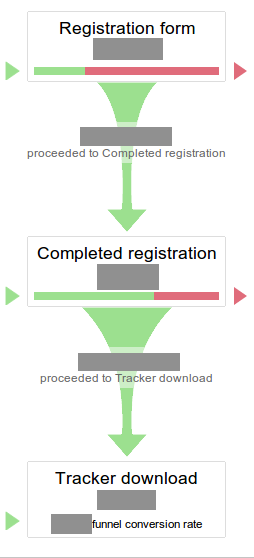
\includegraphics[width=50mm]{../images/goalfunnel}
    \end{wrapfigure}

    Bijvoorbeeld het doel van mensen aanmelden. Je kijkt dan vanaf welke pagina's mensen op het aanmeldformulier komen, en hoeveel van die mensen zich daadwerkelijk aanmelden. Het proces heet en Goal Funnel. Deze naam is gekozen omdat de gegevens vaan een trechtervorm hebben. Veel mensen komen op de homepagina, een kleiner aantal klikt door naar het formulier en een nog kleiner aantal schrijft zich daadwerkelijk in. Doel van het maken van zo'n goal funnel is om knelpunten te vinden. Zo kan er op \'e\'en bepaald punt in de rij van pagina's een probleem zitten waardoor de meeste mensen afhaken. Dit merk je omdat de trechter dan opeens v\'e\'e;l dunner wordt.

    Het doel van zo'n funnel analyseren is uitvinden op welke manier je de trechtervorm dikker kan krijgen, en dus meer mensen het door jouw gestelde doel kan laten bereiken. Doordat je op een goede manier kan laten zien waar de knelpunten zitten, kun je dit stap voor stap oplossen.

    \subsection{Bounce rates}
    Bounce Rates is de term voor het percentage wat op een pagina komt, en niet verder klikt naar andere pagina's. Een hoge bounce rate betekent doorgaans dat de pagina niet is wat de gebruiker er van verwachte op het moment dat hij de pagina bezocht. Wanneer je weet welke pagina's een hoge bounce rate hebben, kan je onderzoeken \emph{waarom} die pagina's een hoge bounce rate hebben. Bijvoorbeeld omdat de naam van de pagina niet overeenkomt met de inhoud, of omdat de informatie op de pagina niet volledig genoeg is. Vaak is het zo dat een pagina simpelweg geen goede vervolgstap biedt, en het voor de gebruiker niet duidelijk is wat hij of zij nu moet doen.

    De belangrijkste pagina met betrekking tot Bounce Rates is doorgaans de homepagina. Dit is de pagina die nieuwe bezoekers voor het eerst zien, en de pagina die ze moet overhalen om zich aan te melden. Wanneer hier geen duidelijke vervolgstap op staat, of de gebruiker wordt niet genoeg gemotiveerd, zorgt dit voor een hogere bounce rate.

    Bij Wakoopa is de homepagina de pagina met de hoogste bounce rate, ongeveer een op de twee bezoekers klikken niet verder. Als je vervolgens kijkt waar bezoekers dan w\'el op klikken, dan is met 8\% de link naar de homepagina de hoogste. Hieruit kunnen we opmaken dat voor een percentage niet duidelijk is dat het hier om de homepagina gaat. Dit kunnen we oplossen door op de homepagina niet de link naar de homepagina te laten zien.

    Daarintegen klikt een op de vier bezoekers door naar de signup pagina, waar vervolgens meer dan de helft zich ook daadwerkelijk inschrijft (dit komt uit de signup funnel). Dat zijn hoge cijfers. Niettemin moet het lukken dit hoger te krijgen door ervoor te zorgen dat mensen op de homepagina minder snel wegklikken. Onder andere het onderzoek van \cite{Hoekman2008} doet een voorstel van hoe dit verbeterd kan worden.

    \subsection{Custom tracking}
    Veel learning networks maken gebruik van \emph{AJAX}, een term die gebruikt wordt om aan te duiden dat delen van de pagina informatie van de server halen, maar niet de gehele pagina verversen. Het nadeel van deze techniek is dat er geen nieuwe \emph{page view} is, en dat dit dus ook niet automatisch met een statistiekprogramma wordt bijgehouden. In Google analytics heb je de mogelijkheid om via JavaScript zelf aan tracking te doen. Door een klein stukje code kan je aangeven dat iemand iets via AJAX heeft opgevraagd:
    \begin{verbatim}
    if(typeof(pageTracker) !== `undefined') {
      pageTracker._trackPageview(`/event/nameofevent');
    }
    \end{verbatim}
    Op deze manier kan je als learning network een hoop verschillende gebeurtenissen bijhouden. Bijvoorbeeld hoe vaak er op een banner wordt geklikt, of een comment wordt ingevoerd. Je krijgt hiermee inzicht in hoevaak een bepaalde functie wordt gebruikt.

    Op Wakoopa werd nog geen van de JavaScript opties getracked. Met behulp van van bovenstaande code is dit ingebouwd zodat we kunnen analyseren welke functies veel gebruikt worden. Ter verduidelijking zullen we een niet-bestaande boomstructuur gebruiken, in de vorm van \emph{/JavaScript/pagina-naam/naam-van-functie}. Door middel van de filters in Google Analytics kunnen deze dan gemakkelijk gevonden worden. In bijlage \ref{customtrackingappendix} staat een lijst van de functies die nu getracked worden.

    \subsection{Heatmaps}
      \begin{figure}
      \begin{center}
      \caption{Heatmap van de homepagina}
        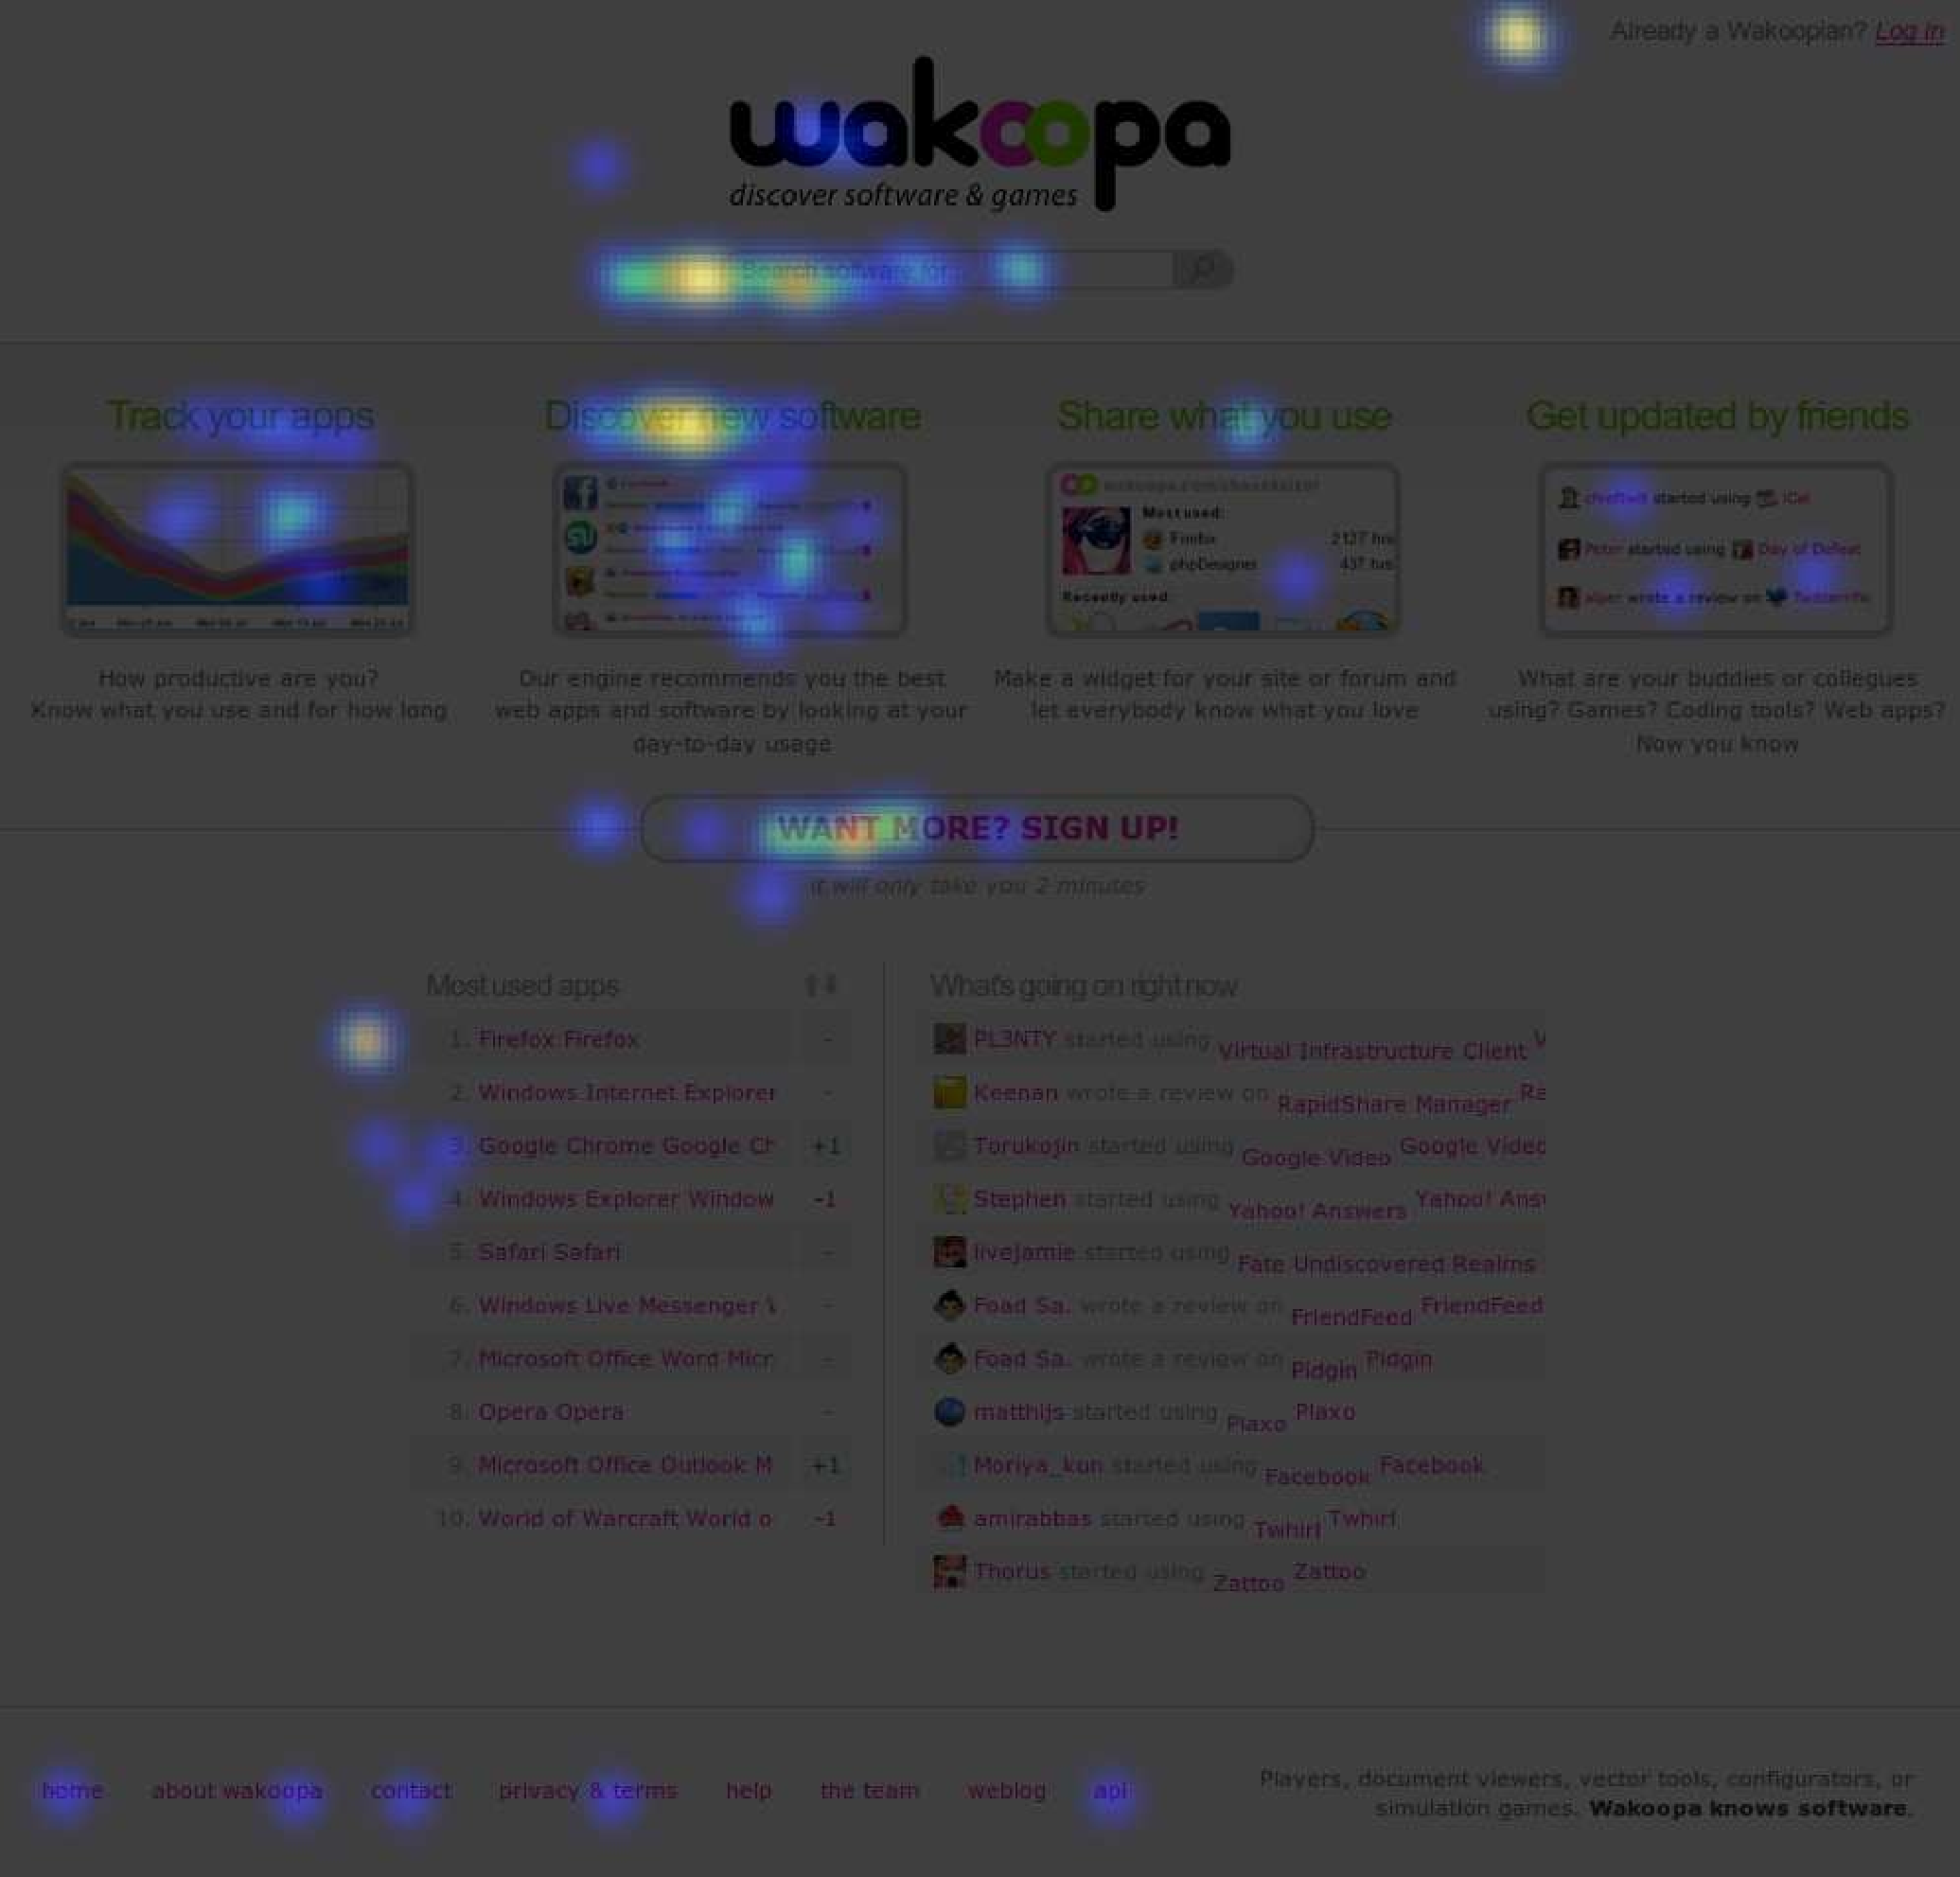
\includegraphics[width=70mm]{../images/heatmap}
      \label{heatmap}
      \end{center}
    \end{figure}
    Een techniek die pas sinds een paar jaar toegepast wordt is het maken van heatmaps. Deze heatmaps zien eruit als hittemappen, maar geven in plaats van temperatuur de hoeveelheid clicks of de positie van de muis aan op een website. Gedurende een vastgestelde periode houd je iedere click bij via JavaScript. Dit kan je dan later `plotten' op een screenshot, en zo zien waar het meest geklikt wordt. Omdat dit vrij intensief is voor de browser van de bezoeker, wordt het pas sinds recent toegepast, en nooit voor een lange duur.

    Door middel van deze techniek kan je goed zien welke delen van de pagina wel en welke delen niet worden gebruikt door je bezoekers. In Figuur \ref{heatmap} zie je een voorbeeld van de homepagina van Wakoopa, gemaakt met Crazyegg.\footnote{\url{http://crazyegg.com}} Wat hier opvalt is dat van de 4 afbeeldingen in het midden van de pagina, enkel de linker twee het meest worden aangeklikt. Hieruit kan je opmaken dat deze twee voor veel mensen interessanter zijn dan de rechter twee. Omgekeerd, de rechter twee zijn niet duidelijk genoeg, of wekken vergeleken met de linker twee niet even veel interesse. Een verbeterpunt. Het is dan aan de ontwikkelaar om te beslissen of dit betekent dat de rechter twee verbeterd moeten worden, weggehaald, of minder nadruk moeten krijgen waarbij de linker twee meer nadruk krijgen.

    Het is belangrijk om voordat je een heatmap laat genereren, te bepalen wat de doelen op een pagina zijn, waar de bezoeker moet klikken en welke delen welke soort bezoeker moeten aanspreken. Wanneer je dit doet is het achteraf gemakkelijk om te kijken in hoeverre bezoekers de pagina gebruiken op de manier dat jij bedoelde, en of de doelen die je hebt opgestelt ook daadwerkelijk behaald worden.


    \section{A/B testing}
    \textit{A/B testing, of multivariate testing, is een methode om twee (A/B) of meerdere (multivariate) variaties op een pagina of lay-out te testen, door deze gedurende een periode willekeurig onder bezoekers te verdelen. Bezoeker \emph{A} krijgt bijvoorbeeld variatie 1 te zien, en bezoeker \emph{B} krijgt variatie 2 te zien. Vervolgens kijk je welke gebruiker sneller of vaker op de door jouw gekozen link klikt of actie uitvoerd. Wanneer je dit met een groot aantal bezoekers gedurende een langere tijd doet, kan je hier statistische analyse op uitvoeren.}

    Voor A/B en multivariate testing zijn verschillende opties. De meest bekende is de Google website optimizer\footnote{\url{http://www.google.com/websiteoptimizer}}. Deze zorgt echter voor beperkingen als er dynamische content moet worden getest, omdat de vervangende HTML van te voren moet worden opgegeven. Er zijn daarom een aantal server side oplossingen. Voor Ruby on Rails zijn dit onder andere seven\_minute\_abs\footnote{\url{http://github.com/paulmars/seven\_minute\_abs}} en A/Bingo\footnote{\url{http://www.bingocardcreator.com/abingo/}}

   Wakoopa gebruikt seven\_minute\_abs vanwege de gemakkelijke implementatie. Deze automatiseert het verdelen van de verschillende opties tussen bezoekers en houd per variatie bij hoe vaak deze aangeklikt wordt.

    Naar aanleiding van de in hoofdstuk \ref{researchchapter} genoemde onderzoeken hebben we een aantal A/B tests uitgevoerd, die hieronder beschreven staan:

    \subsection{Plaats van de sign-up link op landing pages}
      \label{ctatest}
      In tegenstelling tot de homepagina hebben onze landing pages (Pagina's waar bezoekers via zoekmachines op terecht komen) wel een sign-up link in de header. Momenteel staat deze in de linkerbovenhoek. In deze A/B test bekijken we of een variate waarin deze in de rechterbovenhoek staat, tot meer clicks leidt dan wanneer deze in de linkerbovenhoek staat. De resultaten staan in Tabel \ref{tab:signupcta}, de conclusie in Hoofdstuk \ref{wak:Editorial2008}.

      \begin{table}[ht]
      \centering
      \begin{tabular}{r|*{3}{c}}
        \textbf{Versie}  & Conversie  & Verbetering & Clicks / Pageviews \\ \hline
        \textbf{Links}   & 0.00036\%  & \emph{n.v.t.}        & 1544 / 4200125 \\
        Rechts  & 0.00025\%  & -32\%                & 1058 / 4199310 \\
      \end{tabular}
      \caption{Resultaten van de sign-up link}
      \label{tab:signupcta}
      \end{table}

      \begin{figure}
        \subfigure[Links]{
\includegraphics[width=\textwidth]{../images/abtest/left}}
        \subfigure[Rechts]{
\includegraphics[width=\textwidth]{../images/abtest/right}}
        \caption{Plaats van de sign-up link op landing pages}
      \end{figure}

    \subsection{Het benoemen van de mate waarin een profiel is ingevuld}
      \label{profileprogress}
      Wakoopa geeft gebruikers al een berichtje na het inloggen wanneer een profiel nog niet volledig is ingevuld. Uit onderzoek van \cite{Brouns2008} blijkt dat het effectiever is om hier een vervolgstap of een progressiemeter neer te zetten. In deze test bekijken we een viertal variaties: De huidige berichtgeving, een berichtgeving met welk eerstvolgende veld ze nog moeten invullen (bv. Bio), een berichtgeving met een progressiemeter, en een berichtgeving met zowel een progressiemeter als wel eerstvolgende veld ingevuld moet worden.  De resultaten staan in Tabel \ref{tab:profilecta}, de conclusie in Hoofdstuk \ref{wak:Brouns2008}

        \begin{table}[ht]
        \centering
        \rowcolors{1}{white}{lightgray}
        \begin{tabular}{r|*{3}{c}}
          \textbf{Versie}                   & Conversie  & Verbetering   & Clicks / Pageviews \\ \hline
          Origineel                         & 9\%        & \emph{n.v.t.} & 502 / 5357 \\
          Met suggestie                     & 7\%        & -22\%         & 430 / 5402\\
          \textbf{Met progressiemeter}      & 15\%       & 66\%          & 819 / 5355\\
          Met beide  & 12\%       & 33\%          & 635 / 5284\\
        \end{tabular}
        \caption{Resultaten van het benoemen van de mate waarin een profiel is ingevuld}
        \label{tab:profilecta}
        \end{table}

    \begin{figure}
      \subfigure[Origineel]{
\includegraphics[width=\textwidth]{../images/abtest/original}}
      \subfigure[Met suggestie]{
\includegraphics[width=\textwidth]{../images/abtest/suggestion}}
      \subfigure[Met progressiemeter]{
\includegraphics[width=\textwidth]{../images/abtest/progresbar}}
      \subfigure[Met suggestie en progressiemeter]{
\includegraphics[width=\textwidth]{../images/abtest/both}}
      \caption{Het benoemen van de mate waarin een profiel is ingevuld}
    \end{figure}


    \subsection{De call-to-actions op de homepagina}
      \label{ctahomepagetest}

      In bijlage \ref{analysehomeappendix} staat de uitwerking van een aantal varianten voor de call-to-action afbeeldingen op de homepagina. Origineel werden er 4 functionaliteiten van Wakoopa getoont op de homepagina, zoals te zien in figuur \ref{ctahomeimg}. Deze zijn aangepast naar drie nieuwe versies: \'e\'en die vanuit de gegevens van de survey de meest gewaardeerde opties weergeeft, een versie die dat als voordelen opschrijft, en een versie die dit op een manier weergeeft die de uniekheid van een gebruiker benadrukt.
    \begin{figure}
      \begin{center}
        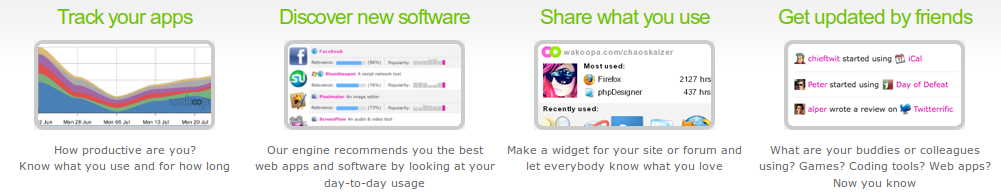
\includegraphics[width=\textwidth]{../images/newhomepage/original}
        \caption{Huidige call-to-actions op de homepagina}
        \label{ctahomeimg}
      \end{center}
    \end{figure}

        \begin{table}[ht]
        \centering
        \rowcolors{1}{white}{lightgray}
        \begin{tabular}{r|*{3}{c}}
          \textbf{Versie}                   & Conversie  & Verbetering    & Clicks / Pageviews \\ \hline
          Origineel                         & \%        & \emph{n.v.t.}   &  / \\
          Andere items                      & \%        & \%              &  / \\
          Voordelen                         & \%        & \%              &  / \\
          Uniekheid                         & \%        & \%              &  / \\
        \end{tabular}
        \caption{Resultaten van de call-to-actions op de homepagina}
        \label{tab:ctahome}
        \end{table}

  \newpage
  \chapter{Usabilitytechnieken die de participatie op een learning network verhogen}
    In dit onderzoek wordt gekeken naar de aanbevelingen voor learning networks die volgen uit de vorige hoofdstukken.

    \section{Onderzoeken}
      \subsection{\cite{Beenen2004}}
      Uit dit onderzoek komt naar voren dat het erg belangrijk is de juiste bewoordingen te kiezen. Wanneer je gebruikers teveel externe motivaties biedt, zullen ze afhaken omdat er dan het idee wordt opgewekt dat iets `moet'. Het beste werkt het wanneer de bewoording zo wordt gekozen dat gebruikers door het uitvoeren van een taak unieker worden. Hiermee benadruk je hoe een actie uitvoeren hun identiteit afzet tegen die van anderen.

      \subsection{\cite{Sohn2005}}
        Uit dit onderzoek kwamen vier punten die belangrijk zijn voor sociale netwerken:
        \begin{itemize}
          \item Maak het gemakkelijk om connecties met anderen te leggen (network density verhogen)
          \item Zorg voor stimulansen die de nieuwschierigheid van gebruikers opwekken (need for cognition)
          \item Zorg voor passieve berichtgeving van je netwerk, bijvoorbeeld wanneer connecties hun profiel wijzigen (communication directions)
          \item Zorg ervoor dat gebruikers langere tijd iets op je site te doen hebben of redenen hebben om terug te keren (web usage time)
        \end{itemize}

      \subsection{\cite{Brouns2008}}
        Dit onderzoek, wat keek welke rol identiteit speelt op een learning network, kwam met de conclusie dat het belangrijk is om mensen te stimuleren een profiel zo veel mogelijk in te vullen, en dat een progressiemeter daar goed voor werkt. Om het volledig invullen van een profiel verder te stimuleren, kan een learning network aangeven \emph{waarom} een gebruiker deze gegevens in moet vullen.

        Wat ook bleek was dat door andere gebruikers op de hoogte te brengen van wijzigingen aan iemands profiel, je ze langer ge\"interesseerd en gemotiveerd kon houden.

      \subsection{\cite{Editorial2008}}
      Uit dit onderzoek bleek dat de meest voorkomende plek van een sign up knop op een learning network rechtsboven op de homepagina was. Door dit patroon aan te houden is het voor bezoekers gemakkelijker om de knop te vinden.

      \subsection{\cite{Sloep2009}}
      Om bezoekers om te zetten in gebruikers zijn er vier voorwaarden waaraan volgens dit onderzoek moet worden voldaan. Het is belangrijk dat een gebruiker een persistente identiteit heeft, dat er geen te behalen einddoel is, dat er geen groot verschil is in de waarde van verschillende acties en dat de gebruiker zijn prestaties met anderen kan delen.

      \subsection{\cite{Wroblewski2009}}
        Inline validatie zorgt er volgens dit onderzoek voor dat gebruikers sneller een formulier doorlopen. Optimaal is het wanneer de inline validatie pas wordt weergegeven \emph{nadat} een veld is ingevuld, en dat de berichtgeving persistent is.

      \subsection{\cite{Alfrink2008}}
        Volgens \citeauthor{Alfrink2008} is het goed om de gebruiker te begeleiden en zelfs aan te geven wat de volgende stap voor deze gebruikers zou kunnen zijn. Dit wordt tegengesproken door \cite{Beenen2004}, die aangeven dat zulke externe motivatie averechts werkt. De opmerking om aan te geven waarom een bepaalde functionaliteit nut heeft komt overeen met onderzoek van \cite{Brouns2008}.

      \subsection{\cite{Hoekman2008}}
        \citeauthor{Hoekman2008} adviseren om op een homepagina de voordelen van de site te benoemen. Dit wordt tegengesproken door onderzoek van \cite{Beenen2004} en de gemaakte A/B test in sectie \ref{ctahomepagetest} en in bijlage \ref{analysehomeappendix}. \citeauthor{Hoekman2008} noemen ook kleurcodering als een sterk punt. Door bepaalde secties op een pagina een bepaalde kleur te geven, kan je deze visueel aan elkaar linken. Hiermee kan je bijvoorbeeld \emph{geel} gebruiken om alle persoonlijke informatie op een pagina aan te geven. Hierdoor wordt het voor de gebruikers gemakkelijker om te zien wat algemene informatie is, en wat specifiek op haar van toepassing is.

      \subsection{\cite{Timmerman2008}}
        \citeauthor{Timmerman2008} richt zich in zijn review vooral op het proces. Zorg dat je persona's hebt om je doelgroepen voor ogen te houden, zorg dat je door middel van A/B testen kwantitatief kan bepalen wat het beste werkt, en analyseer statistieken en clickmaps om knelpunten te vinden en op te lossen. \citeauthor{Timmerman2008} zegt dat de teksten behoeftegericht moeten worden opgestelt. Dit komt overeen met \cite{Beenen2004}, die dit `de nadruk op uniekheid leggen' noemt.

  \section{Gebruikersonderzoeken}
    \subsection{Enqu\^ete}
      Uit de enqu\^ete bleek dat een groot deel van de gebruikers na een externe impuls (het ontvangen van de nieuwsbrief) besloot de site weer te bezoeken. Dergelijke notificaties kunnen helpen met het gemotiveerd en ge\"interesseerd houden van je bezoekers.

    \subsection{Lab testen}

  \section{Technische analyse}
    \subsection{Statistieken}
      \subsubsection{Goal funnel}
        Een goal funnel voor de aanmeldprocedure kan goed inzicht geven in waar de meeste aanmeldingen vandaan komen. Je kan problemen in het aanmeldproces duidelijk zien, wanneer er bij \'e\'en bepaalde stap een scherpe daling in het voltooingspercentage is.

        Voor andere onderdelen van een site, zoals het op een later moment aanmelden voor eventuele betaalde accounts, of het koppelen van andere netwerken, kan een goal funnel worden aangemaakt om inzicht te krijgen in hoe gebruikers door het gehele proces lopen.

      \subsubsection{Bounce rates}
        Een lijst van pagina's met een hoge bounce rate bijhouden is aan te raden. Er kan dan per pagina onderzocht worden wat er mis is, of dat belangrijk is en hoe de bounce rate omlaag gebracht kan worden. Soms is een pagina niet belangrijk genoeg, bijvoorbeeld omdat er heel weinig bezoekers op komen. Afhankelijk van het aantal bezoekers en de bounce rate kan dan bepaald worden welke pagina's verbeterd moeten worden.

      \subsubsection{Custom tracking}
        Delen van de site die met JavaScript werken worden niet automatisch opgenomen in de statistieken van bijvoorbeeld Google Analytics. Om toch bij te houden hoe vaak deze functionliteit gebruikt wordt, is het slim om hier custom tracking aan toe te voegen.

      \subsubsection{Heatmaps}
        Heatmaps zijn handig om de homepagina of de signup pagina te analyseren. Er kan uitgevonden worden of de meest belangrijke elementen wel het meest bekeken worden, en welke delen er als belangrijk en minder belangrijk worden gezien. Dit soort onderzoeken zijn handig om na het invoeren van een nieuw ontwerp in te zetten.

    \subsection{A/B testen}
      Uit de in dit project uitgevoerde onderzoeken blijkt dat de uitkomst van een A/B test vaak niet is wat een ontwerper verwacht of een usability expert voorspelt. Door A/B testen direct in je learning network te implementeren kunnen aanpassingen direct getest worden.

      Omdat A/B testen op conversie toegespitst is, is het een goede methode om uit te vinden welke ontwerpen voor de meeste acties, en dus participatie, zorgen.

  \newpage
  \chapter{Welke verbeteringen zijn er specifiek voor Wakoopa door te voeren?}
    \newpage

    Dit hoofdstuk gaat expliciet in op verbeteringen voor Wakoopa, zoals gebleken uit de vorige hoofdstukken. We passen de theorie uit hoofdstuk \ref{researchchapter}, de gebruikersonderzoeken van hoofdstuk \ref{userchapter} en de data van hoofdstuk \ref{datachapter} toe op Wakoopa en beschrijven de bevindingen en aanbevelingen.

    \section{Onderzoeken}
    Naar aanleiding van de onderzoeken in hoofdstuk \ref{researchchapter} zijn er voor Wakoopa de volgende verbeteringen:

 \subsection{\cite{Beenen2004}}
      In dit onderzoek wordt veel nadruk gelegd op de \emph{call to actions}. Deze moeten een interne motivatie stimuleren, maar er niet voor zorgen dat het lijkt alsof dit een externe motivatie is. De call to actions op de homepagina zijn een goed voorbeeld om te onderzoeken of deze inderdaad voldoen aan dit vereiste.

      \paragraph{\textbf{Verbeterpunten:}}
      \begin{itemize}
        \item Call to actions op homepagina aanpassen
      \end{itemize}

    \subsection{\cite{Berlanga2007}}
    Een aantal van de punten uit het onderzoek van \citeauthor{Berlanga2007} werden in het geval van Wakoopa al gebruikt. Het is gemakkelijk om nieuwe connecties te leggen (dit kan via een enkele klik op iemands profiel) en dit wordt gestimuleerd door aan te geven welke gebruikers op jou lijken. Gebruikers krijgen een bericht wanneer hun vrienden nieuwe applicaties gebruiken, een review schrijven, een level omhoog gaan of iets op een teampagina schrijven. De effectiviteit van dit punt wordt ook ondersteund door onderzoek van \cite{Berlanga2007}. Nieuwsgierigheid wordt gestimuleerd door het puntensysteem, waarbij gebruikers meer punten verdienen door meer software te gebruiken en door acties op de site uit te voeren. Er wordt hier enkel het level getoond, en niet het totaal aantal punten. Door dit toe voegen bied je ook voor mensen die op eht hoogste level zitten een manier om zich met anderen te vergelijken. Een ander punt waar verbetering te behalen valt is het langer vasthouden van bezoekers. Wakoopa kan dit verbeteren door mensen meer acties op de site uit te laten voeren, en interessante(re) statistieken weer te geven op profielen.

      \paragraph{\textbf{Verbeterpunten:}}
      \begin{itemize}
        \item Totaal aantal punten op het profiel laten zien
        \item Bestaande functionaliteit uitbreiden
        \item Meer statistieken bieden
      \end{itemize}


    \subsection{\cite{Brouns2008}}
    \label{wak:Brouns2008}
    Wakoopa toonde enkel een melding dat een profiel nog niet compleet was, zonder vervolgstappen aan te geven. Door het implementeren van een progressiemeter zijn er 15\% meer mensen die doorklikken naar hun accountgegevens.

    Dit resultaat bleek uit een A/B test in hoofdstuk \ref{datachapter} (zie pagina \pageref{profileprogress}). Uit deze A/B test bleek dat enkel het tonen van een progressiemeter effectiever is dan het tonen van enkel een bericht, een bericht met een suggestie van een leeg veld of het tonen van een bericht met zowel een progressiemeter en een suggestie. Mogelijke verklaringen hiervoor zijn dat de zin te lang wordt wanneer er ook een suggestie in staat, of dat de suggestie velden aangeeft die mensen niet in willen vullen.

      \paragraph{\textbf{Verbeterpunten:}}
      \begin{itemize}
        \item Toevoegen van een progressiemeter met in hoeverre het profiel is gevuld
      \end{itemize}

    \subsection{\cite{Editorial2008}}
    \label{wak:Editorial2008}
    Het merendeel van de onderzochte sociale netwerken heeft een signup call to action in de rechterbovenhoek staan. Bij Wakoopa staat deze onder het logo aan de linkerkant. Door middel van een A/B test (zie pagina \pageref{ctatest}) is gekeken of dit ook voor Wakoopa meer clicks opleverde. Opvallend genoeg bleek rechts ongeveer twee keer zo slecht te werken als links. Hier zijn twee mogelijke verklaringen voor. De eerste is dat de call to action links al direct onder het logo stond, een plek waar veel mensen bij het openen van een nieuwe site als eerste kijken\footnote{\url{http://www.useit.com/alertbox/reading\_pattern.html}}. Een andere verklaring is \emph{banner blindness}. Omdat de call to action rechts naast de banner stond en het leek alsof de call to action daarbij hoorde, zullen mensen eerst de banner zien en dan automatisch de banner negeren, en daarmee ook de call to action negeren.\footnote{\url{http://www.useit.com/alertbox/fancy-formatting.html}}

      \paragraph{\textbf{Verbeterpunten:}}
      \begin{itemize}
        \item Geen
      \end{itemize}

    \subsection{\cite{Wroblewski2009}}
    Wakoopa past bij het aanmelden van een nieuwe account al de meest effectieve vorm van inline validatie toe, maar op andere plekken wordt dit nog niet gedaan. Op de account pagina kan inline validatie goed worden toegepast, om aan te geven of een nieuw wachtwoord goed genoeg is, of een wachtwoord en het controlewachtwoord overeenkomen en om aan te geven en of het ingevoerde emailadres voldoet.

      \paragraph{\textbf{Verbeterpunten:}}
      \begin{itemize}
        \item Validatie toevoegen aan de account settings pagina
      \end{itemize}

    \subsection{\cite{Alfrink2008}}
    Sinds dit rapport heeft Wakoopa een speciale pagina aangemaakt die de gebruiker direct ziet na het aanmelden, waar in stappen wordt uitgelegd welke vervolgstappen een nieuwe gebruiker heeft (de tracker downloaden, contacten zoeken, naar zijn dashboard gaan). Op andere punten kan Wakoopa dit beter stimuleren, bijvoorbeeld door middel van e-mails wanneer een gebruiker een week of twee weken lang de service niet heeft gebruikt, of alerts wanneer een gebruiker een applicatie veel gebruikt maar nog niet heeft gereviewt. Deze twee directe vragen om participatie zouden volgens \citeauthor{Alfrink2008} zeer geschikt zijn om in te zetten.

    Naast deze oproepen tot participatie noemt \citeauthor{Alfrink2008} het weergeven van persoonlijke informatie op algemene pagina's als een punt van verbetering. Sinds dit rapport wordt er al veel persoonlijke informatie weergegeven op bijvoorbeeld de software en developer-pagina's, maar niet op bijvoorbeeld de categoriepagina's. Op deze pagina kan heel goed een top-5 van door jouw gebruikte applicaties in die categorie worden laten zien.
    \paragraph{\textbf{Verbeterpunten:}}
      \begin{itemize}
        \item Alerts geven wanneer een gebruiker een applicatie langer dan vijf uur gebruikt heeft maar nog geen review heeft geschreven
        \item E-mail sturen wanneer een gebruiker twee weken geen software heeft getrackt.
        \item Een persoonlijke top 5 toevoegen op de categoriepagina's
      \end{itemize}

    \subsection{\cite{Hoekman2008}}
    Het grootste kritiekpunt uit dit onderzoek was de navigatie en de indeling van de homepagina. De homepagina had niet \'e\'en duidelijk focuspunt en de vier punten geven niet duidelijk genoeg de voordelen van Wakoopa weer. Door dit idee te A/B testen in sectie \ref{ctahomepagetest} bleek dat het benoemen van voordelen niet voor een verbetering zorgde. Voor de navigatie stellen ze voor om deze te herstructureren naar drie niveau's, gefocust op gebruikersdoelen.

    \paragraph{\textbf{Verbeterpunten:}}
      \begin{itemize}
        \item Navigatiestructuur focussen op gebruikersdoelen
      \end{itemize}


    \subsubsection{Verbetering van de navigatie}
      \citeauthor{Hoekman2008} doen een voorstel tot verbetering van de navigatie. in figuur \ref{currentnav} is de huidige navigatiestructuur van Wakoopa uitgetekend, en in figuur \ref{miskeetonav} de navigatiestructuur zoals voorgesteld in  \cite{Hoekman2008}. De sitemaps zijn gemaakt met Slickmap.\footnote{\url{http://astuteo.com/slickmap/}} Belangrijk is hierbij op te merken dat de voorgestelde navigatie niet volledig is, en als uitgangspunt bedoeld is. Zo missen de tags, updates en recommendations, die in de huidige site ook nog geen correcte plek hebben. Een ander punt wat opvalt is het gebruik van `My' om persoonlijke onderdelen aan te duiden. Wakoopa gebruikt hier `Your' voor, om het verschil tussen het learning network (wij) en de gebruiker (zij) aan te geven. Er is geen eenduidig antwoord voor welke variant beter is, en verschillende social networks gebruiken verschillende aanduidingen. Myspace en Facebook gebruiken `my', Hyves zowel `mijn' als `je', en last.fm gebruikt `your'.

      \begin{figure}
      \begin{center}
      \caption{Huidige navigatie}
        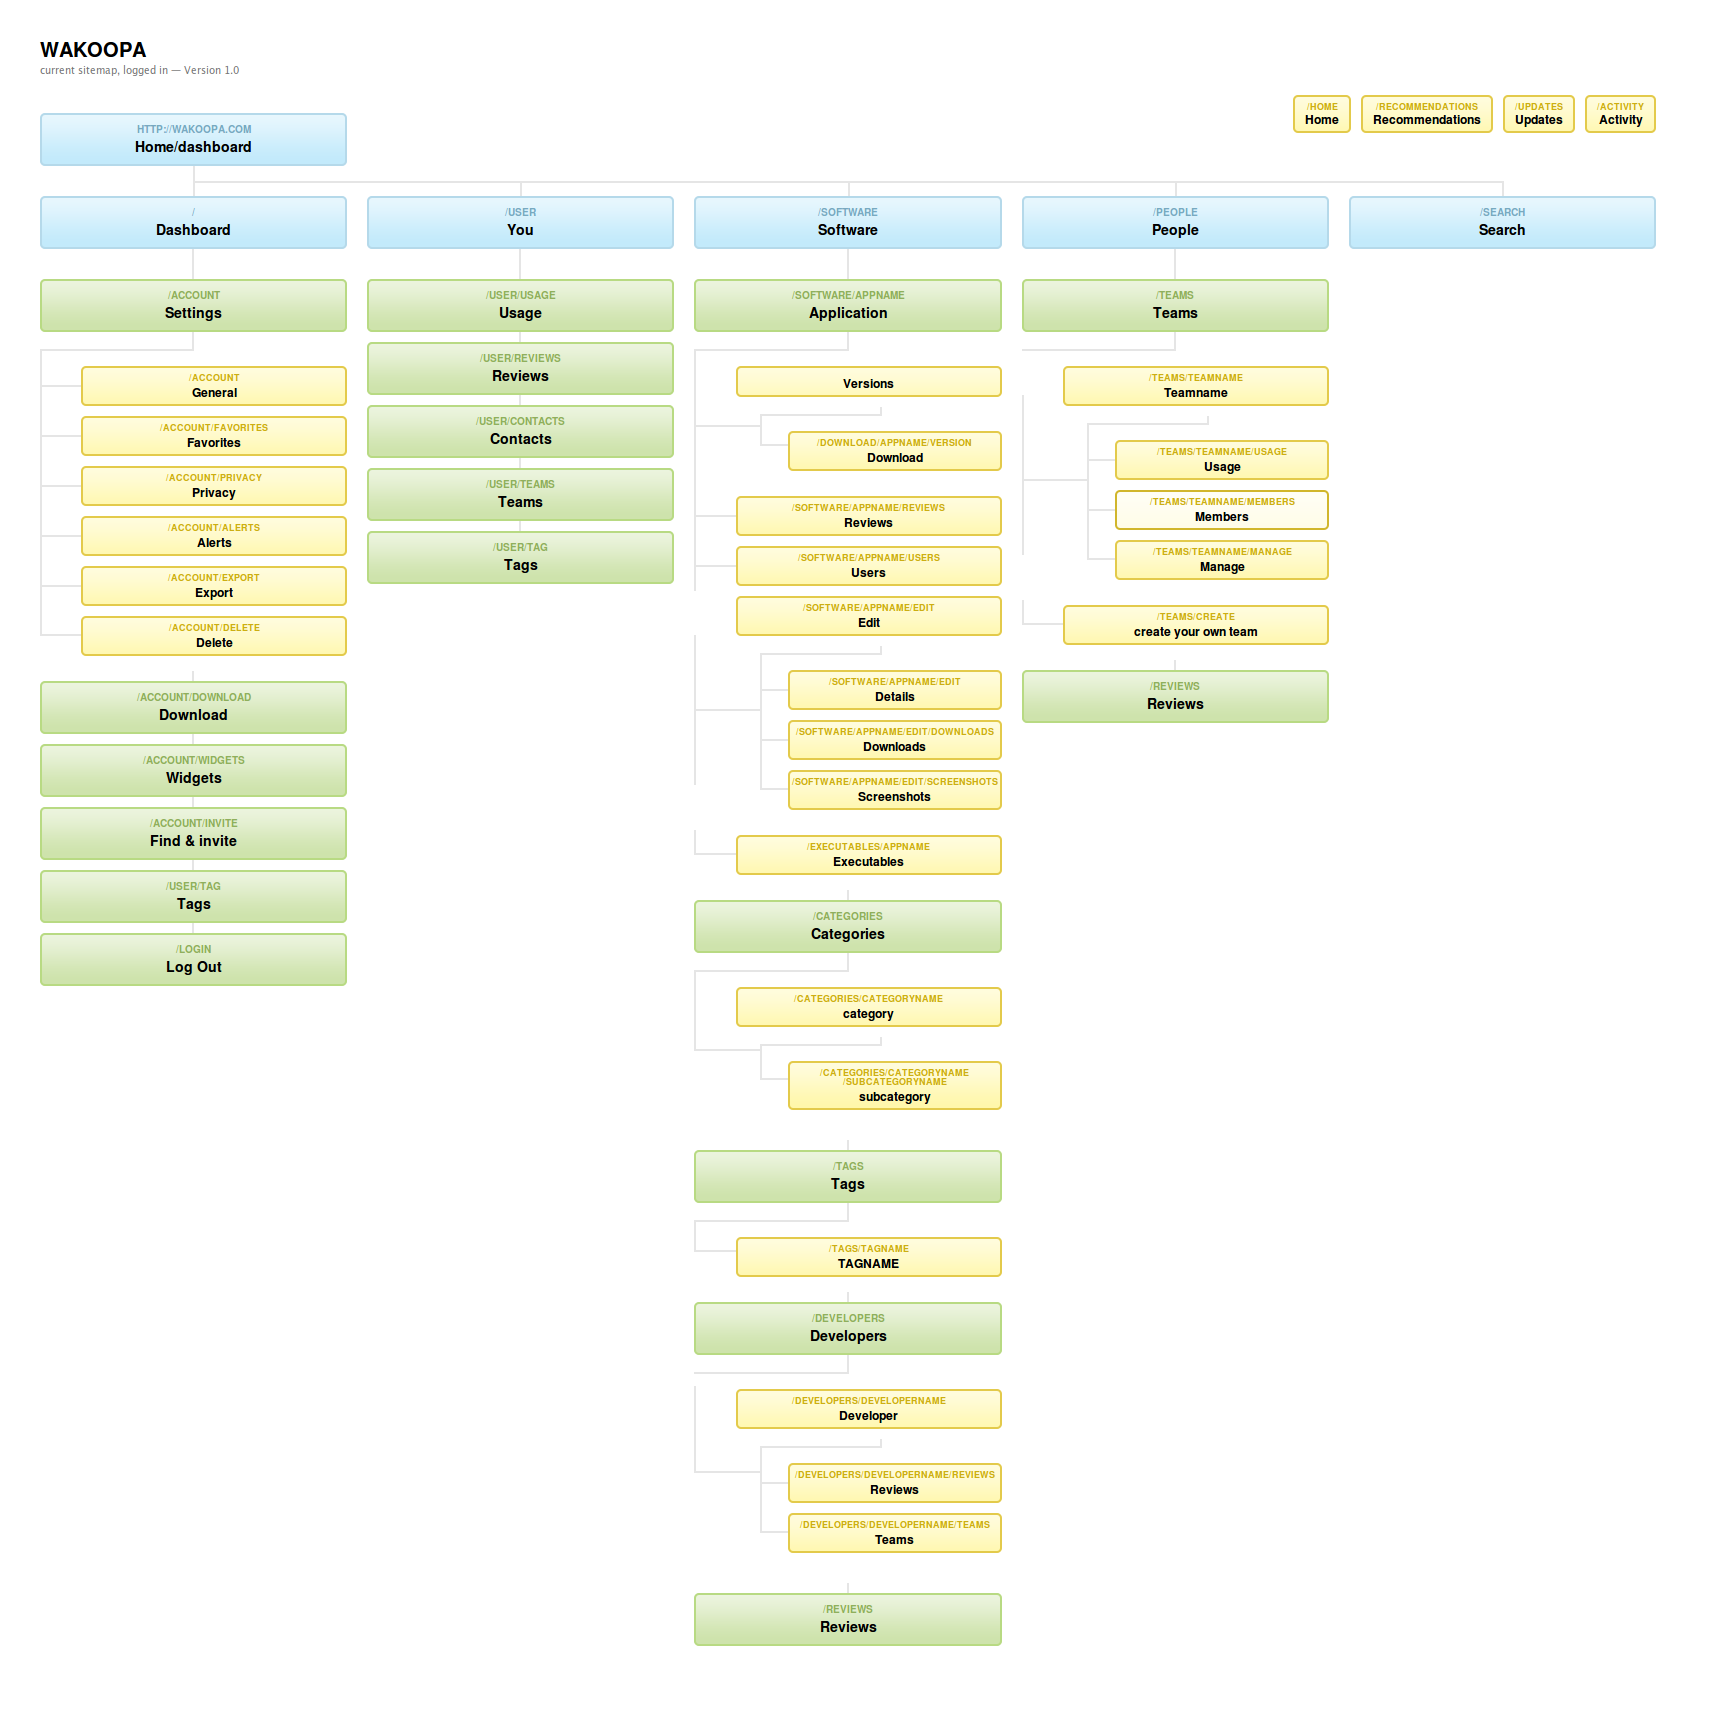
\includegraphics[width=\textwidth]{../images/currentnav}
      \label{currentnav}
      \end{center}
    \end{figure}

    \begin{figure}
      \begin{center}
      \caption{Verbeterde navigatie volgens \cite{Hoekman2008}}
        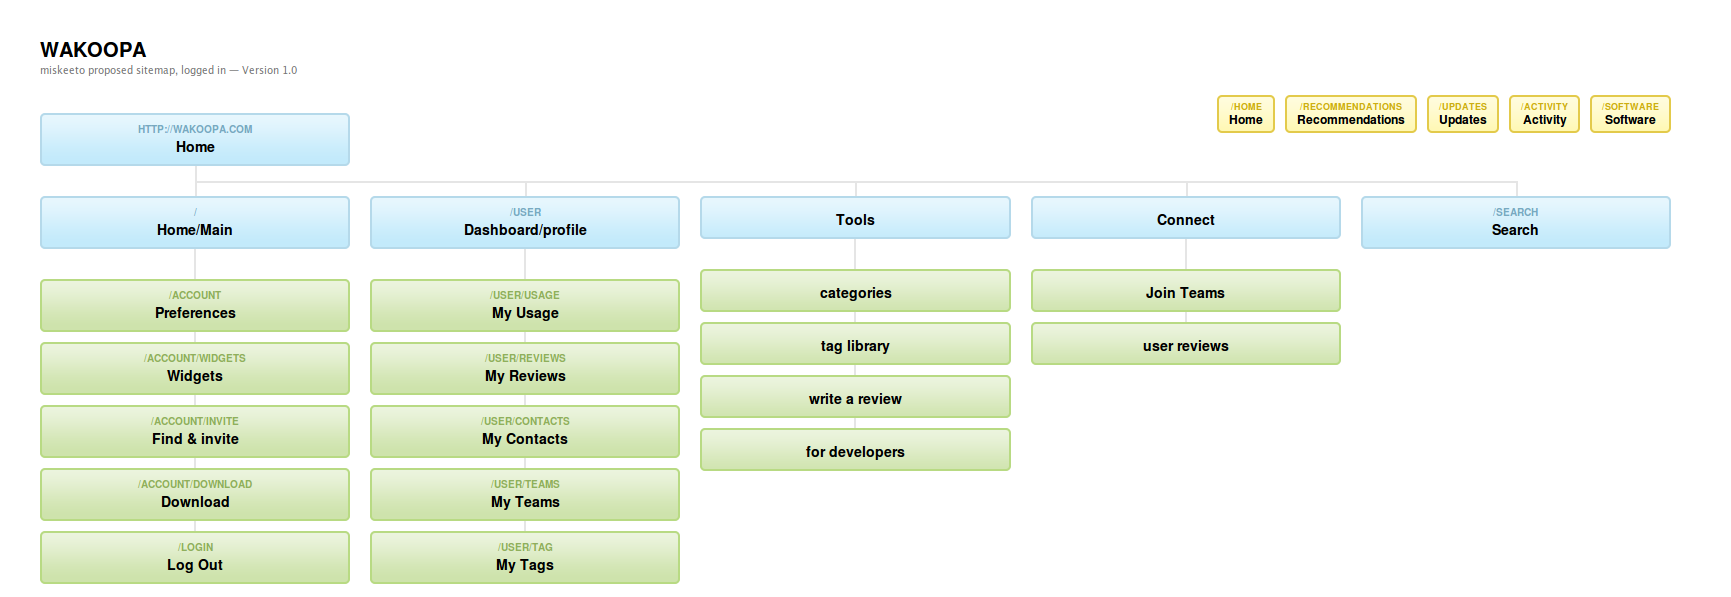
\includegraphics[width=\textwidth]{../images/miskeetonav}
      \label{miskeetonav}
      \end{center}
    \end{figure}

    \subsubsection{Navigatie workshop}
      Om te onderzoeken op welke manier de navigatie verbeterd kan worden is een navigatieworkshop met alle Wakoopa-medewerkers gehouden. Dit onderzoek is beschreven in bijlage \ref{navigationappendix}. Uit dit onderzoek kwamen een aantal kleine verbeteringen naar voren. Teams, categories en developers worden meer naar voren gepracht dan in de huidige navigatie. Het downloaden van de tracker is voor iedereen toegankelijk geworden, en als laatste wordt er een duidelijkere verdeling gemaakt tussen wat er bij een gebruiker zijn publieke profiel, en bij het persoonlijke gedeelte van een account hoort.

    \subsection{\cite{Timmerman2008}}
    In dit onderzoek wordt veel verwezen naar het analyseren van data en gebruik van andere usabilitytechnieken dan een expert review. Het analyseren van Statistieken, het gebruik van A/B testen en het maken van persona's worden als nuttige middelen genoemt. Door middel van deze persona's kan bij (nieuwe) functionaliteit worden gekeken of dit wel overeenkomt met gebruikersdoelen.

    \paragraph{\textbf{Verbeterpunten:}}
      \begin{itemize}
        \item Maak persona's en gebruikersdoelen
        \item Analyseer de statistieken op trends
      \end{itemize}

    \subsubsection{Persona's}
      In bijlage \ref{personasappendix} zijn persona's voor Wakoopa gemaakt. Deze zijn opgestelt aan de hand van \cite{Klompsma} en gebaseerd op de enqu\^ete en de doelgroepsanalyse die door Wakoopa intern is gemaakt. \cite{Klompsma} combineert het maken van persona's gebaseerd op doelgroepen met een analyse van het soort persoon. Dit doet hij aan de hand van een variatie op de Myer Briggs type indicator (Dit is een psychologische test die je in een van de zestien voorkeurscategorie\"en indeelt) zoals beschreven in \cite{Williams}. In dit boek vertaalt auteur Roy Williams de zestien categorieren naar vier soorten gebruikers, op basis van twee vragen:
      \begin{itemize}
        \item Ben je een snelle of langzame beslisser?
        \item Beslis je op basis van feiten of op basis van emotie?
      \end{itemize}

      \paragraph{}De vier gebruikers die hier uit voortkomen zijn:

      \begin{itemize}
        \item de competitieve gebruiker
          Deze mensen beslissen snel en op basis van feiten
        \item De methodische gebruiker
          Deze mensen beslissen langzaam en op basis van feiten
        \item De spontane gebruiker
          Deze mensen beslissen snel en op basis van emotie
        \item De humanistische gebruiker
          Deze mensen beslissen langzaam en op basis van emotie
      \end{itemize}

      In de persona's voor Wakoopa komen twee competitieve, een spontane en een humanistische gebruiker voor. Het is voor deze doelgroepen belangrijk dat de juiste informatie snel op een goede manier wordt gepresenteerd.

    \section{Gebruikersonderzoek}
      \subsection{Enqu\^ete}
        De meeste respondenten gaven aan de site te bezoeken in reactie op het ontvangen van de wekelijkse nieuwsbrief. Deze nieuwsbrief werd voorheen met de hand verstuurd, en werd daardoor soms niet verstuurd. Naar aanleiding van de enqu\^ete is er voor gekozen om automatisch een wekelijkse mail te versturen, zonder extra introtekst erbij.

        Veel respondenten lieten weten dat de informatie over software niet toereikend genoeg was. De reden die de meesten gaven was dat het moeilijk is interessante reacties te vinden. Hiervoor zou er een stem-systeem moeten worden ingebouwd, waarbij de reacties met de hoogste stemmen bovenaan komen staan, en waar mensen reacties op reacties kunnen plaatsen (een zogenaame threaded discussie).

        Ondanks de mogelijkheid om softwarepagina's gemakkelijk te delen via andere sociale netwerken, bleken veel mensen dit te missen. Daarom is de "share" knop vervangen met een groep icoontjes. Deze iconen zijn duidelijker herkenbaar. Dit is nog verder uit te breiden met functionaliteit die automatisch berichten op andere sociale netwerken plaatst, bijvoorbeeld als een gebruiker een review schrijft.

      \paragraph{\textbf{Verbeterpunten:}}
      \begin{itemize}
        \item Verstuur iedere week een nieuwsbrief
        \item Threaded discussies toevoegen op de softwarepagina's en stemmogelijkheden toevoegen
        \item Reacties op softwarepagina's sorteren op aantal stemmen
        \item Het toevoegen van automatisch plaatsen van berichten op andere sociale netwerken
      \end{itemize}


    \section{Statistieken}
    \subsection{Bounce Rates}

    \subsection{Custom tracking}
    Na het toevoegen van custom tracking was er meer inzicht in welke JavaScriptfunctionaliteit het meest gebruikt werd. Voornamelijk interessant was welke grafieken het meest bekeken werden. grafieken van dagelijks gebruik zijn meer dan twee keer zo populair als de overige grafieken. Een verbetering hier zou dus zijn standaard deze grafiek te laten zien. Wat ook opvalt is dat het bekijken van redenaties achter aanbevelingen, en het verwijderen van niet geschikte aanbevelingen erg vaak gebeurd. Het verwijderen van aanbevelingen gebeurd bijna evenveel als het bekijken van redenaties achter aanbevelingen.

    Het toevoegen van favorites gebeurd bijna driemaal zovaak als het toevoegen van tags. Dit is te verklaren met het feit dat favorites op de site vrij gemakkelijk te vinden zijn, terwijl dit bij tags nog niet het geval is. Een conclusie zou kunnen zijn dat mensen favorites als een `gemakkelijke' of socialere vorm van taggen zien.

    \paragraph{\textbf{Verbeterpunten:}}
      \begin{itemize}
        \item Toon de meest interessante grafiek als eerste
        \item Maak tagging duidelijker
      \end{itemize}

    \subsection{A/B testen}
      \subsubsection{Plaats van de sign-up link op landing pages}
        In sectie \ref{ctatest} blijkt uit de resultaten dat de sign-up link aan de linkerkant beter werkt dan die aan de rechterkant. Dit was de originele positie, en na afloop van de A/B test blijft de link daar staan.

    \paragraph{\textbf{Verbeterpunten:}}
      \begin{itemize}
        \item geen
      \end{itemize}

      \subsubsection{Het benoemen van de mate waarin een profiel is ingevuld}
        In sectie \ref{profileprogress} blijkt uit de resultaten hoewel zowel een progressiemeter als een suggestie beter werkten dan enkel een bericht, ze samen percentueel voor minder verbetering zorgen dank enkel de progressiemeter. Daarom is enkel de progressiemeter geimplementeerd.

    \paragraph{\textbf{Verbeterpunten:}}
      \begin{itemize}
        \item het toevoegen van een progressiemeter om aan te geven in welke mate je profiel is ingevuld.
      \end{itemize}

  \newpage
  \chapter{De quick wins om participatie te verhogen op learning networks}
    \newpage

  \newpage
  \chapter*{Conclusie en Aanbevelingen}
  \addcontentsline{toc}{chapter}{Conclusie en Aanbevelingen}

  \newpage
  \chapter*{Discussie}
  \addcontentsline{toc}{chapter}{Discussie}

  \listoftables
  \addcontentsline{toc}{chapter}{Lijst van tabellen}

  \listoffigures
  \addcontentsline{toc}{chapter}{Lijst van figuren}


  \newpage
  \bibliography{../references/referenties}
  \bibliographystyle{../references/agsm2}
  \addcontentsline{toc}{chapter}{Bibliografie}
  \newpage

  \appendix
  \addappheadtotoc
  \chapter{Analyse homepagina: call to actions}
\label{analysehomeappendix}
\textit{3 november 2009} De vier punten op de huidige homepagina van Wakoopa noemen enkel functionaliteit, in plaats van voordelen (\citet{Hoekman2008}) of uniekheid van gebruikers (\citet{Beenen2004}). Door de call-to-actions aan te passen naar een van deze twee uitgangspunten, zou het aantal aanmeldingen (en dus de participatie) moeten verhogen.

\paragraph{huidig:}
\begin{itemize}
    \item{Track your apps\\
      How productive are you?\\
      Know what you use and for how long}

    \item{Discover new software\\
      Our engine recommends you the best web apps and software by looking at your day-to-day usage}

    \item{Share what you use\\
      Make a widget for your site or forum and let everybody know what you love}

    \item{Get updated by friends\\
      What are your buddies or colleagues using? Games? Coding tools? Web apps? Now you know}
\end{itemize}

Naast de bewoording van deze punten, kunnen we ook inhoudelijk kijken naar de punten. Wanneer we de survey bekijken, blijkt dat slechts een derde van de huidige gebruikers wel eens een widget op zijn blog of facebook heeft gezet. Voor het overgrote deel van de gebruikers was dit dus niet een reden om zich aan te melden, en daarmee zijn er wellicht andere functies die bezoekers meer prikkelen. Nieuwe functionaliteit waar huidige gebruikers het meest enthousiast over zijn zijn de aanbevelingen en het web tracking. Deze twee functionaliteiten komen niet duidelijk naar voren. De aanbevelingen worden genoemd, maar slechts indirect, en hetzelfde geld voor web apps.Kijkend naar de enqu\^ete kunnen deze beter prominent in beeld worden gebracht.

Na Web tracking en aanbevelingen zijn de twee grootste nieuwe functionaliteiten waar gebruikers tevreden over zijn het tracken op linux en het reputatie en puntensysteem. Kijkend naar de huidige homepagina staat er nergens op welke platformen wakoopa ge\"installeerd kan worden, en welke worden getrackt. ook het reputatie en puntensysteem wordt niet genoemd, terwijl een significant deel van de gebruikers aangeeft dit een waardevolle toevoeging te vinden.

Met bovenstaande punten kunnen we een nieuw lijstje maken met daarin de functionaliteiten die het belangrijkst zijn en die door huidige gebruikers het meest gewaardeerd worden:
\begin{itemize}
    \item{Track what you use\\
      Keep track of what you use on Windows, Mac OS X, Linux and the web}

    \item{Get recommendations\\
      We analyse your day-to-day usage and recommend you new software}

    \item{Updates from friends\\
      See which applications your friends use and what they think of them}

    \item{Collect awards\\
      Level up to become a Wakoopa overlord and compare with friends}
\end{itemize}

Deze functionele items kunnen we vervolgens omvormen naar een lijst met persoonlijke voordelen, en een lijst met nadruk op de uniekheid van gebruikers:

\paragraph{Voordelen (\citet{Hoekman2008}) }
\begin{itemize}
    \item{Gain insight\\
      Keep track of what you use on Windows, Mac OS X, Linux and the web}

    \item{Find better applications\\
      We analyse your day-to-day usage and recommend you new software}

    \item{Match with friends\\
      See which applications your friends use, what they think of them}

    \item{Become an overlord\\
      Use Wakoopa, get awards and reach the highest level}
\end{itemize}
\paragraph{Uniekheid (\citet{Beenen2004})}
\begin{itemize}
    \item{Find your usage patterns\\
      Keep track of what you use on Windows, Mac OS X, Linux and the web}

    \item{Personal recommendations\\
      We analyse your day-to-day usage and recommend you new software}

    \item{Do you differ from friends?\\
      See which applications your friends use and what they think of them}

    \item{Compete with friends\\
      Use Wakoopa, get awards and become a Wakoopa overlord}
\end{itemize}

    \begin{figure}
      \begin{center}
      \caption{Grafische weergave}
        \subfigure[Origineel]{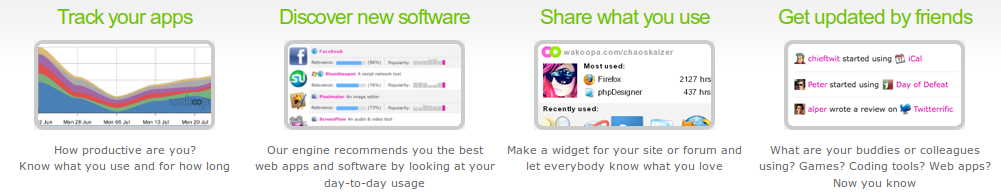
\includegraphics[width=\textwidth]{../images/newhomepage/original}}
        \subfigure[Andere items]{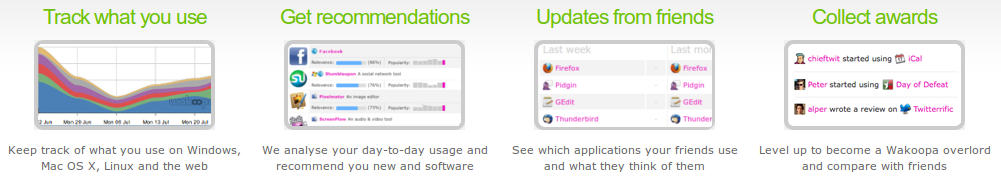
\includegraphics[width=\textwidth]{../images/newhomepage/improved}}
        \subfigure[Voordelen]{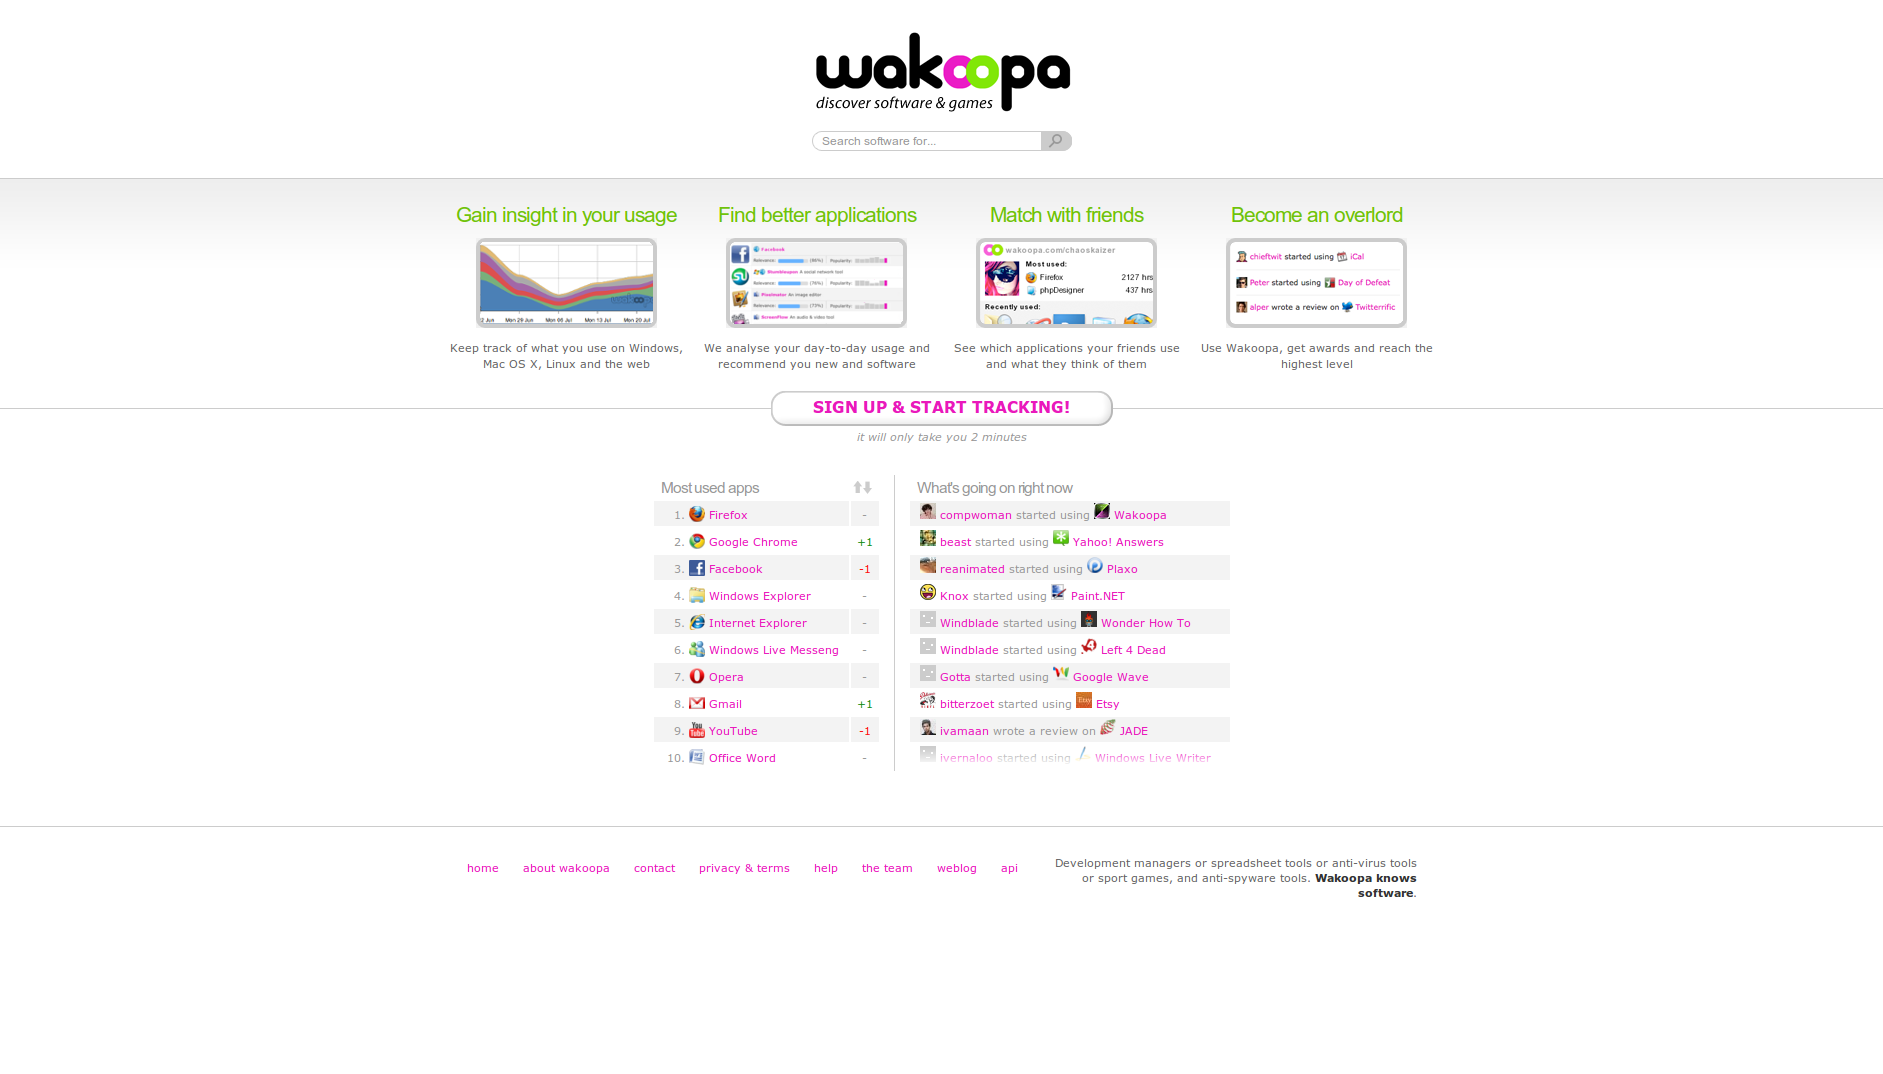
\includegraphics[width=\textwidth]{../images/newhomepage/benefits}}
        \subfigure[Uniekheid]{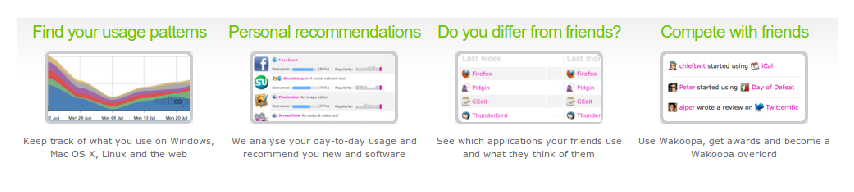
\includegraphics[width=\textwidth]{../images/newhomepage/uniqueness}}
      \end{center}
    \end{figure}


  \chapter{Navigatie brainstorm}
    \label{navigationappendix}
\textit{28 oktober 2009} Door middel van een brainstorm over de navigatie van Wakoopa is er een sitemap opgesteld. De brainstorm is uitgevoerd door het Team van Wakoopa (Wouter, Robert, Menno, Mark en Marten), wat betekent dat er voorkennis aanwezig was. Dit is deels tegengegaan doordat er twee personen bij waren die minder bekend waren met de huidige navigatie, Mark en Marten. Er is uitgegaan van een ingelogde status, een status waarbij de gebruiker toegang heeft tot zijn eigen gegevens. Statische pagina's zoals Privacy, About en FAQ zijn voor deze brainstorm buiten beschouwing gelaten, omdat ze niet actief deel hebben in gebruik van de website.

Van tevoren waren alle bestaande pagina's op post-its geschreven, en deze zijn verdeeld over de aanwezigen met de opdracht om deze gezamelijk op een A1 vel te plakken, waarbij gelijk pagina's geclusterd werden en de hi\"erarchie aangegeven werd door post-its onder elkaar te plakken. Hier werd expliciet gevraagd niet aan de huidige navigatie vast te houden, maar het zo neer te leggen dat het voor de personen zo logisch mogelijk was. Bijgevoegd waren pennen, waarmee de deelnemers toevoegingen of verduidelijkingen op of om de post-its konden schrijven.

\section*{Uitkomst}
De website werd ingedeeld in zeven hoofdsecties: Home, dashboard, application, people, teams, categories en developers.. Dit is iets anders dan de huidige site, die Home/dashboard, Software, People en Search als hoofdsecties heeft. Het downloaden van de tracker staat momenteel onder het dashboard, maar werd liever direct onder Home gezien, met de beredenatie dat iedereen in principe de tracker mag downloaden. Een ander tweedeling is die van informatie over een gebruiker. Een deel daarvan hoort onder het dashboard (jouw persoonlijke accountpagina) en het ander onder You, je publieke profiel. Uit de workshop bleek dat een aantal van deze dingen niet op de goede plek stonden en beter zouden kloppen wanneer ze onder het persoonlijke dan wel publieke deel van Wakoopa zouden staan.
\section*{Vergelijking met \citeauthor{Hoekman2008}}
Kijkend naar de verbeteringen zoals voorgesteld door \citeauthor{Hoekman2008} (zie figuur \ref{miskeetonav2}) kun je zien dat de uitkomst van de workshop tussen de huidige site en de verbeteringen van \citeauthor{Hoekman2008} in zit. Hoewel de benaming en de pagina's hetzelfde blijven als op de huidige site, met slechts hier en daar een bijgeschreven verbetering, neigt de verdeling van de pagina's meer naar de indeling van \citeauthor{Hoekman2008}. Waar de verbeterde versie van \citeauthor{Hoekman2008} een compleet nieuwe indeling is, kwam er uit de workshop een gefinetunede versie van de huidige navigatie.

      \begin{figure}
      \begin{center}
      \caption{Huidige navigatie}
        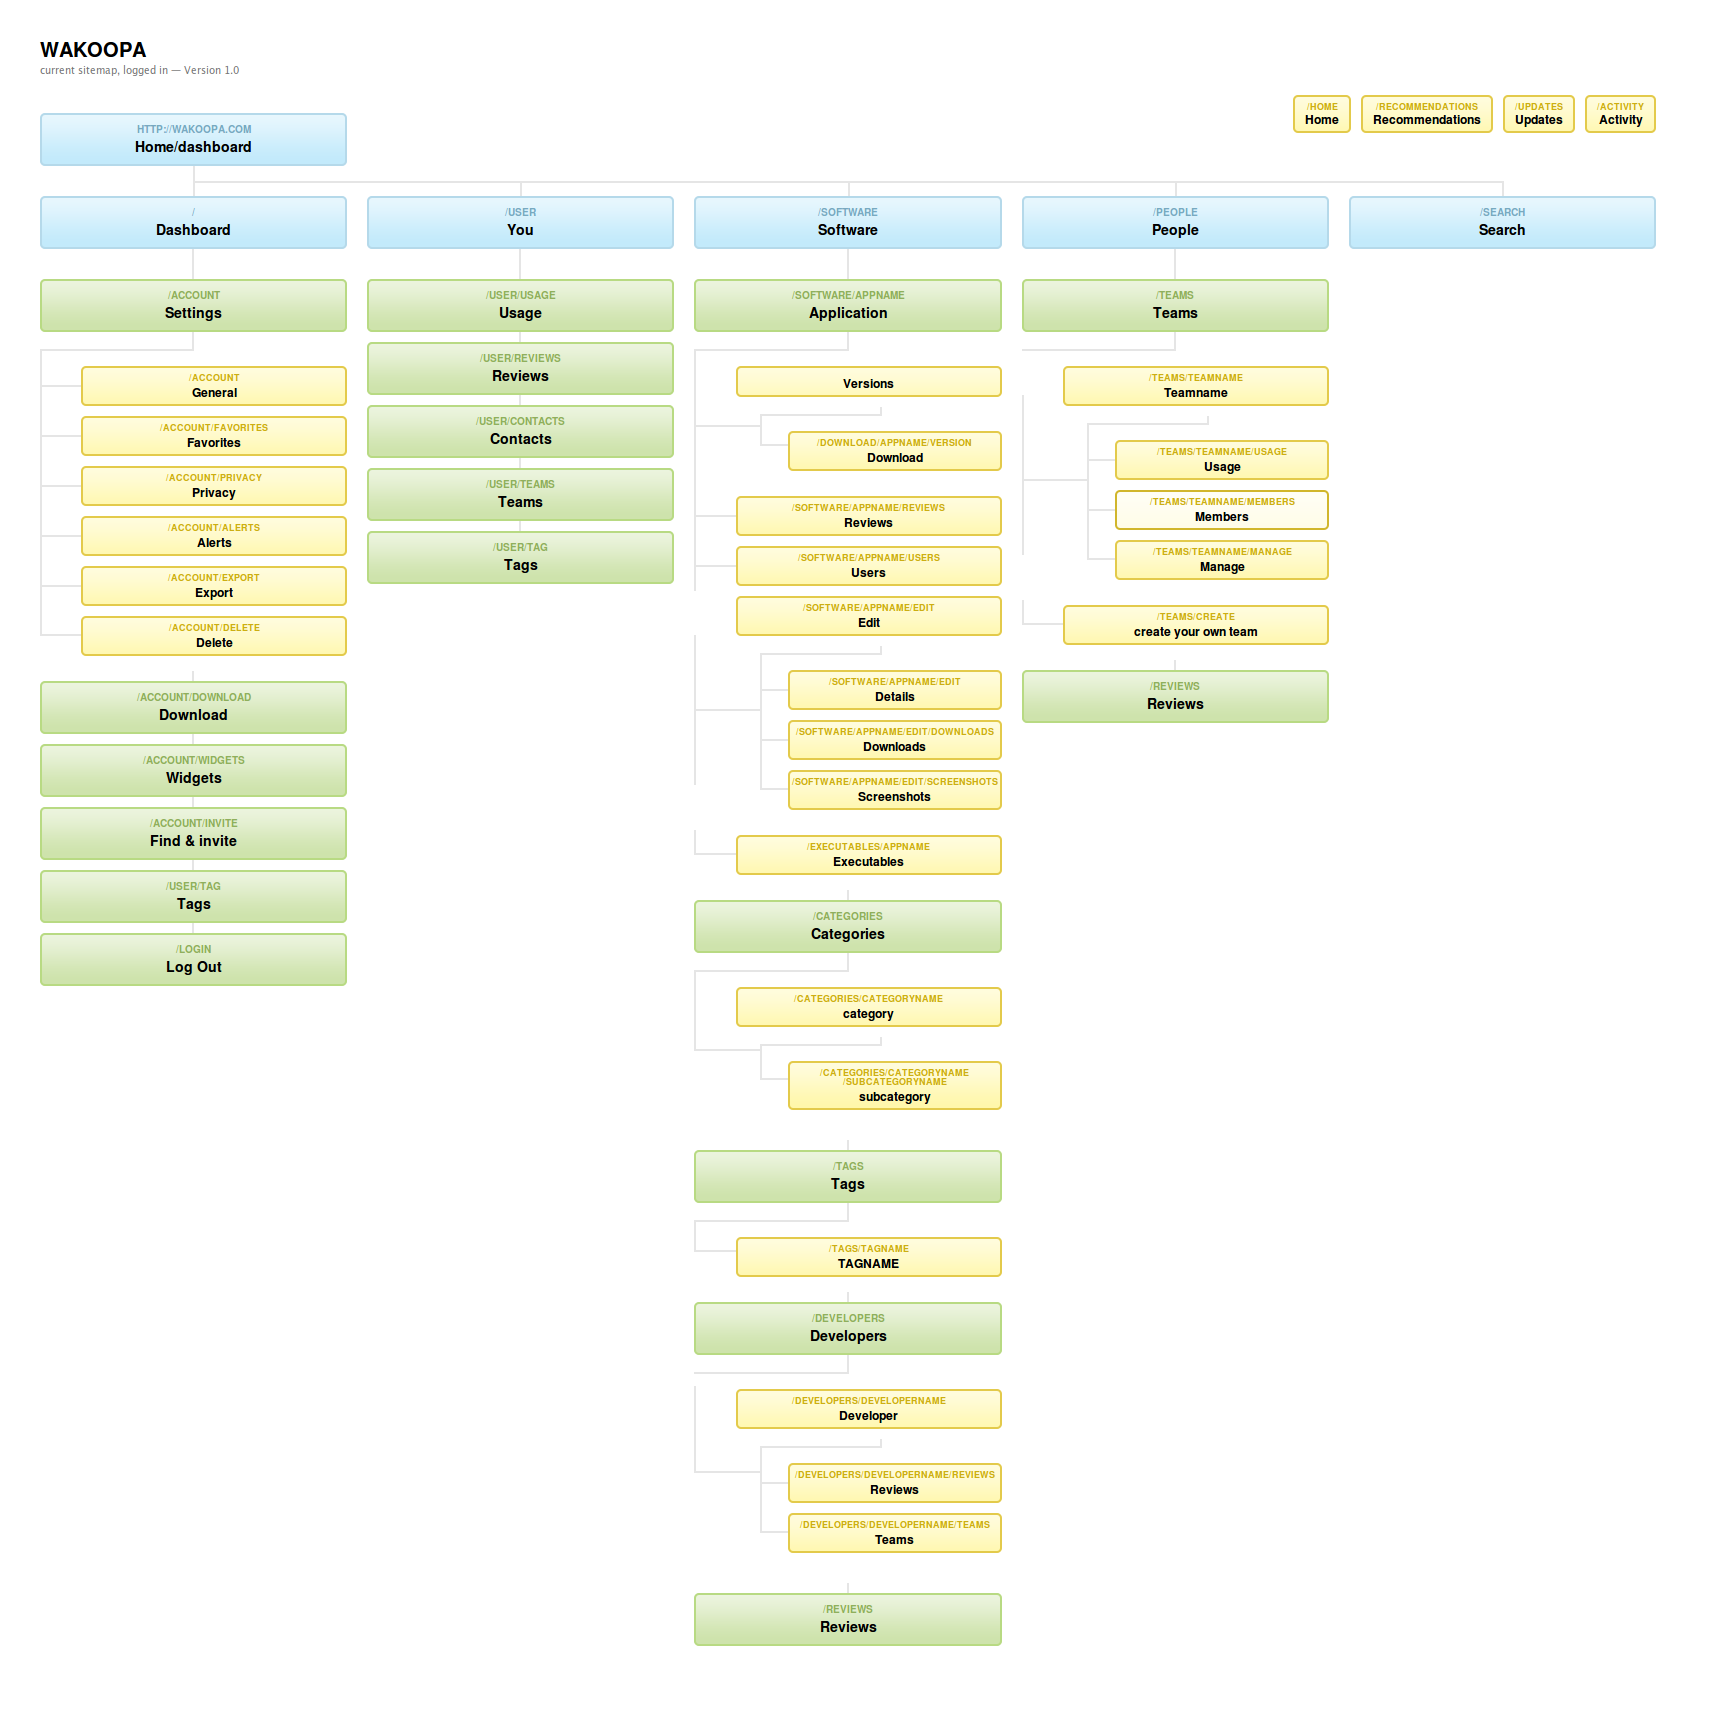
\includegraphics[width=\textwidth]{../images/currentnav}
      \end{center}
    \end{figure}

    \begin{figure}
      \begin{center}
      \caption{Verbeterde navigatie volgens \cite{Hoekman2008}}
        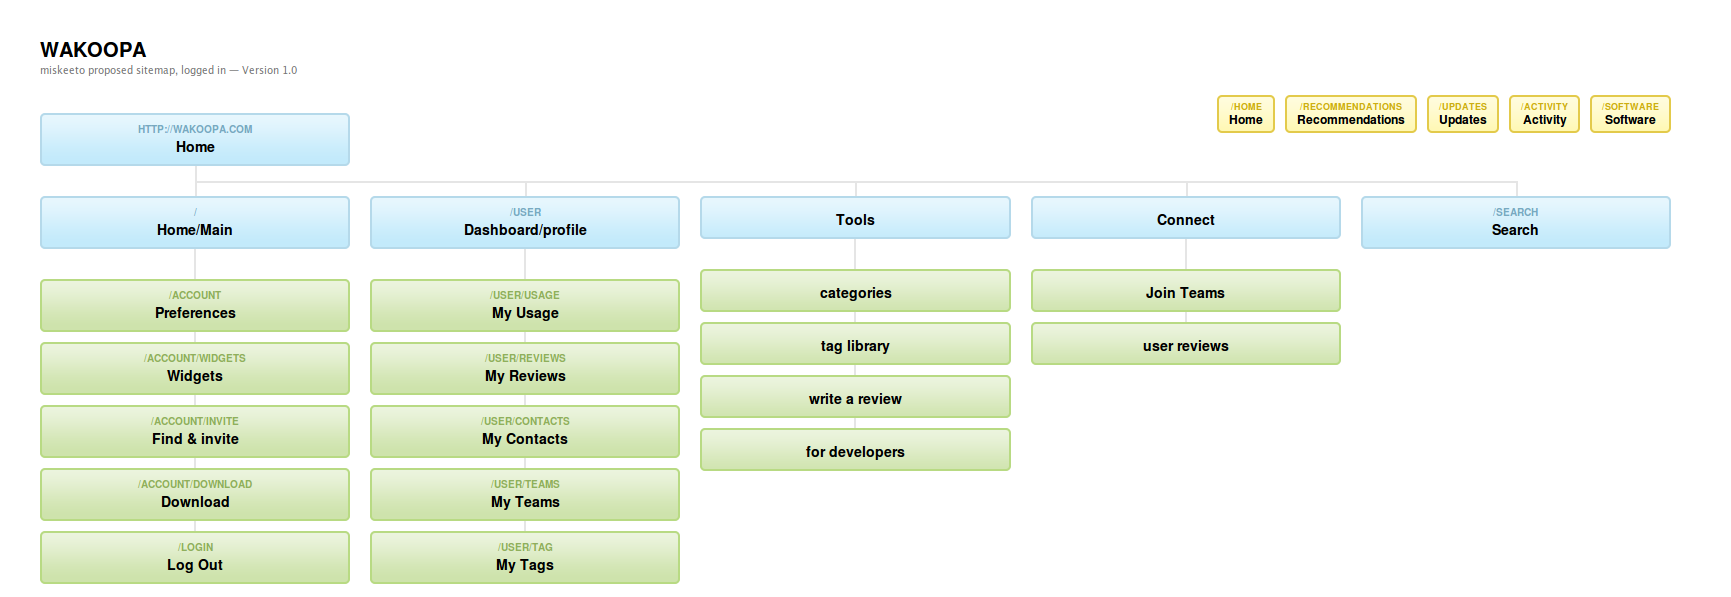
\includegraphics[width=\textwidth]{../images/miskeetonav}
      \label{miskeetonav2}
      \end{center}
    \end{figure}

      \begin{figure}
      \begin{center}
      \caption{Verbeterde navigatie volgens Navigatie workshop}
        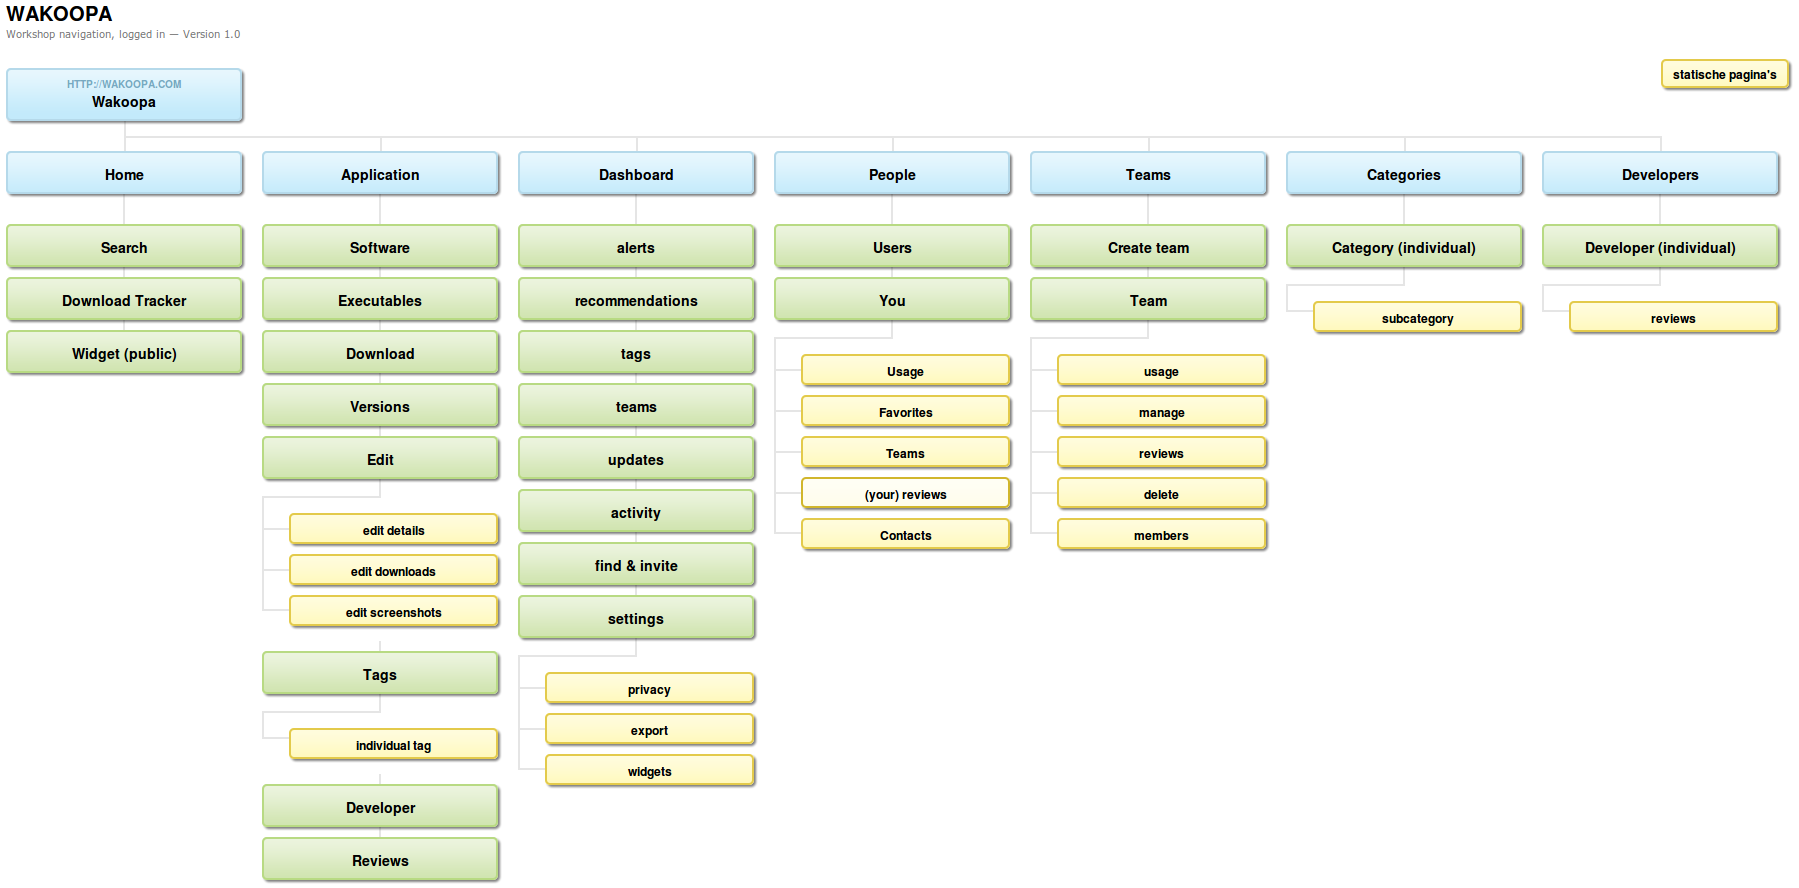
\includegraphics[width=\textwidth]{../images/workshopnav}
      \end{center}
    \end{figure}

    \begin{figure}
      \begin{center}
      \caption{Foto's van de workshop}
        \subfigure{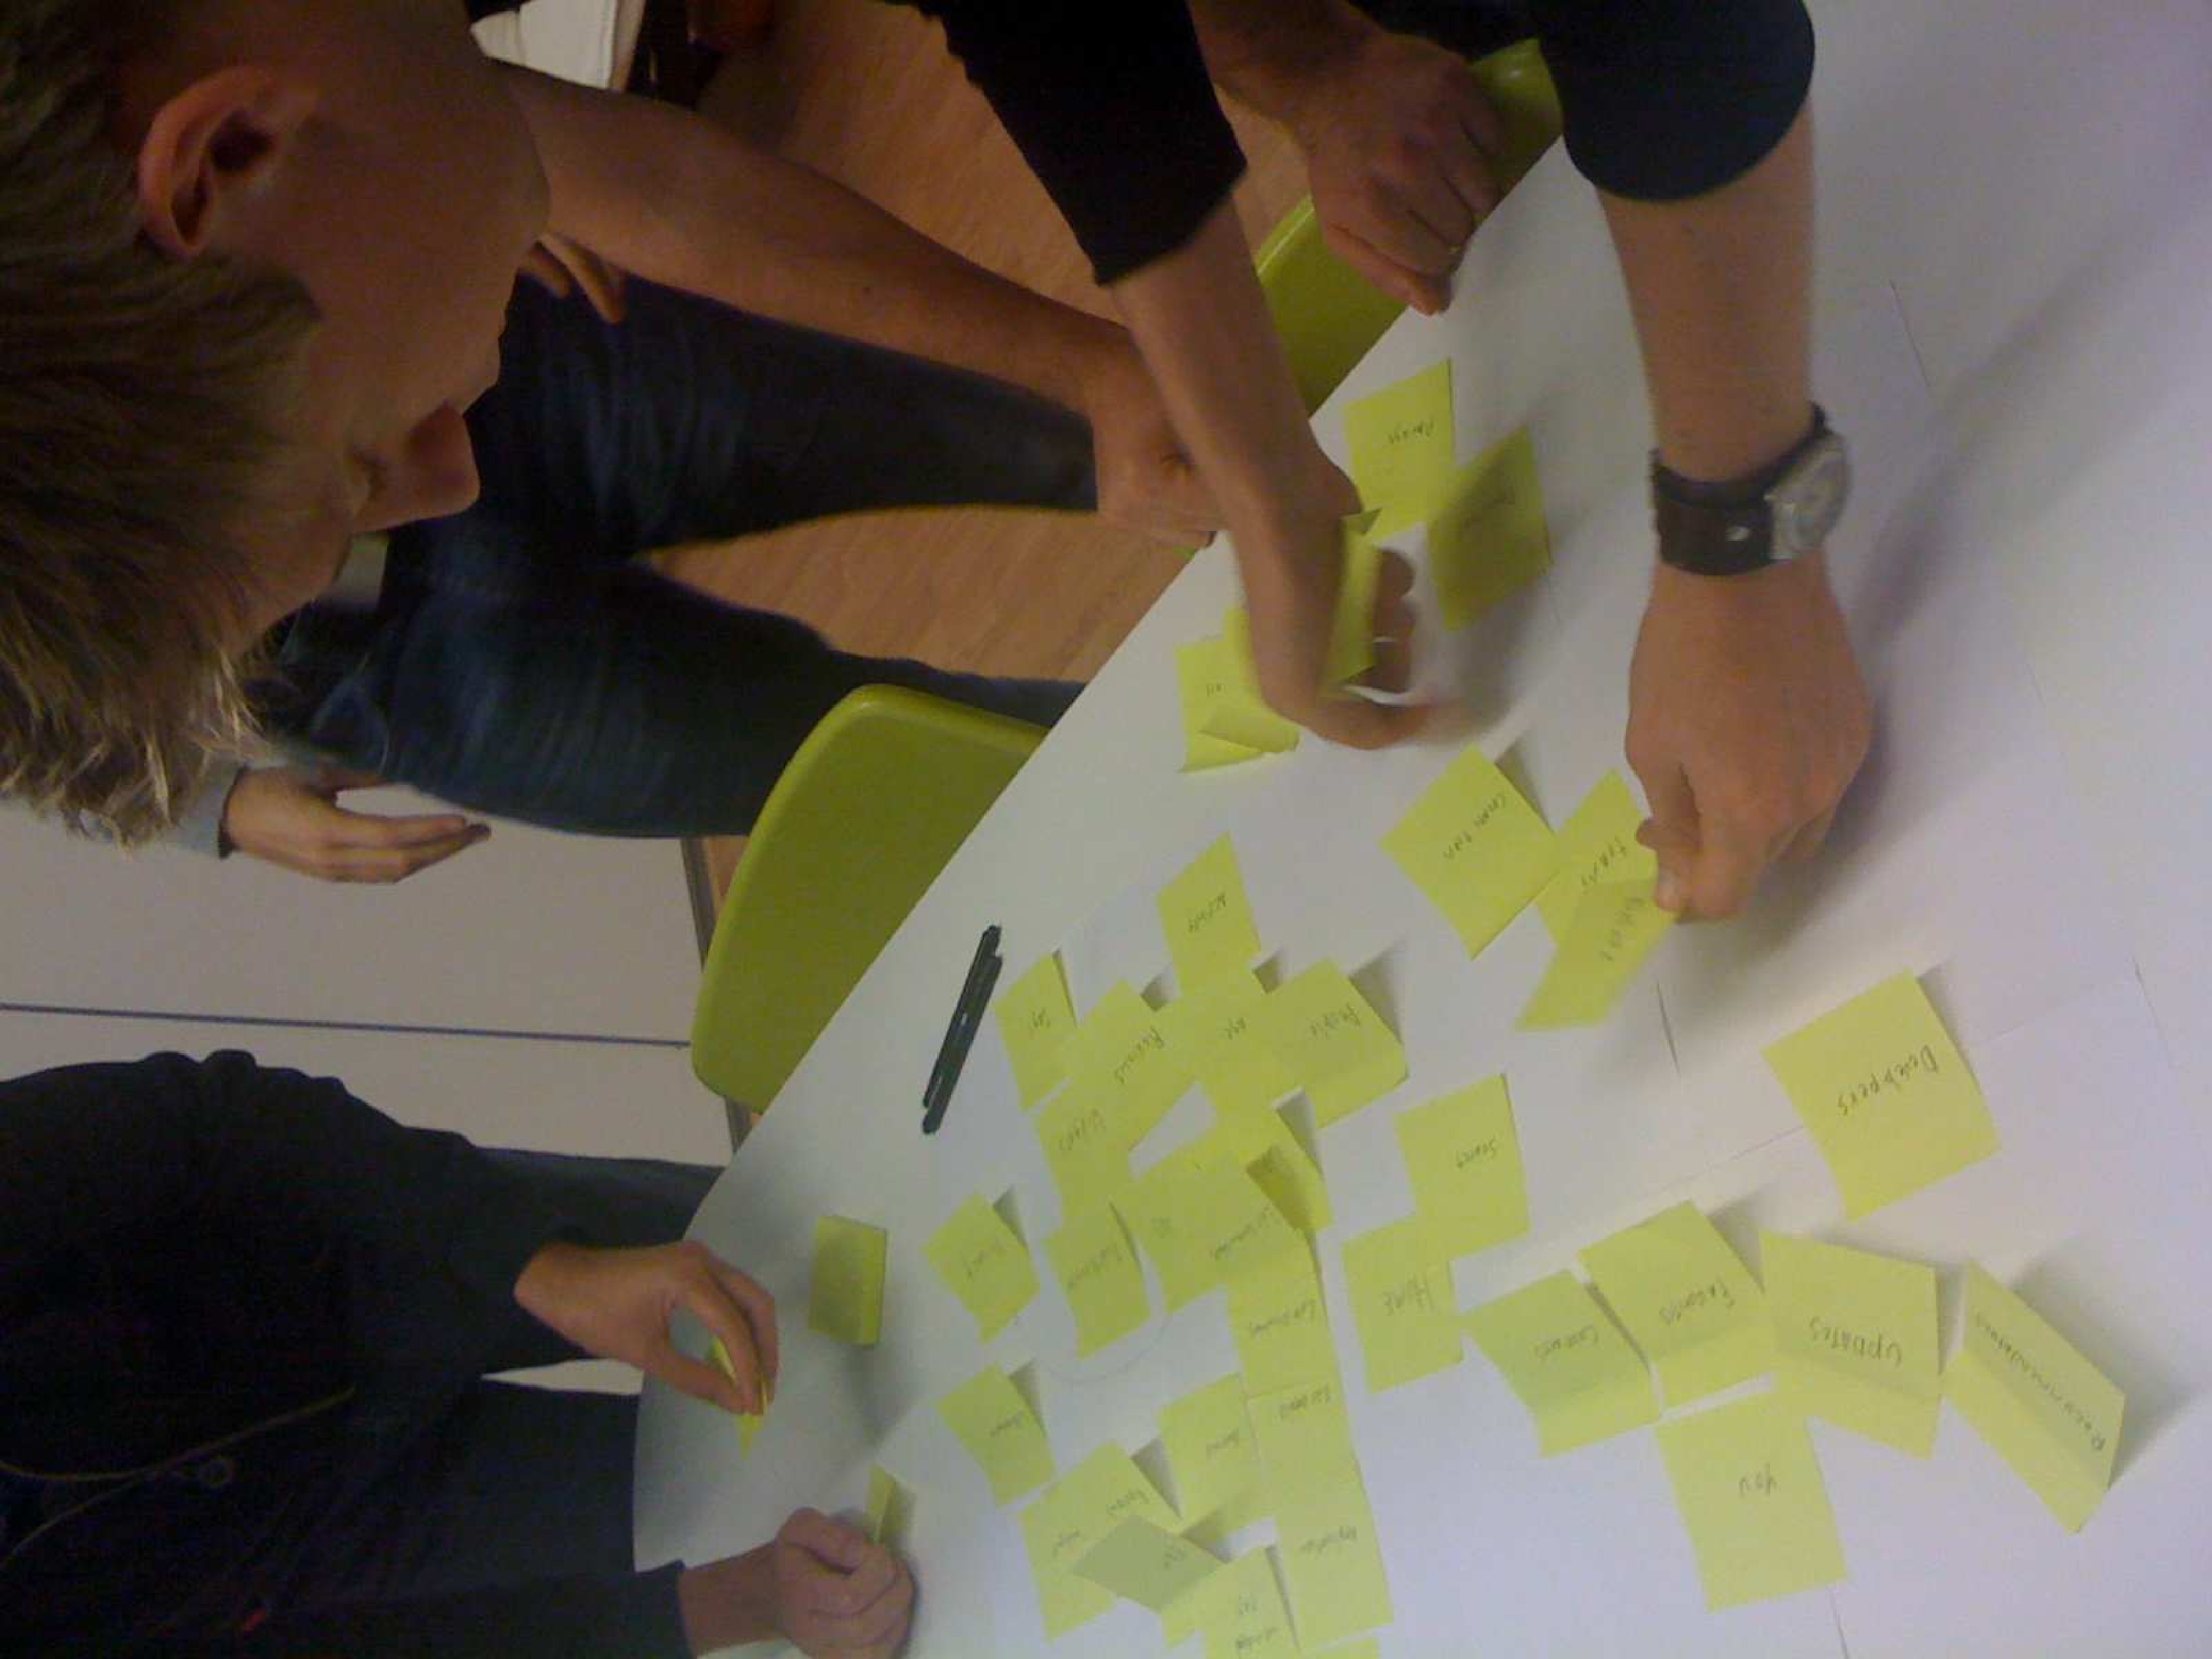
\includegraphics[height=6cm,angle=-90]{../images/navigatie-workshop/workshopimg1}}
        \subfigure{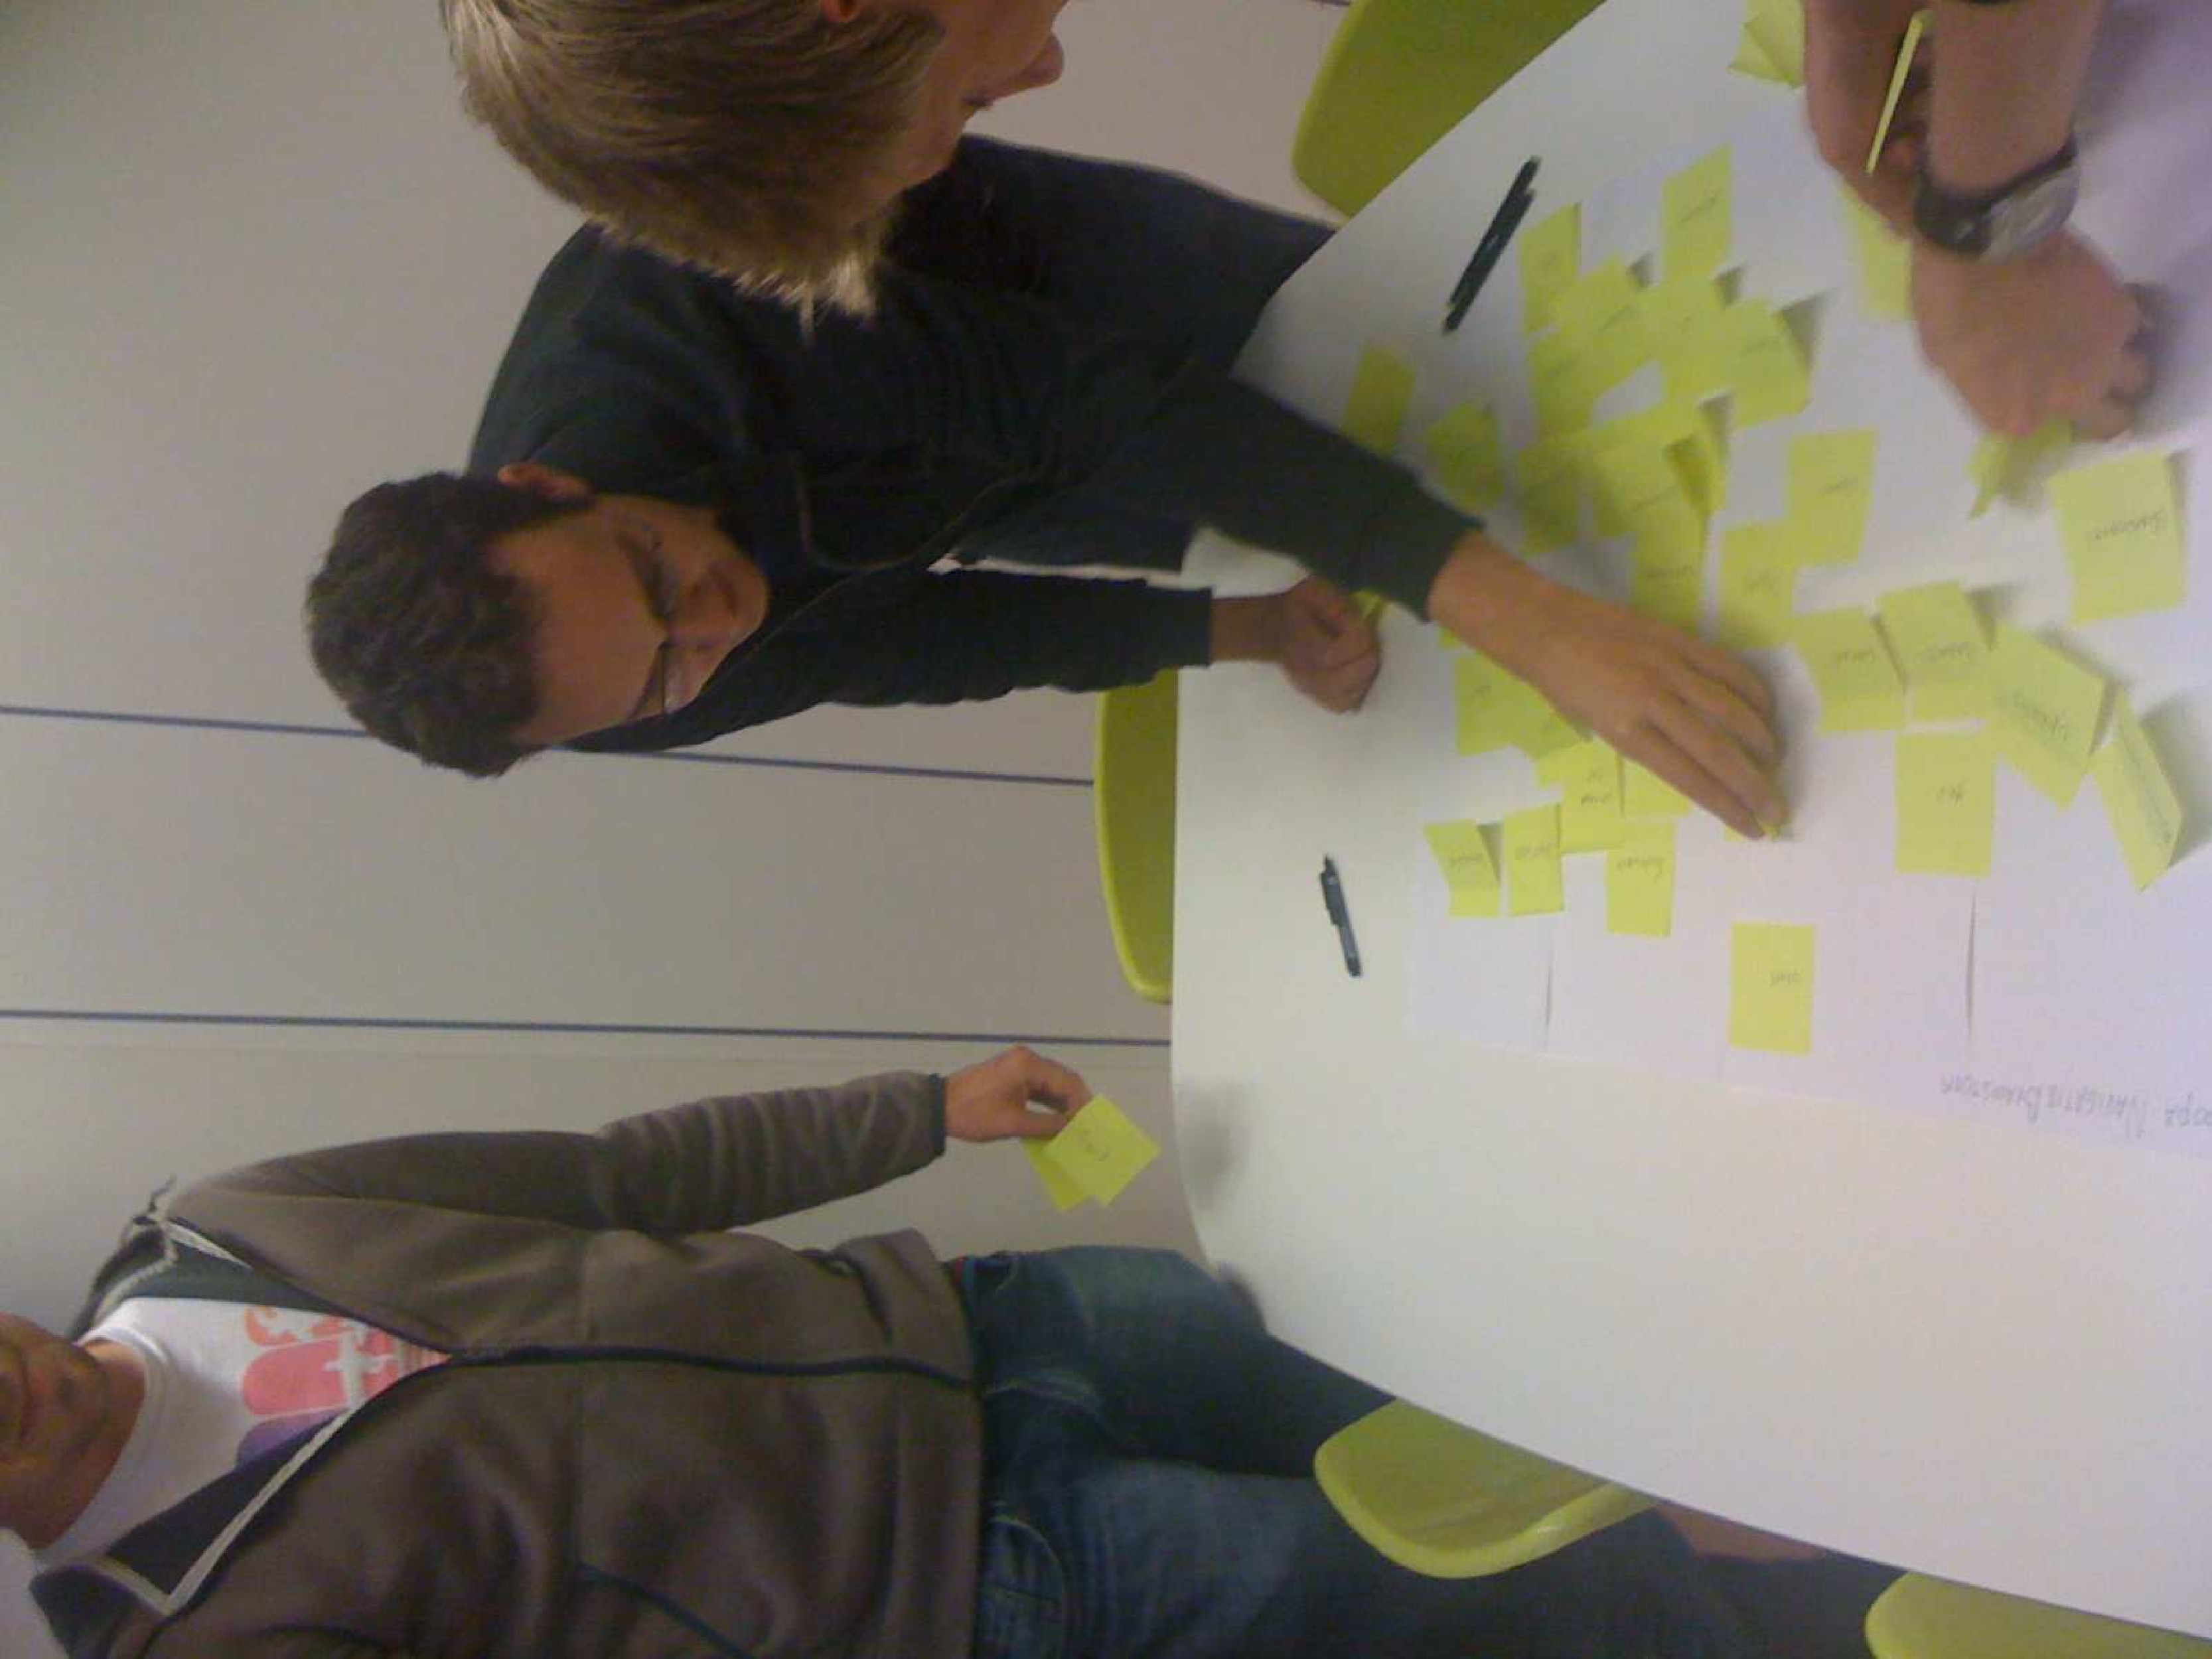
\includegraphics[height=6cm,angle=-90]{../images/navigatie-workshop/workshopimg3}}
        \subfigure{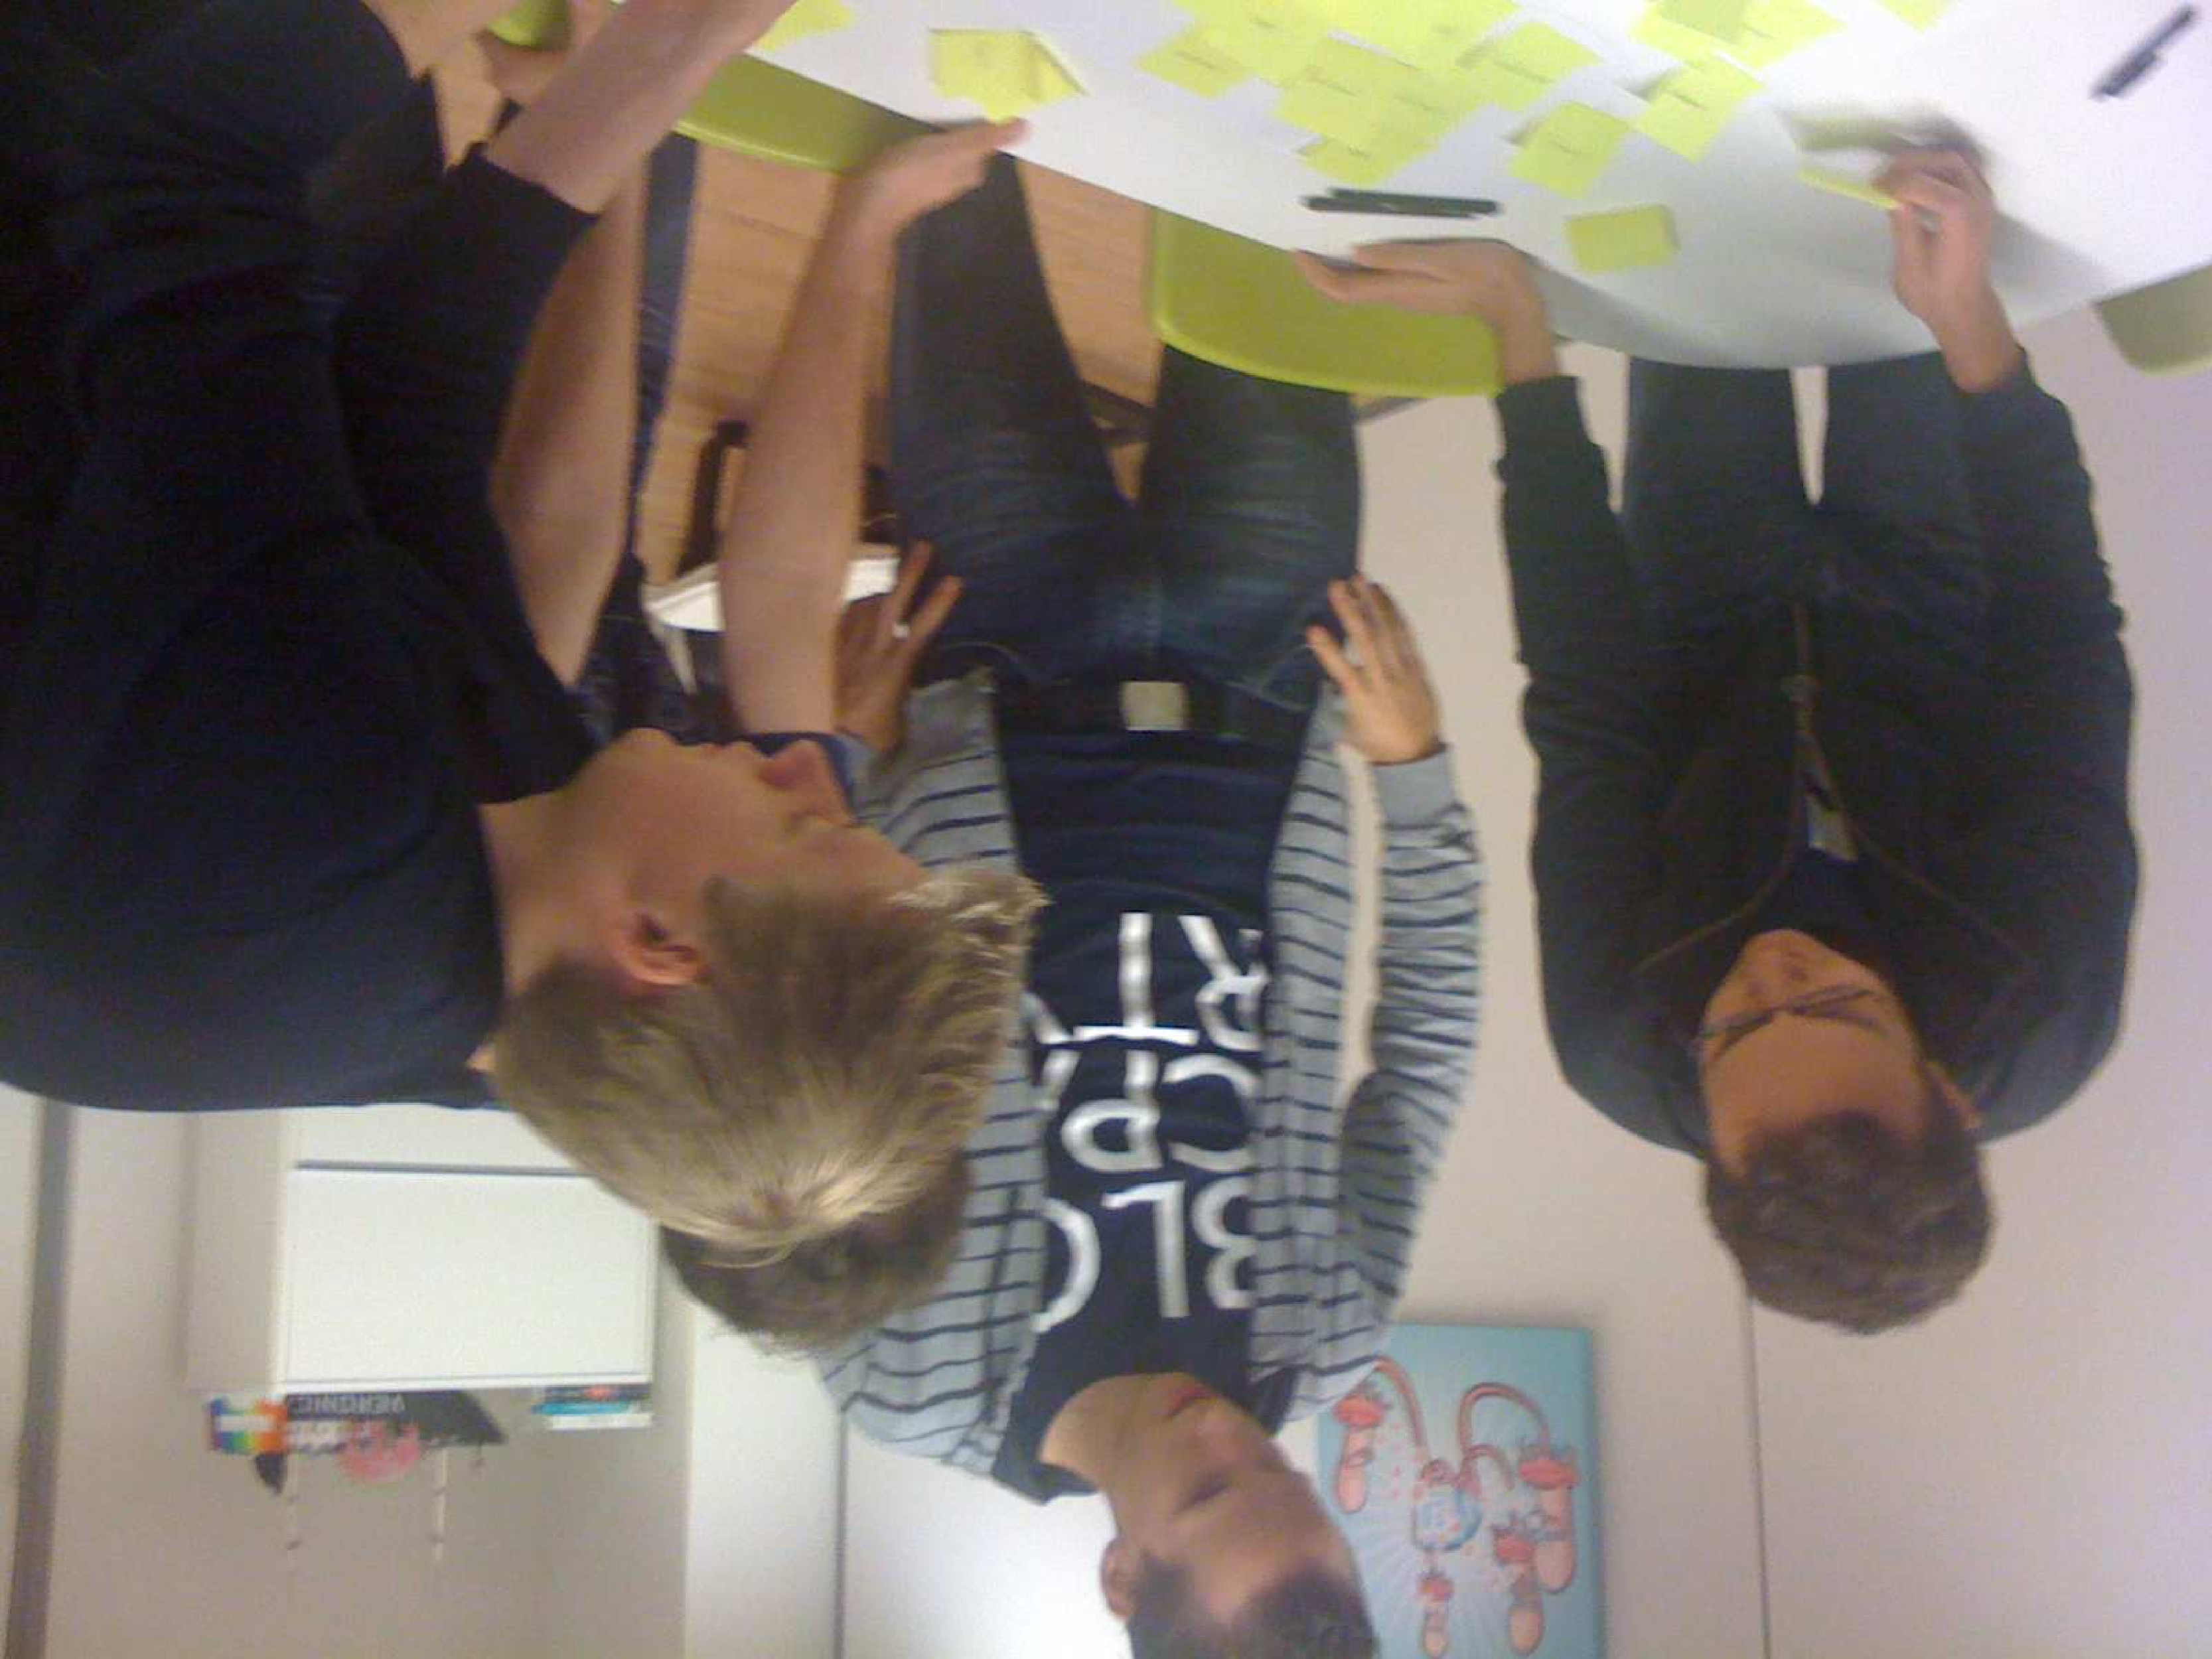
\includegraphics[height=4.5cm,angle=180]{../images/navigatie-workshop/workshopimg2}}
        \subfigure{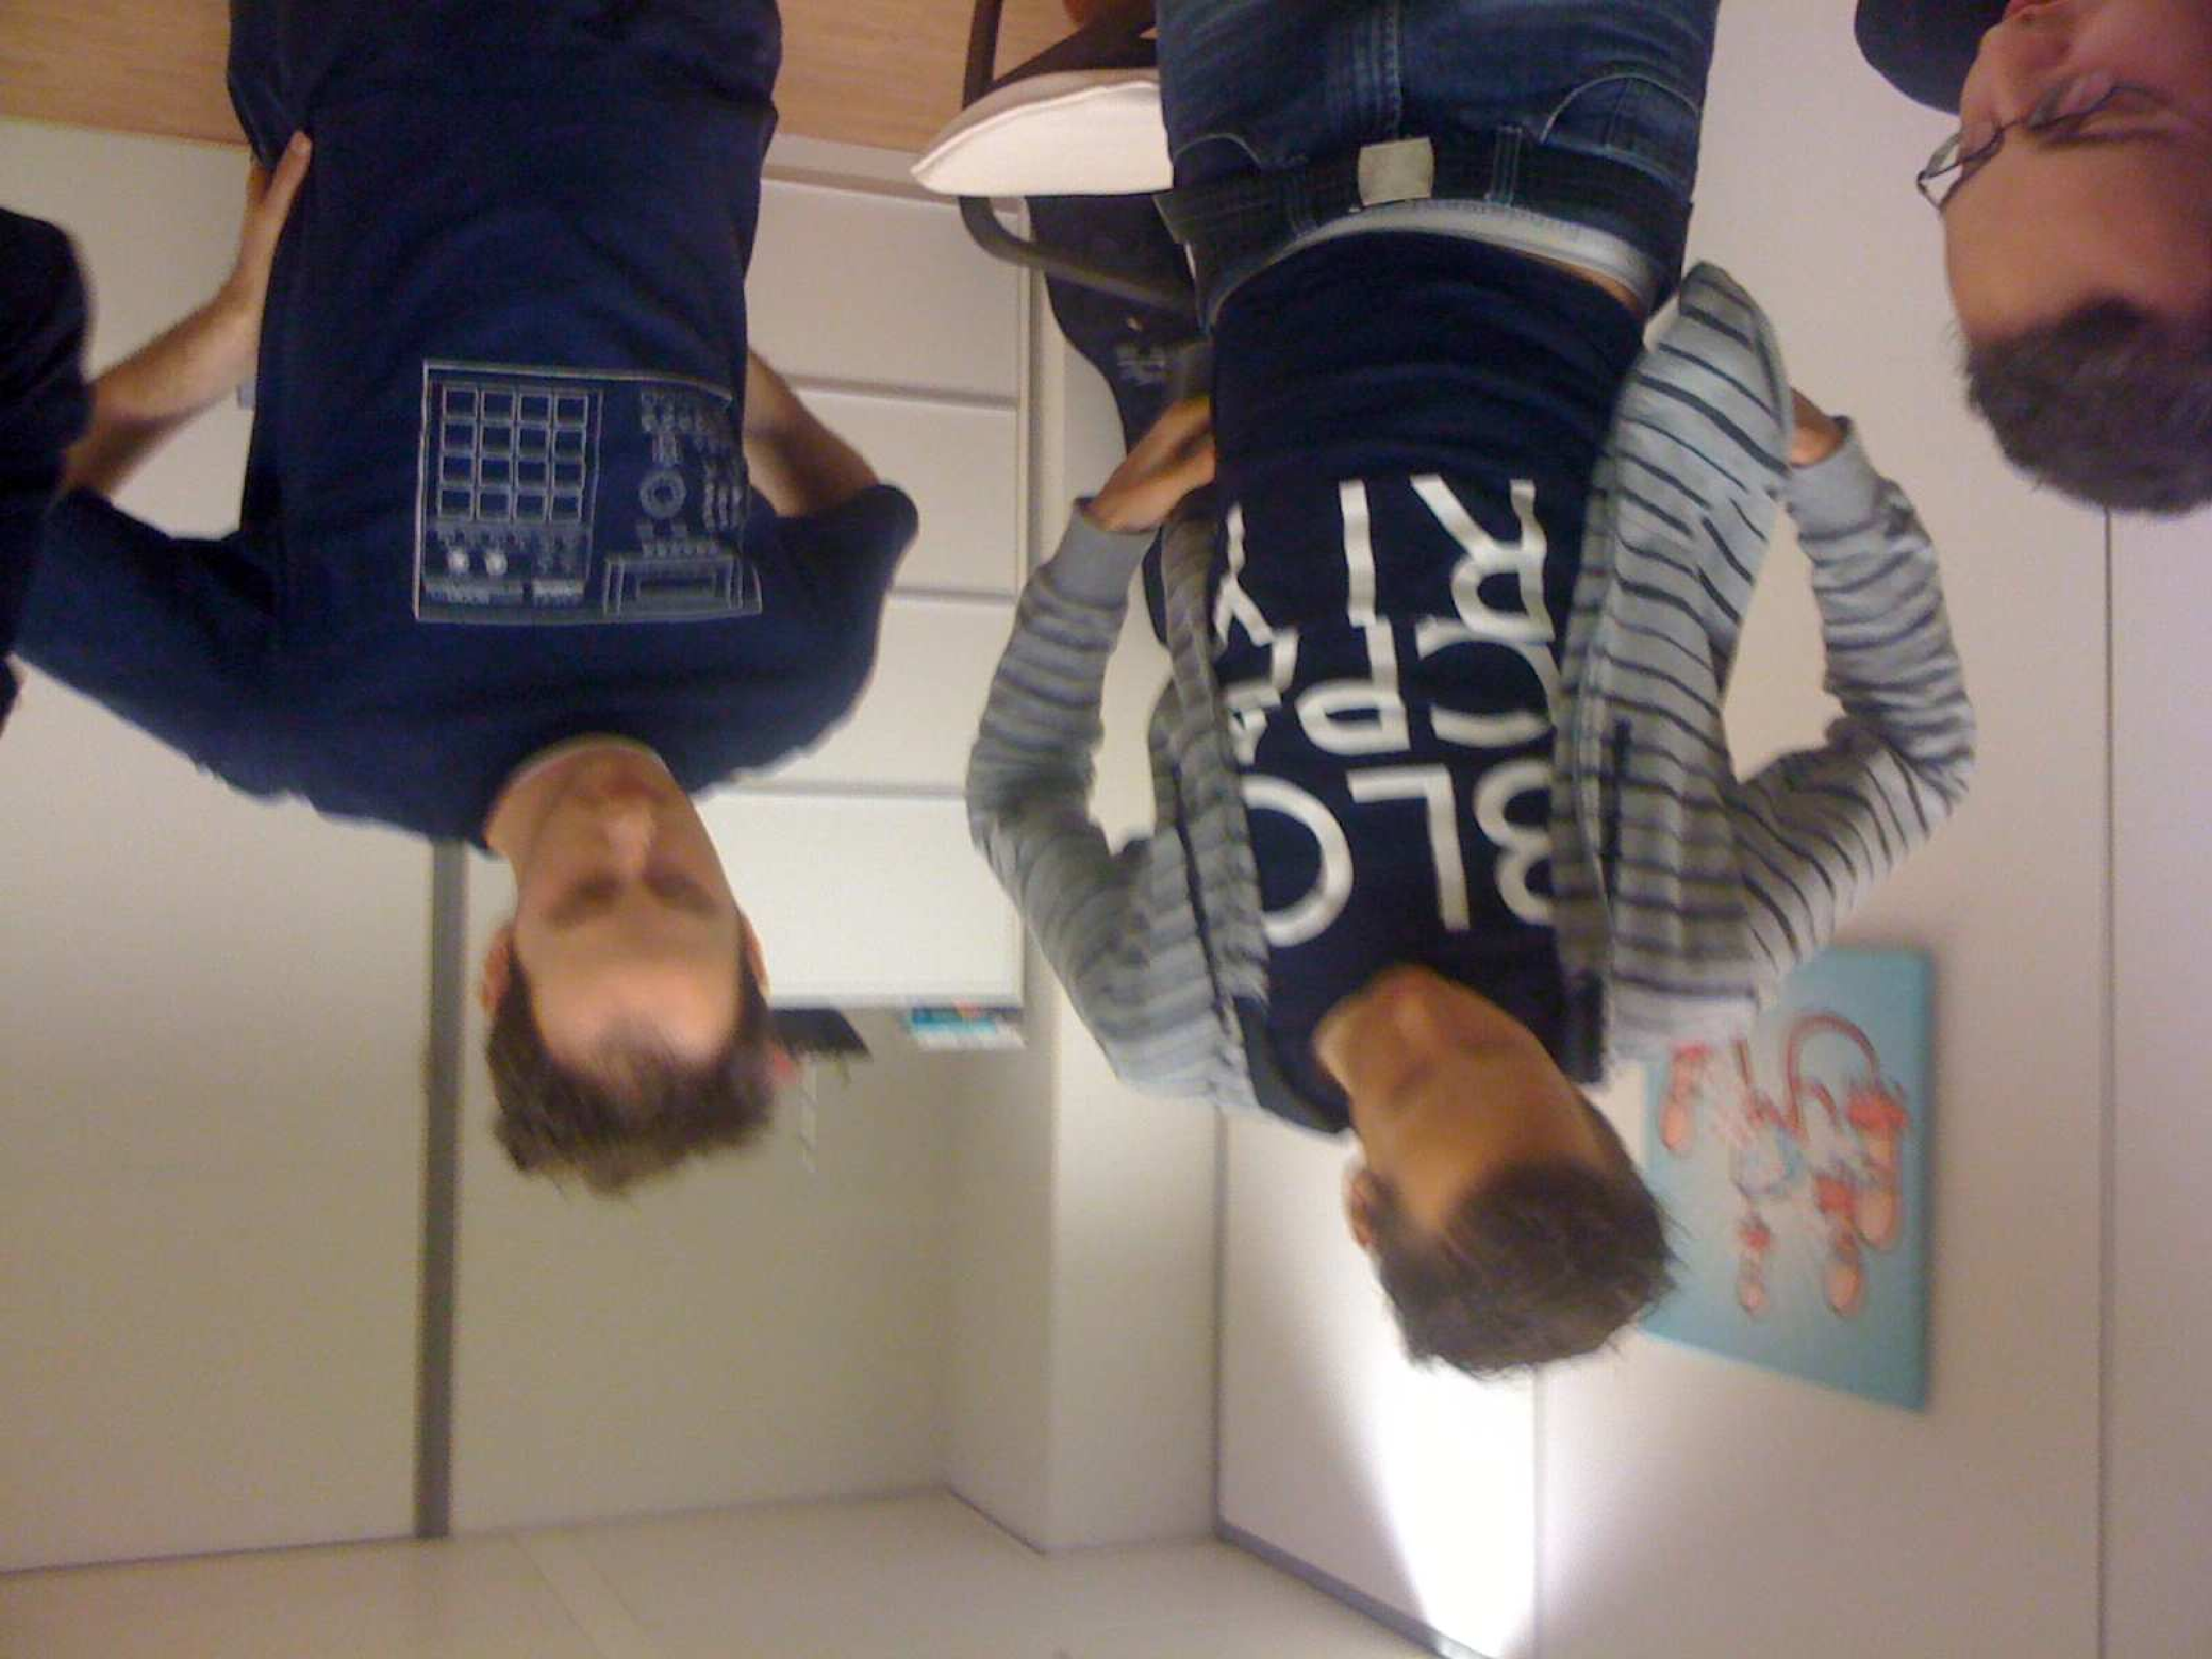
\includegraphics[height=4.5cm,angle=180]{../images/navigatie-workshop/workshopimg4}}
        \subfigure{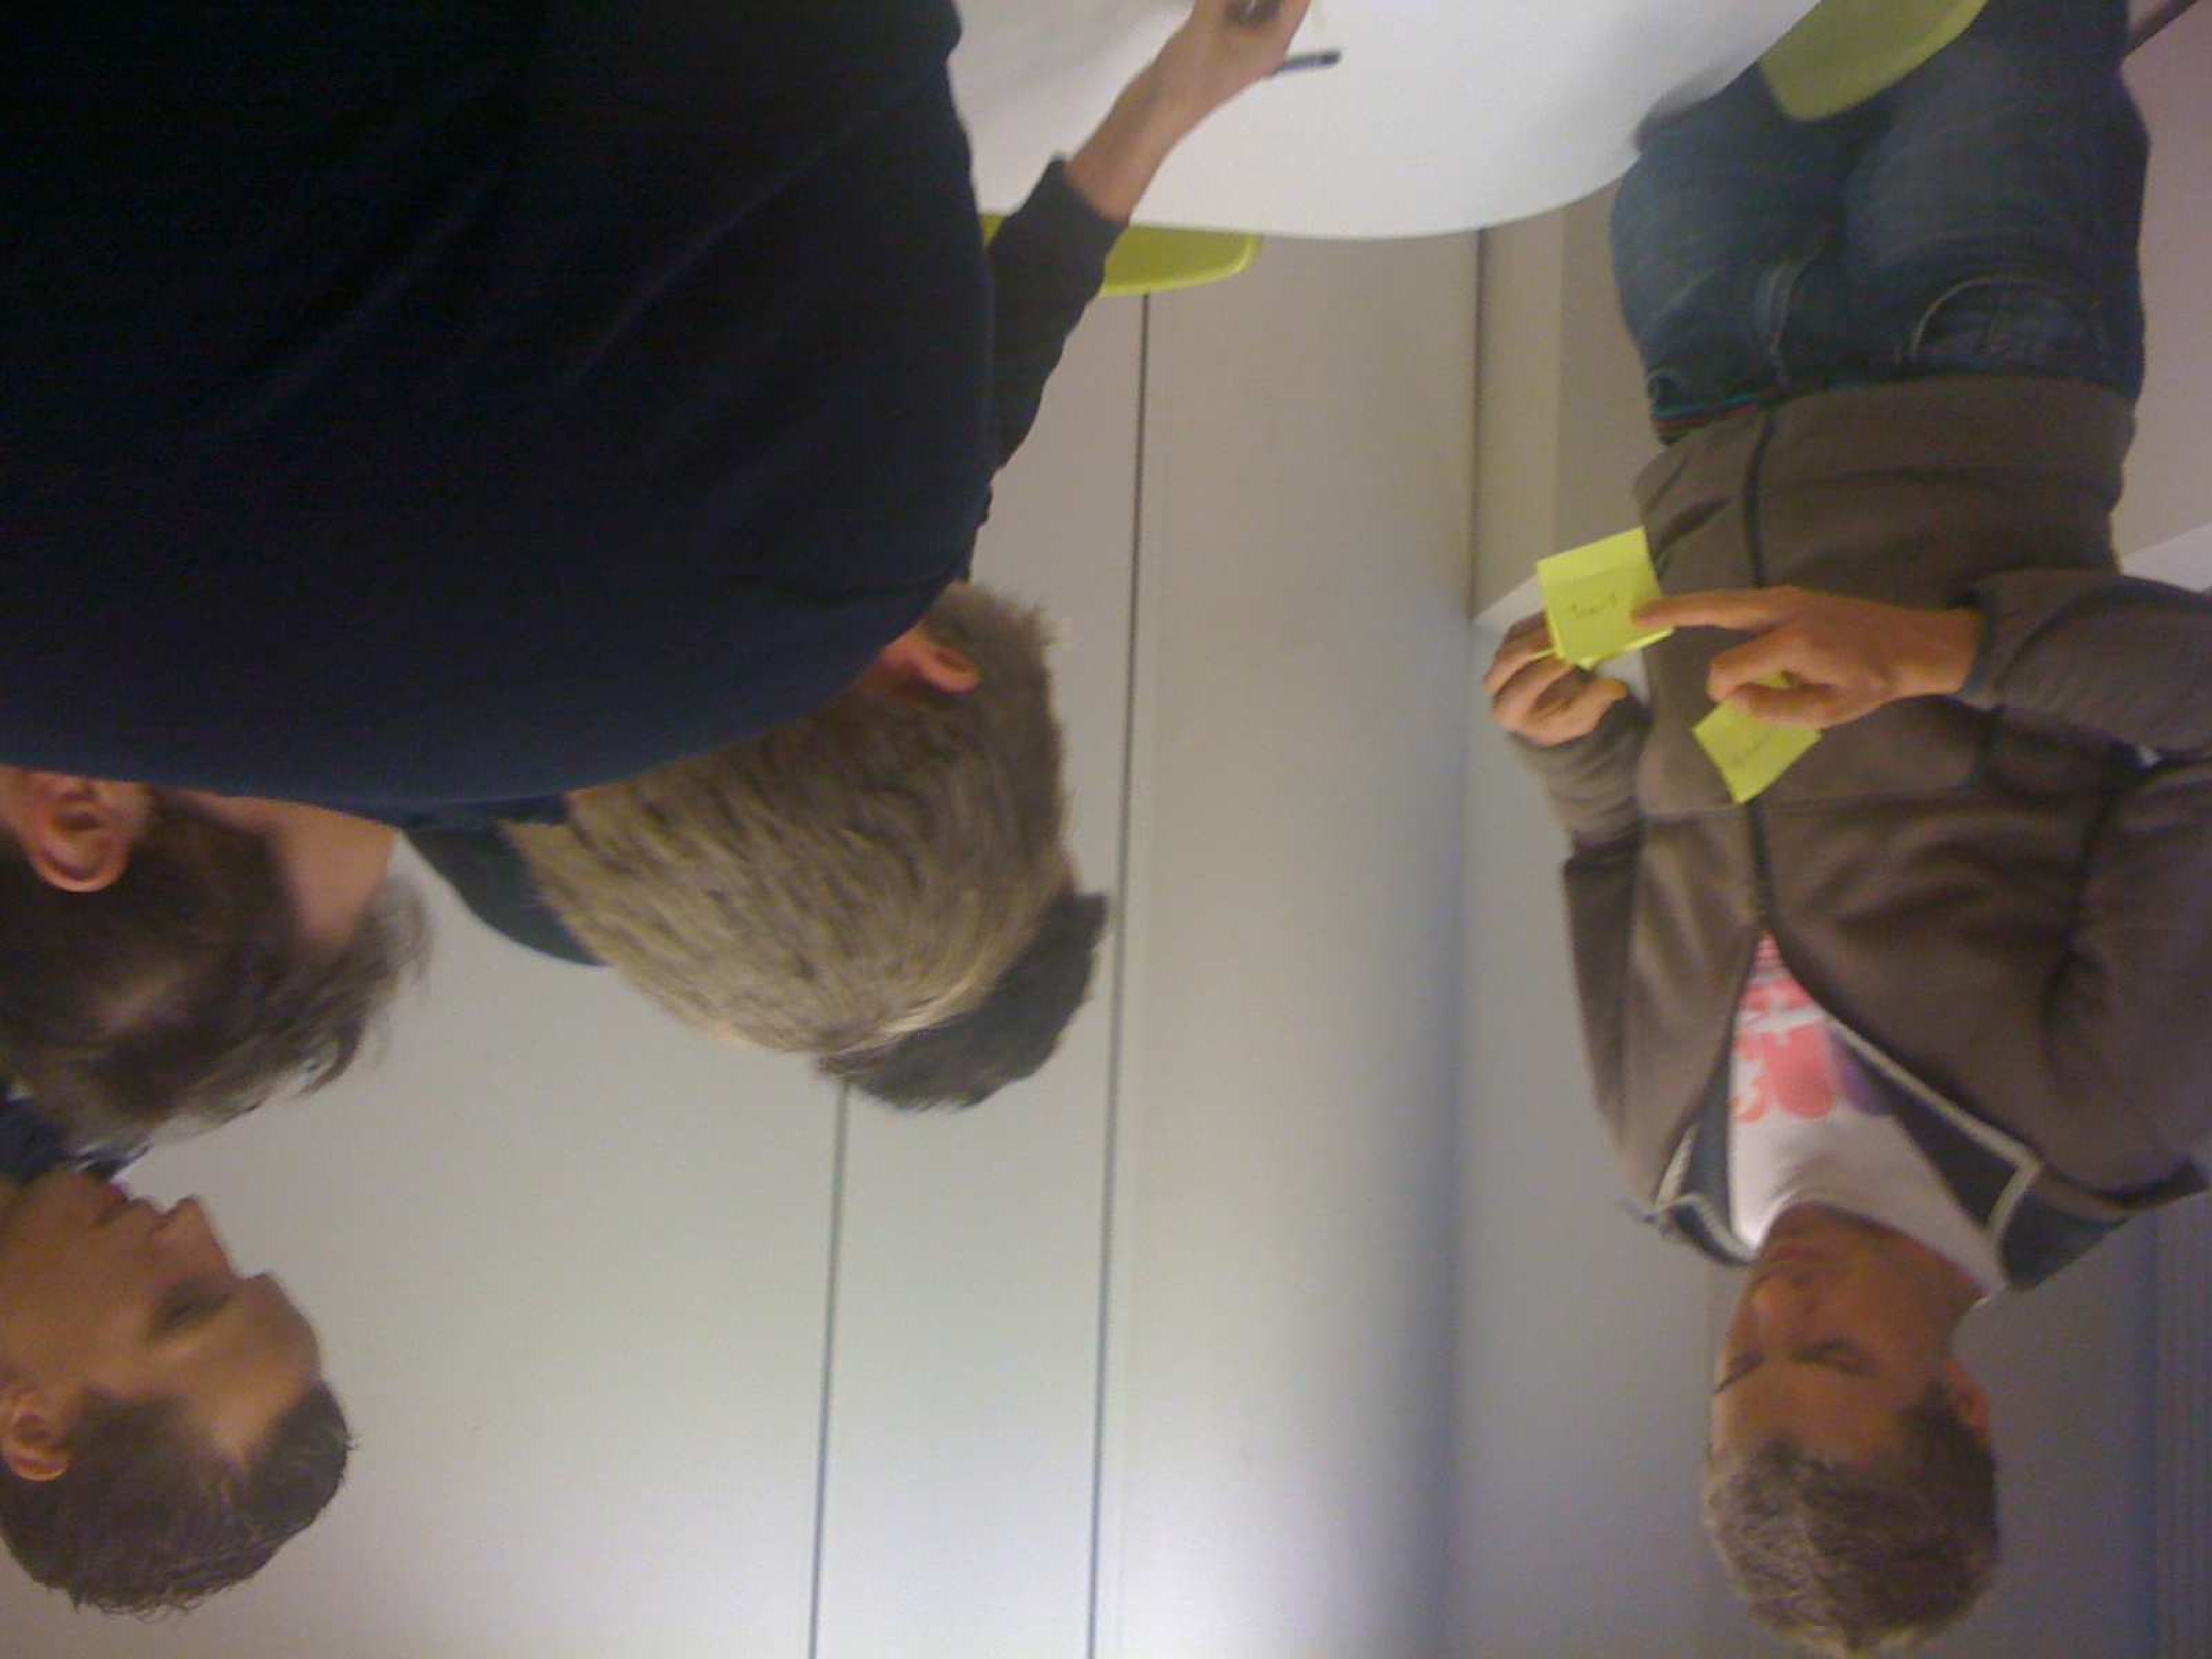
\includegraphics[height=4.5cm,angle=180]{../images/navigatie-workshop/workshopimg5}}
        \subfigure{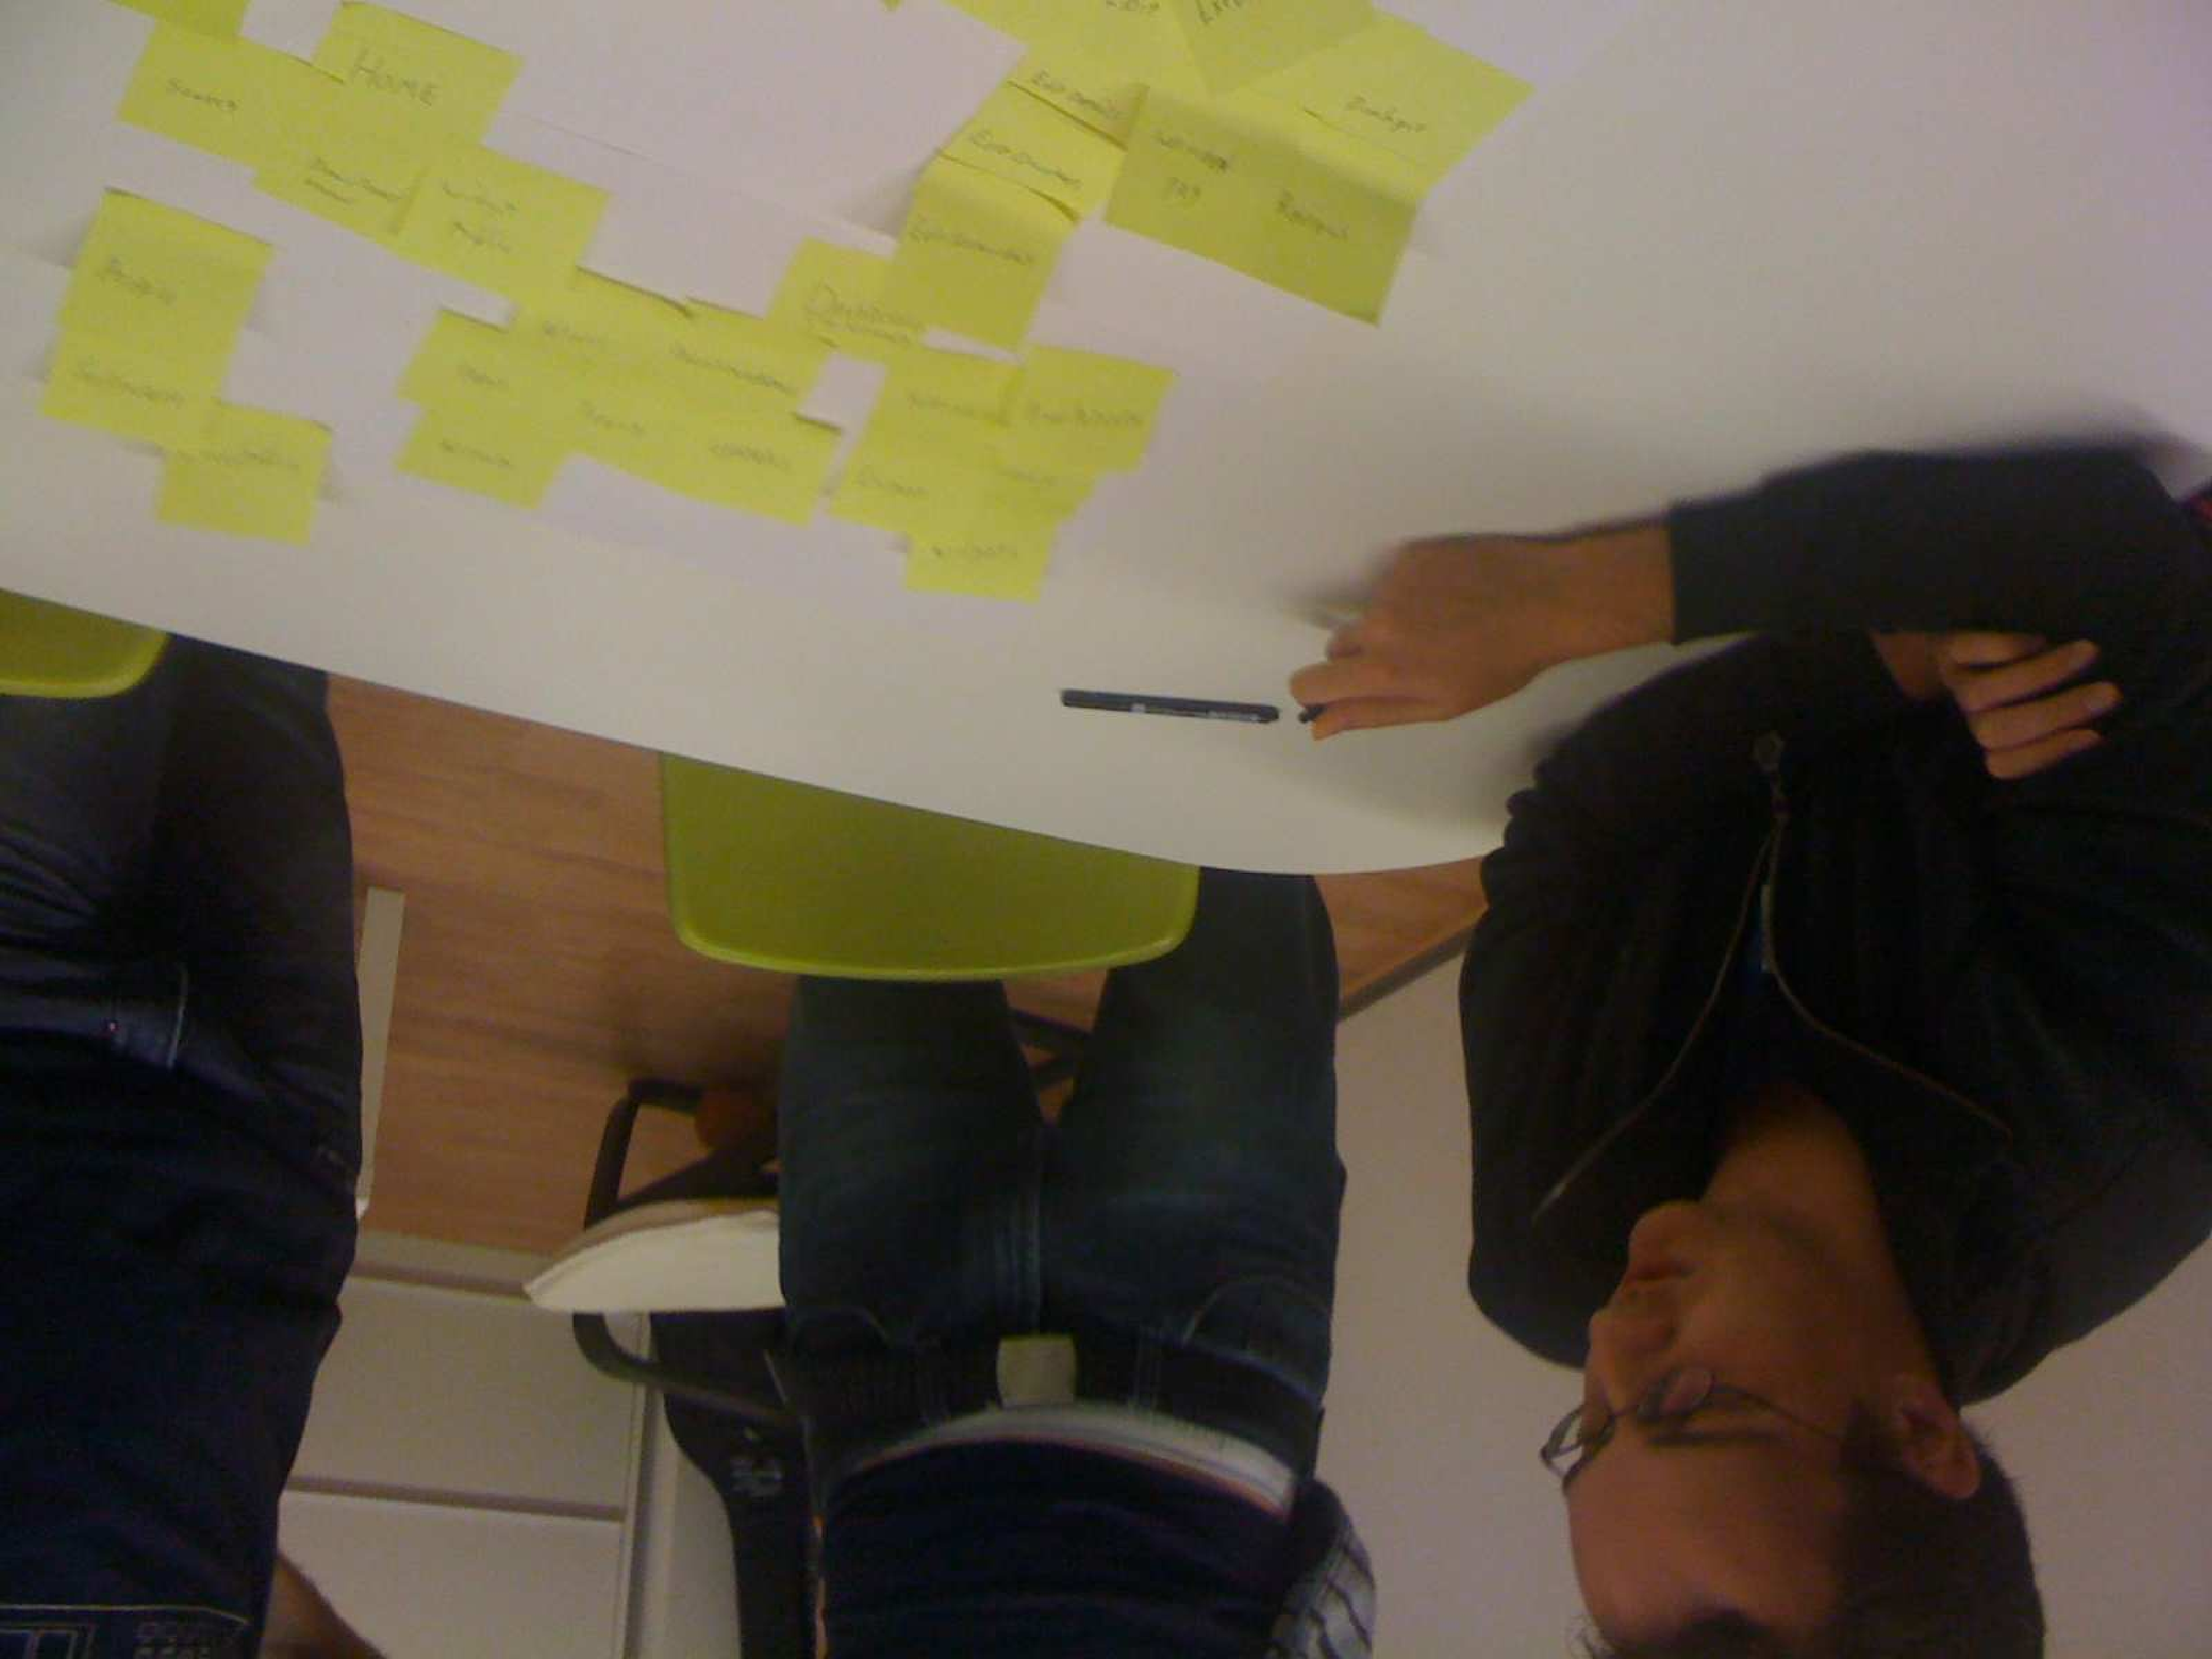
\includegraphics[height=4.5cm,angle=180]{../images/navigatie-workshop/workshopimg6}}
      \end{center}
    \end{figure}


    \label{navigationappendix}
  \chapter{Custom tracking items}
    \label{customtrackingappendix}
     De volgende items zullen worden getracked:
     \begin{itemize}
     \item vergroten van een screenshot
     \item bekijken van de category graph, periode dag
     \item bekijken van de category graph, periode week
     \item bekijken van de category graph, periode maand
     \item bekijken van de most used graph, periode dag
     \item bekijken van de most used graph, periode week
     \item bekijken van de most used graph, periode maand
     \item openen van de redenatie voor een aanbeveling
     \item het verwijderen van een aanbeveling
     \item het schrijven van een review
     \item zoeken via een ajax zoekveld
     \item openen van het favorite-toevoegen blok op een softwarepagina
     \item toevoegen van een favorite
     \item scrollen door gebruikers op een softwarepagina
     \item scrollen door screenshots op een softwarepagina
     \item openen van het tag-toevoegen blok op een softwarepagina
     \item toevoegen van een tag
     \item iemand toevoegen als contact
     \item verwijderen van een favorite
     \item openen van het privacy-settins blok op een softwarepagina
     \item verbergen van de intro promobar
     \item verzenden van een bericht via een reply
     \item verbergen van de promobar
     \item verbergen van de profile-completion bar
     \item laten zien van de software editing guidelines
     \end{itemize}


    \label{customtrackingappendix}
  \chapter{Enqu\^ete}
      \section{Demografie}
        Om te kijken in hoeverre de enqu\^ete de mening van alle Wakoopa leden vertegenwoordigd, is het belangrijk om te kijken of de demografie van de twee overeenkomen.De demografie van de respondenten is te vinden in figuren \ref{fig:gender}, \ref{fig:country} en \ref{fig:age}. Qua leeftijd, geslacht en land verschilt dit slechts een aantal procenten met de demografie van Wakoopagebruikers. De enqu\^ete, met 1069 respondenten, is daarom een goede graadmeter van de mening van Wakoopaleden.
        \begin{figure}
          \begin{center}
          \caption{Geslacht van respondenten}
            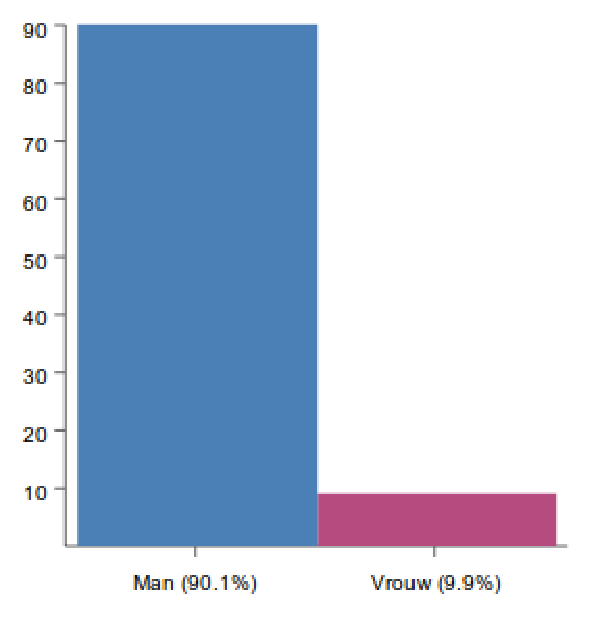
\includegraphics[height=60mm, angle=90]{../images/enquete/gender}
          \label{fig:gender}

          \caption{Land van afkomst van respondenten}
            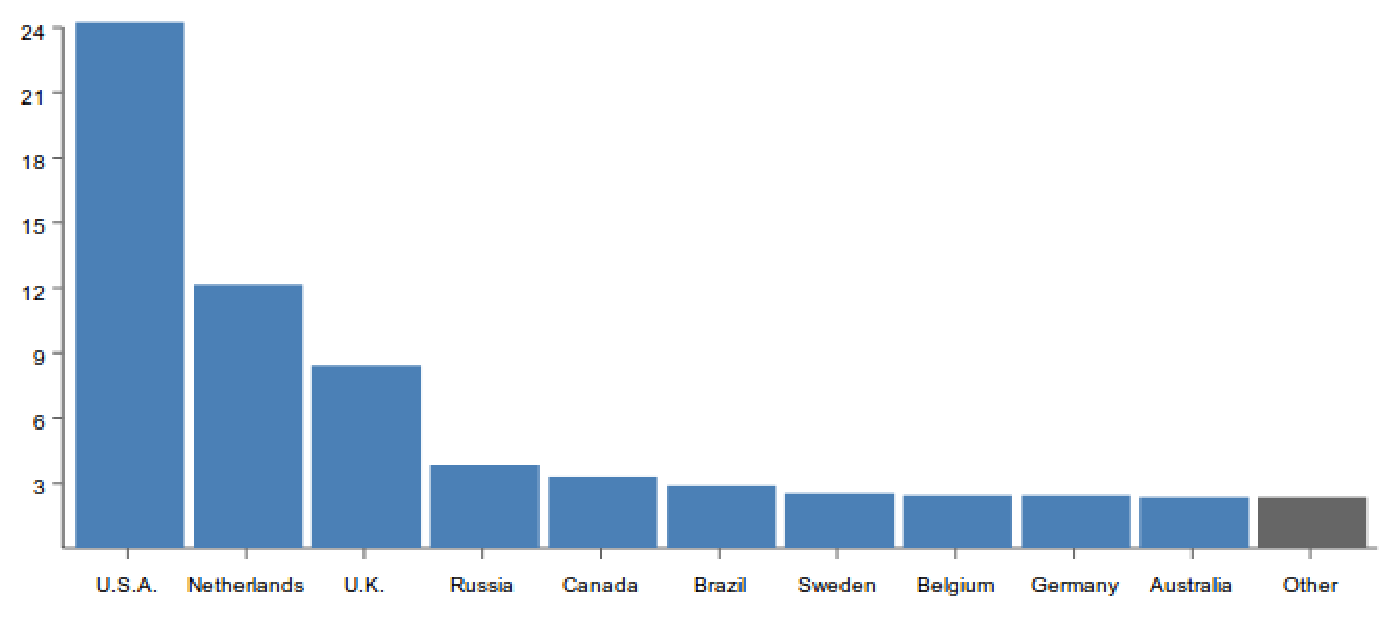
\includegraphics[height=60mm, angle=90]{../images/enquete/country}
            \label{fig:country}

          \end{center}
        \end{figure}

        \begin{figure}
          \begin{center}
          \caption{Leeftijd van respondenten}
            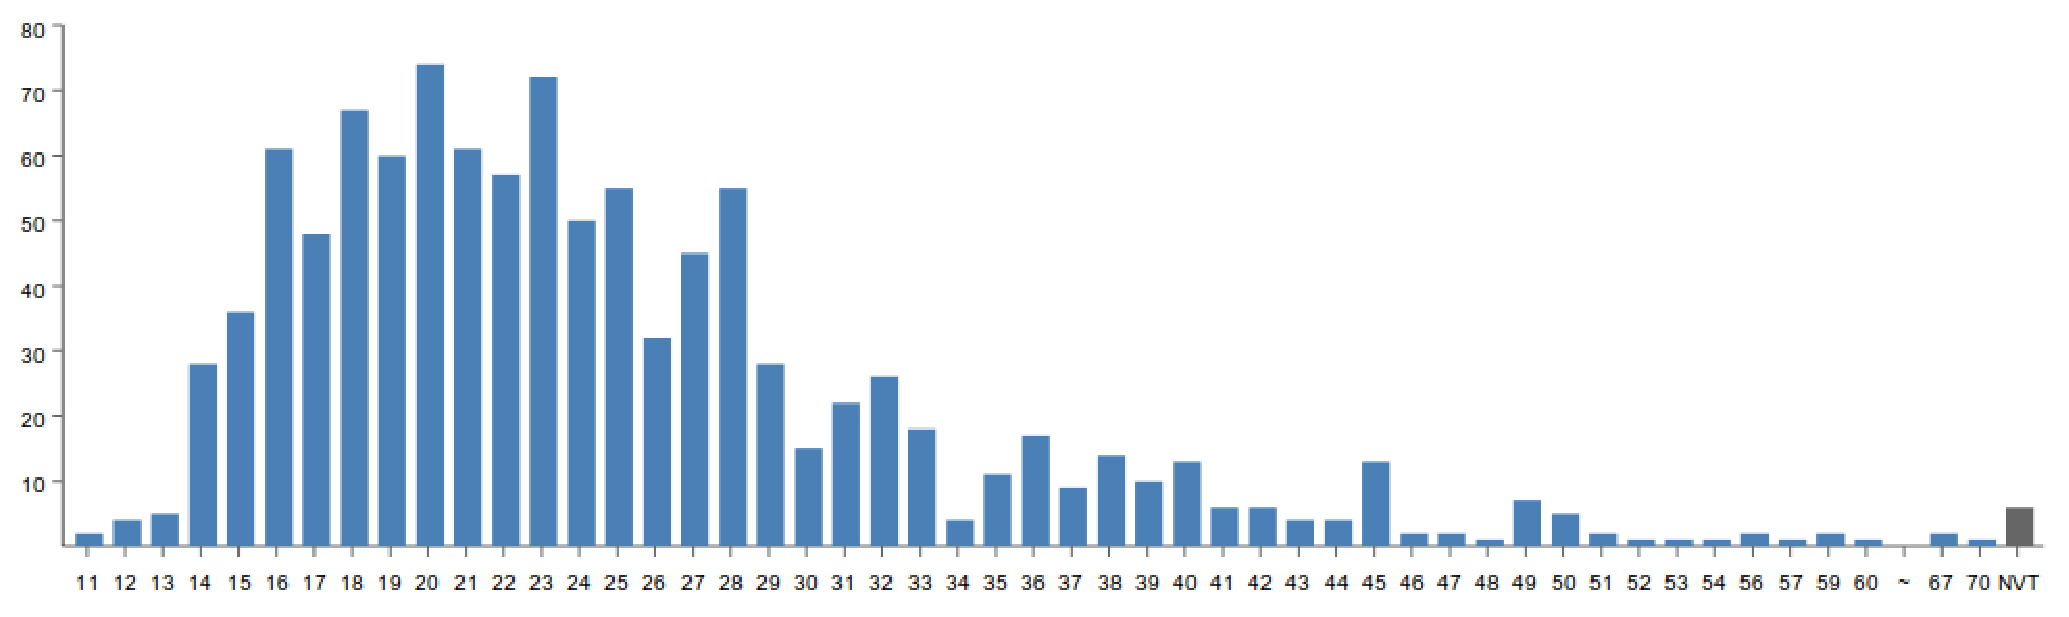
\includegraphics[height=58mm, angle=90]{../images/enquete/age}
          \label{fig:age}

          \end{center}
        \end{figure}

      \section{Bevindingen}
        De enqu\^ete ging verder met vragen naar hoe kundig de respondenten met computers waren (Figuur \ref{fig:skill}). Het overgrote deel (49.2\%) van de respondenten vind zichzelf \emph{excellent} op computergebied. een klein percentage vind zichzelf een novice (0.3\%) of classificeerd zichzelf als `lerende' (1.5\%). Eenentwintig procent acht zichzelf in het midden met `pretty good'. Als laatste is achtentwintig procent van de respondenten zelf actief bezig met het ontwikkelen van applicaties. Uit deze uitkomst is op te maken dat zich onder de respondenten een hoog percentage experts, of zogenaamde "power users", bevinden.
        \begin{figure}
          \begin{center}
          \caption{Kundigheid met computers}
            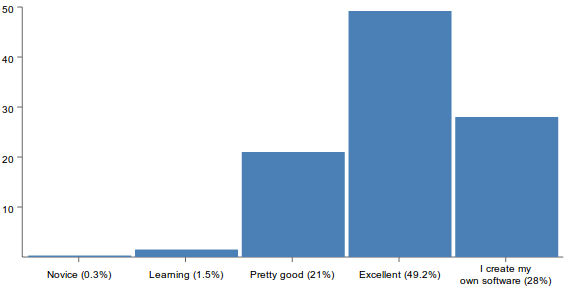
\includegraphics[height=50mm]{../images/enquete/good-with-computers}
          \label{fig:skill}
          \end{center}
        \end{figure}

      In Figuur \ref{fig:visit-website} werd de vraag gestelt hoe vaak gebruikers de Wakoopa site bezochten en er werd gevraagd waarom ze met dit interval de site bekeken. Het overgrote deel van de respondenten bekeek, met 43.1\%, de site wekelijks, gevolgd door een derde van de respondenten die dagelijks keek. Een greep uit de gegeven redenen:
        \begin{figure}
          \begin{center}
          \caption{Hoe vaak wordt de website bezocht?}
            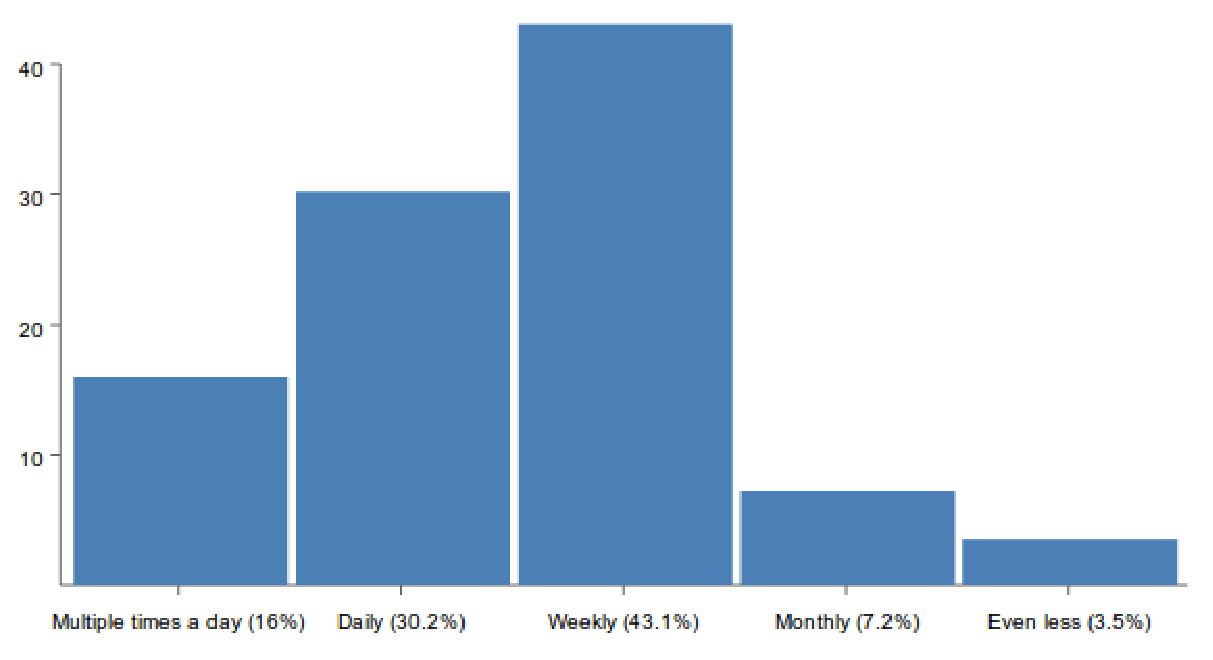
\includegraphics[height=50mm]{../images/enquete/visit-website}
          \label{fig:visit-website}
          \end{center}
        \end{figure}

      \paragraph{Wekelijk (43.1\%)}
        \begin{itemize}
          \item Because of the weekly summary mail
          \item Because that is when I get my summary
          \item I need some weekly reports about my software and timetracking reports.
          \item To see the "big" changes is my software behaviour. And to see if there is new software i could try out.
        \end{itemize}

      \paragraph{Dagelijks (30.2\%)}
        \begin{itemize}
          \item It's interesting to see all the data and usage stuff.
          \item To check what level I am. Always seeking to level up..!
          \item To check out what new software is out there \& it's cool to see what my habits are on my Mac.
          \item Check my profile stats
        \end{itemize}

      \paragraph{Meerdere malen per dag (16\%)}
        \begin{itemize}
          \item To see how many points i'm earning, and to just snoop on other peoples profiles. you know, creep. like on facebook. but the people here are more interesting than my facebook people :)
          \item Well, the system tray icon keeps notifying me the new activities
          \item To see how my friends are doing and me, and so I can win in the battle of using the most software in less time. :)
          \item Because I love statistics, I find it rewarding to see figures and graphs about something I accomplished! that's the reason why I'm also a last.fm and whatpulse addict. and apart from that, I really like software (especially freeware) and like to see suggestions for other software.
        \end{itemize}

      \paragraph{Maandelijks (7.2\%)}
        \begin{itemize}
          \item There's no need to use it more often
          \item Because I got an update.
          \item I like to see my stats and get new ideas on software/sites.
          \item I only check the site when I am looking for alternative software or I see something I like in the newsletter.
        \end{itemize}

      \paragraph{Minder dan maandelijks (3.5\%)}
        \begin{itemize}
          \item I'm still waiting for the linux app
          \item Nothing of tons of interest on site, just as often as I visit Last.FM It is useful when uninstalling things.
          \item Because I use Linux, I am waiting for a Linux tracker. Without it, Wakoopa is just another computer-oriented forum to me.
        \end{itemize}

      \paragraph{}Zoals uit de verschillende gegeven redenen op te merken is, is er een relatie tussen hoe vaak mensen de site bezoeken en hoe enthousiast ze er over zijn. Onder wekelijkse bezoekers is het aantal wat aangeeft de website te bezoeken na het ontvangen van de wekelijkse mail het hoogst. De mensen die een of meerdere malen per dag de site bekijken, zijn er voornamelijk voor de grafieken, statistieken en punten. Omgekeerd, de respondenten die slechts maandelijks of minder de site bekijken, zeggen dat ze dit doen omdat er niet genoeg nieuws of informatie op de site staat om deze vaker te bezoeken.

        \begin{figure}
          \begin{center}
          \caption{over welke nieuwe functionaliteit ben je het meest enthousiast?}
            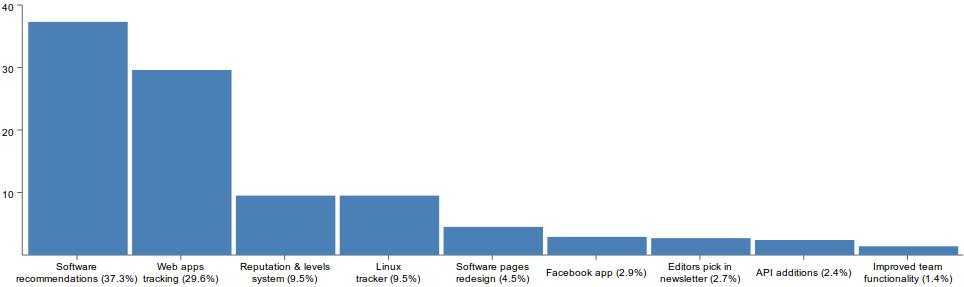
\includegraphics[width=\textwidth]{../images/enquete/recent-additions}
          \label{fig:enthousiast}
          \end{center}
        \end{figure}

      Een learning network is vaak bezig met het ontwikkelen en online plaatsen van nieuwe functionaliteit. Het belangrijk om bij te houden wat de impact hiervan op de gebruikers is. Om dit te onderzoeken vroegen we in figuur \ref{fig:enthousiast} aan de respondenten welke recente toevoeging ze het meest enthousiast over waren. Met 37.3\% zijn de respondenten het meest enthousiast over de software aanbevelingen, kort daarop gevolgd door het tracken van web apps met 29.6\%. De eerstvolgende zijn respectievelijk het level-systeem en de linux tracker met beide 9.5\%.

        \begin{figure}
          \begin{center}
          \caption{Waar komt Wakoopa tekort?}
            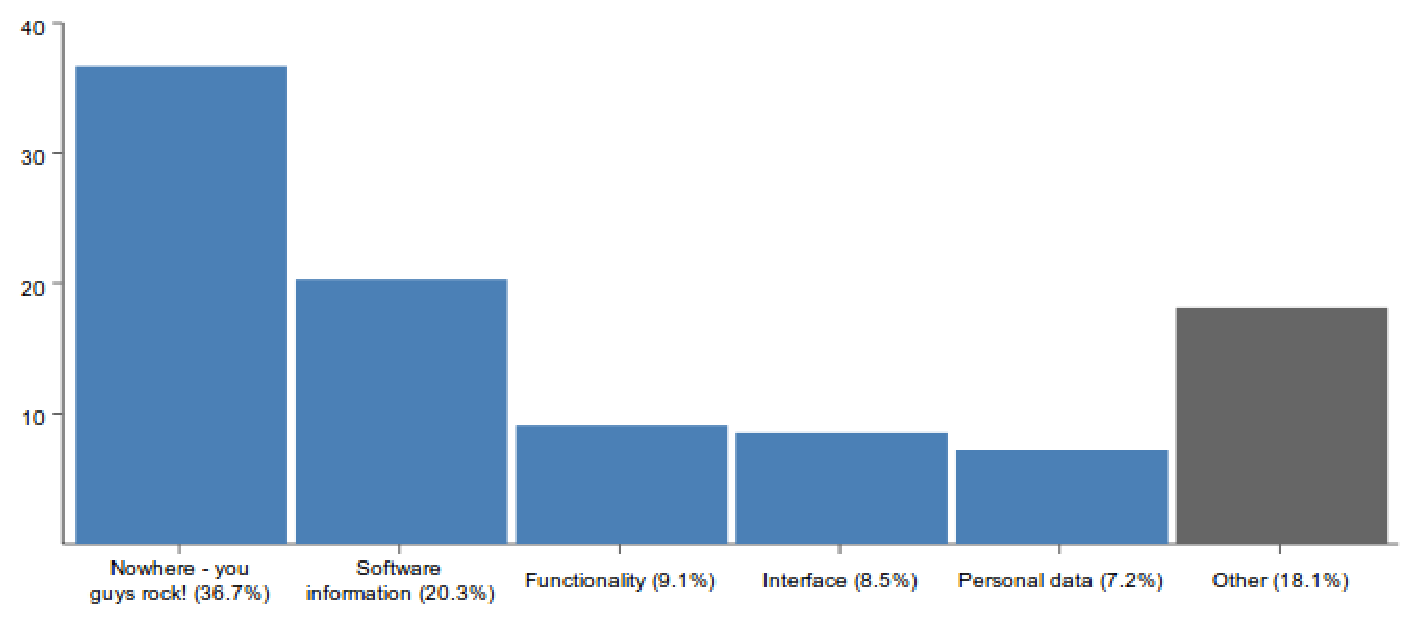
\includegraphics[width=\textwidth]{../images/enquete/improvement}
          \label{fig:improvement}
          \end{center}
        \end{figure}

      Minstens even belangrijk als weten waar mensen enthousiast over zijn is weten waar ze graag verbetering willen zien. Daarom stelde de enqu\^ete de vraag waar de respondenten Wakoopa nog in vonden tekortkomen. De respons hierop is te vinden in figuur \ref{fig:improvement}. Het meest gekozen antwoord was "Nowhere, you guys rock!". 36.7\% van de respondenten had geen grote problemen, of kon er niet direct een noemen. Hoewel dit positief is, zit de waarde van de vraag meer in de andere antwoorden.

      Een groot deel van de respondenten, 20.3\%, vind dat de informatie rondom software te wensen overlaat. Een kijk in het help-forum laat zien dat er inderdaad veel mensen toevoegingen aandragen op dit gebied.\footnote{\url{http://getsatisfaction.com/wakoopa/searches?query=software+information&style=topics}, geraadpleegd op 13 oktober 2009} Wat vaak voorkomt zijn vragen over meer informatie qua versies. Een recente ontwikkeling op dit gebied is dat softwareontwikkelaars nu hun versies en downloads op Wakoopa kunnen beheren, en voor een hogere kwaliteit van informatie kunnen zorgen.

      Een ander veelvoorkomend punt is dat mensen graag specifieke informatie vinden, zoals mogelijke problemen of aandachtspunten. Buiten het reviewsysteem, waar mensen ook opmerkingen of problemen in kunnen vermelden, is hier geen mogelijkheid voor, en er wordt geen interface geboden om deze apart van elkaar, of gesorteerd op versie, te bekijken. Zo'n interface zou een waardevolle toevoeging zijn.


      Hierna vonden de respondenten dat de site te kort kwam op algemene functionaliteit (9\%), de interface (8.5\%) en persoonlijke data (7\%) genoemd. 18.1\% kiest voor other, waarbij om een reden werd gevraagd. Hieronder volgt een greep uit de idee\"en van deze responsen:

      \begin{itemize}
      \item Automatic put a message in twitter
      \item You should translate this webpage into other languages. There is no alternative in, for example, Spanish for software recomendation services. It would be the perfect develope for Wakoopa. Conquer the world!
      \item More intuitive tools to compare and analysis statistics about the software listed. This should include the ability to auto-lookup the names of the apps as the name is being typed.
      \item Social network features: I find the current system pointless and that point system made it even worse, I keep seeing people I don't know add me as a contact.
      \item I think the review system could be updated. It seems that a lot of really low quality reviews get in. Perhaps a rating system that the community could use would fix it.
      \item Software Recommendations. On average I seem accumulate 20 PAGES (far too many) of Software Recommendations. Most of which are awful and irrelevant to my usage. Just because I tried a video editor one time doesn't mean I want recommendations for every lame shareware video editor out there. It would be nice if you guys narrowed it down to 10 recommendations based on the top 10 software I use everyday. Right now it feels like spam.
      \end{itemize}

      Kijkende naar deze replies gaan deze vooral over de \emph{interface}, de presentatie of werking van pagina's. Dit zijn concrete punten, zoals bijvoorbeeld het ratingsysteem. Het ratingsysteem op Wakoopa vraagt gebruikers tussen de nul en vijf sterren te geven. Uit statistieken van Youtube\footnote{\url{http://youtube-global.blogspot.com/2009/09/five-stars-dominate-ratings.html}} blijkt dat voor hun dit model niet werkt. Mensen vinden filmpjes goed en geven dan een vijf, of niet goed en nemen niet de moeite om een review te schrijven. Ook op wakoopa is een soortgelijk patroon te vinden.

      Een usability pattern wat hier rekening mee houd is het `like' pattern, waar mensen enkel aan kunnen geven of ze iets leuk vinden of niet. Op Wakoopa is sinds dit onderzoek een favoriet-functie toegevoegd die dit like-patroon volgt.

      Links met andere sociale netwerken, het uitzenden van software gebruik naar bijvoorbeeld Facebook of Twitter worden ook meerdere malen genoemd. Buiten een Facebook widget en Friendfeed integratie voldoet Wakoopa nog niet aan deze vraag. Het toevoegen van een `share' knop op softwarepagina's heeft tot weinig extra hits geleidt, maar door dit bijvoorbeeld naar `Social' te veranderen, kan door middel van a/b testen worden gegeken of een andere benaming meer effect heeft.

      Een interessant punt is de laatste respons, over het weergeven van minder aanbevelingen. Dit is een paradoxaal punt. Je verwacht dat meer aanbevelingen beter zijn, maar vanuit een gebruikersoogpunt is het wellicht veel interessanter om per categorie een of twee aanbeveling, of een tiental aanbevelingen in totaal te krijgen. Dit creëert het idee dat de aanbevelingen zorgvuldig zijn uitgekozen in plaats van dat er voor alle applicaties wiskundig is gekeken hoeveel het past bij het huidige softwaregebruik van een gebruiker. Omdat de aanbevelingen tweemaal per week veranderen, en er voor wordt gezorgd dat deze niet continue hetzelfde zijn, kan er per week een beperkte set worden weergegeven.

        \begin{figure}
          \begin{center}
          \caption{Wat vinden respondenten van de softwareaanbevelingen?}
            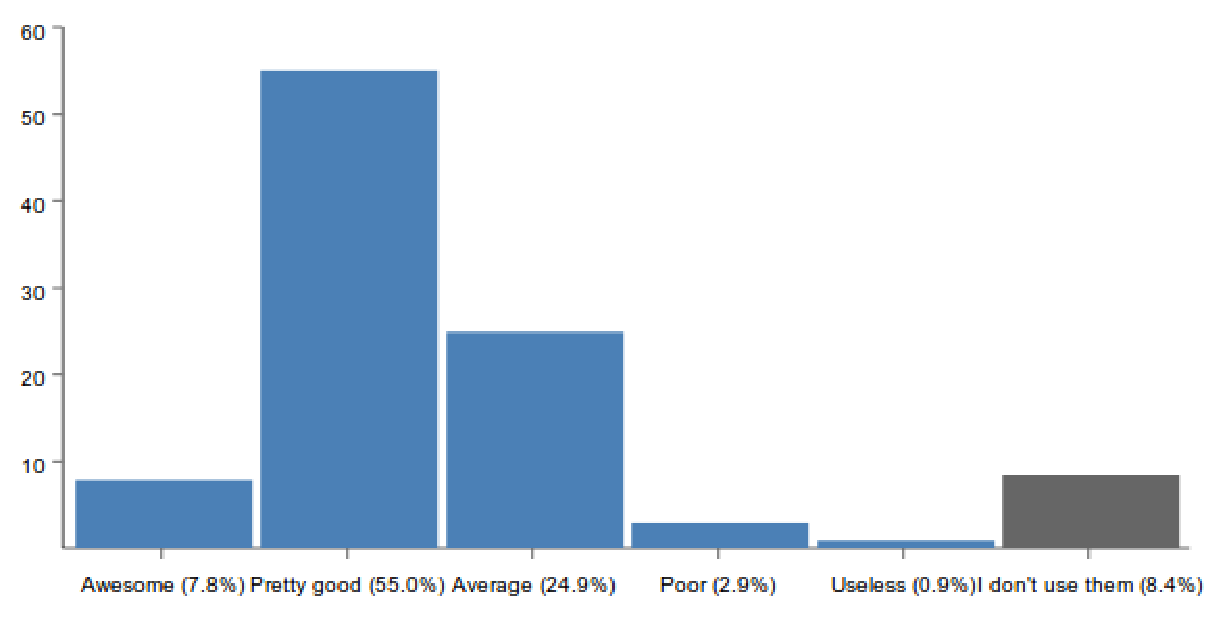
\includegraphics[width=\textwidth]{../images/enquete/think-of-recommendations}
          \label{fig:recommendations}
          \end{center}
        \end{figure}

      \paragraph{}Qua kwaliteit van de aanbevelingen, te zien in figuur \ref{fig:recommendations}, zijn de meeste mensen tevreden. 87.7\% vind de aanbevelingen gemiddeld of bovengemiddeld, en 62.8 vind ze bovengemiddeld goed. een klein percentage van acht-en-een-half procent gebruikt de aanbevelingen in totaal niet. Zoals eerder genoemd zouden we de aanbevelingen exclusiever kunnen laten lijken door er minder tegelijk te laten zien, of per categorie éen aanbeveling te laten zien.

      Uit figuur \ref{fig:advertisements} blijkt dat het overgrote deel van de respondenten de advertenties niet merken of niet als vervelend ervaren. Deze wetenschap kan een rol spelen bij het plaatsen van advertenties op andere pagina's. Wanneer mensen de advertenties op dit moment niet merken, kunnen deze op een zichtbaardere plaats worden neergezet, wat tot een hogere click-through rate zou moeten leiden.

        \begin{figure}
          \begin{center}
          \caption{Wat vinden respondenten van de advertenties}
            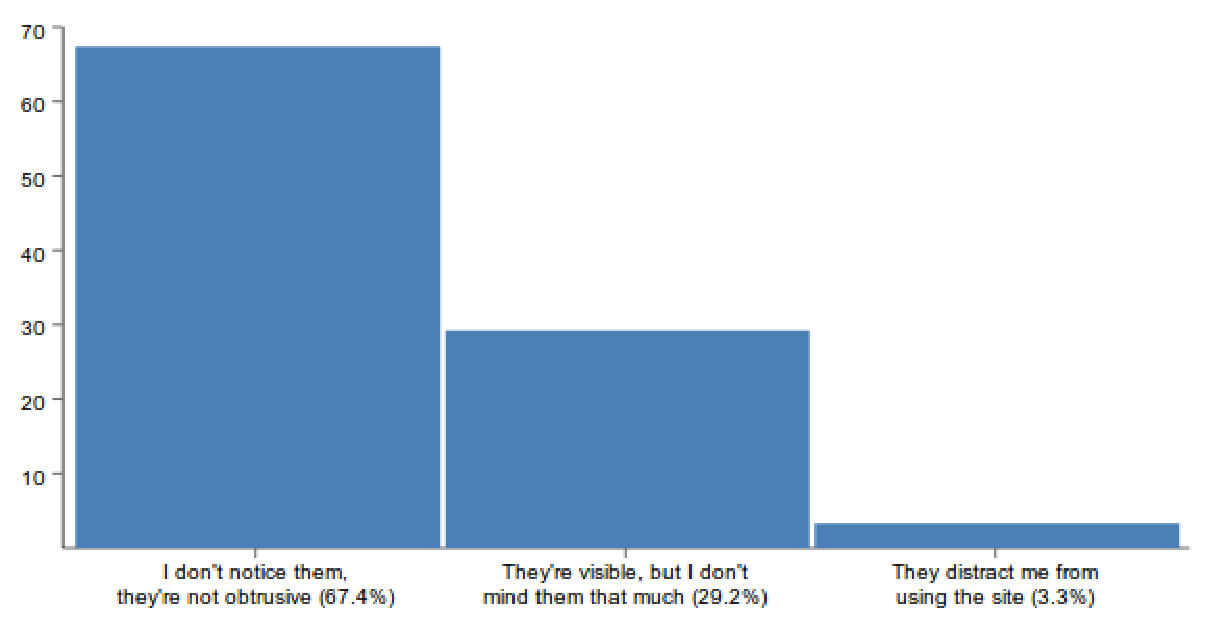
\includegraphics[width=\textwidth]{../images/enquete/advertisements}
          \label{fig:advertisements}
          \end{center}
        \end{figure}



  \chapter{Persona's}
    \label{personasappendix}
De onderstaande persona's zijn gebaseerd op de interne doelgroepanalyse van Wakoopa en de gegevens uit de uitgevoerde Enqu\^ete.

\section{Tom Daaler}
  \begin{wrapfigure}{l}{40mm}
      
\includegraphics[height=40mm]{../images/personas/tom}
  \end{wrapfigure}
Tom is 17 jaar en zit in zijn laatste jaar havo. Hij werkt als vakkenvuller bij de AH en spendeert de meeste de meeste van zijn vrije tijd achter de pc waar hij games speelt of zijn pc aan het tweaken is. Het geld wat hij bij de AH verdient gaat voornamelijk op aan games en hardware. Hij is nieuwsgierig en probeert daarom vaak nieuwe programma's. Wanneer hij een nieuw programma ontdekt is hij vaak een van de eerste onder zijn vrienden, en is trots als hij zijn bevindingen kan delen en aan anderen uit kan leggen hoe een nieuw programma werkt.

In het MBTI model zoals gebruikt in \cite{Klompsma} is Tom een competetieve bezoeker.

\section{Andreas Nilsson}
  \begin{wrapfigure}{l}{40mm}
      
\includegraphics[height=40mm]{../images/personas/andreas}
  \end{wrapfigure}
Andreas is 28 jaar en heeft een baan bij een IT-bedrijf als programmeur. Buiten zijn werk probeert hij de computer te ontwijken, hoewel hij 's avonds vaak nog even op youtube of hyves zit. Hij wil graag zo efficient mogelijk werken en ergert zich snel aan programma's. Daarintegen wilt hij ook niet teveel tijd besteden aan het vinden en uitzoeken van nieuwe programma's. Het is voor hem belangrijk dat hij zo goed mogelijk zijn werk kan doen en daarbij niet teveel aan andere dingen hoeft te denken. Andreas moet van zijn bedrijf bijhouden waar zijn tijd aan opgaat, iets waar hij eigelijk niet op zit te wachten.

In het MBTI model zoals gebruikt in \cite{Klompsma} is Andreas een competetieve bezoeker.

\section{Johan Broers}
  \begin{wrapfigure}{l}{40mm}
      
\includegraphics[height=40mm]{../images/personas/johan}
  \end{wrapfigure}
Johan is 32 en de maker van TimeSink, een klein programma om je tijd te managen. Hiervan heeft hij een gratis versie en een betaalde versie met meer opties. Naast dit programma werkt hij zelf als freelancer voor verschillende softwarebedrijven, maar het liefst zou hij genoeg verdienen om eigen baas te kunnen worden. hij komt graag in contact met gebruikers van zijn programma en is zeer geinteresseerd in wat ze van zijn programma vinden. Hij kijkt vaak naar zijn downloadstatistieken, maar blijft benieuwd naar hoeveel mensen zijn programma nou echt gebruiken.

In het MBTI model zoals gebruikt in \cite{Klompsma} is Johan een humanistische bezoeker.

\section{Mariette Klompman}
  \begin{wrapfigure}{l}{40mm}
      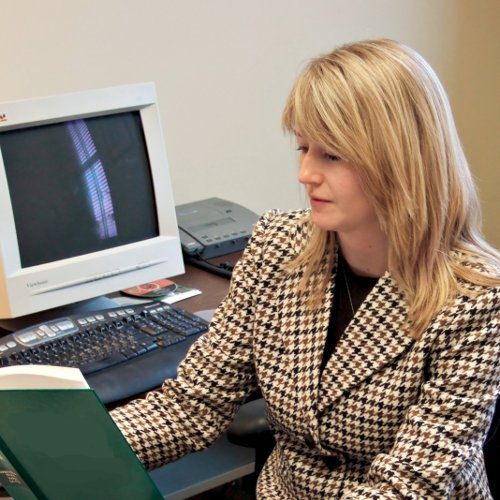
\includegraphics[height=40mm]{../images/personas/mariette}
  \end{wrapfigure}
Mariette is een administratief medewerker voor een scholengemeenschap en moeder van 2 kinderen van 8 en 5. Voor haar werk zit ze veel in microsoft office, maar thuis doet ze eigelijk niks met de computer. In haar vrije tijd loopt ze hard en schildert ze. Ze is niet heel vaardig met computer, ondanks dat ze voor haar werk een cursus office en internet heeft gevolgd. Soms loopt ze vast met word, en vraagt dan haar collega om hulp. Op dagen dat haar collega er niet is, probeerd ze via google toch het antwoord te vinden, maar vaak vind ze niet wat ze zoekt, of ze snapt de gebruikte termen niet helemaal. Als ze het niet snel kan vinden schrijft ze het om op later aan haar collega te vragen en gaat dan ergens anders mee verder.

In het MBTI model zoals gebruikt in \cite{Klompsma} is Mariette een spontane bezoeker.



  \chapter{Lab tests analyses}
    \label{labtestsappendix}

\section{Claudia Engelsman}
\textbf{19 jaar, past bij persona van Mariette.}

\subsection{Opdracht 1}
  Ziet het zoekveld niet en scrollt initieel niet ver genoeg terug naar boven om het te zien. Klikt een aantal keer direct naast het zoekveld op andere opties en komt uiteindelijk op een toplijst, waaruit ze een programma kiest. Eenmaal op de pagina is het schrijven van een review geen probleem

\subsection{Opdracht 2}
  Zoekt naar `websites' in het zoekveld, maar de site reageert erg traag, zo erg dat ze zich afvraagt op het werkt. eenmaal op de zoekpagina klikt ze vrij snel op adobe dreamweaver, totdat ze zich realiseert dat dat geen website is. Ze gaat weg van de zoekpagina en is verward over de verdeling tussen websites en programma's. Via het eigen profiel klikt ze op twitter om dit vervolgens in haar browser toe te voegen als favorite. Hierop heb ik de benaming aangepast

\subsection{Opdracht 3}
  Ze klikt doelgericht naar het eigen profiel en bekijk de pagina. Vervolgens klikt ze bij de grafiek op "today".

\subsection{Opdracht 4}
 Ze klikt direct op people maar kan het daar niet vinden, ze klikt op het dropdown menu van you en op "find en invite people". Ze staat op het punt om het op te geven en klikt door naar het dashboard. Ze zegt dat er wel software recommendations zijn, maar niet gebruikers. Ze scrollt verder naar beneden en meld "oh, ik wist niet dat je ook buren kon hebben", maar ziet dit niet als zijnde `mensen die op je lijken', dit merkt ze ook op. Ze klikt door naar software recommendations, waar "neighbours" wordt uitgelegd. Op het profiel heeft ze geen probleem de persoon als contact toe te voegen.

\subsection{Opdracht 5}
 Ze zoekt teams bij you en bij dashboard, vervolgens bij software en dan naar categorien, die ze als teams ziet. ze klikt door naar een programme en merkt dan op dat het `zeker geen team is'. Ze zoekt in de zoekbalk naar `team', kijkt moeilijk en klikt dan op de teams lijst. Ze zoekt naar twee applicaties, rollercoaster tycoon en spore, waarbij de laatste een team heeft. Eenmaal op de teampagina klikt ze vrij snel op `join this team.'

 \subsection{Algemeen}
  Over het algemeen liggen voor Claudia de meeste problemen in de terminologie en de navigatie. Wanneer ze eenmaal op een pagina zit, vind ze vaak snel waar ze naar zoekt.

\section{Mark van der Ham}
\textbf{20 jaar, past bij persona van Tom.}

\subsection{Opdracht 1}
Klik gelijk door naar Reviews, en zoekt daarna naar Itunes, scrolled vrij lang door de lijst. In de nabespreking gaf hij aan dat het te druk was en dat de verschillende programma's die op itunes leken hem verwarden. Na een aantal keer scrollen klikt hij op de eerste hit. Zodra hij op de itunes pagina zit vind hij het reviewformulier snel

\subsection{Opdracht 2}
Zoek naar een site die niet op wakoopa staat, met de volledige url. Na een opmerking over wat voor sites het moet gaan, zoekt hij op hyves en vind snel de favorite-knop. Vult een erg lange tekst in ondanks het kleine invoerveld.

\subsection{Opdracht 3}
Klik vrij zeker op you, scrollt naar Usage, klikt op Today, maar denkt daarna dat het 'usage in the last hour' het gebruik vandaag is en laat het verder daarbij.

\subsection{Opdracht 4}
Bekijkt vrij lang de persoonlijke profielpagina. Zoekt dan op "developer" en bekijkt het profiel van een van de hits. Gaat dan terug naar het eigen profiel, naar usage and contacts. Zegt dat hij iets van aanbevelingen zoekt maar dat niet kan vinden. Klikt door naar find and invite en ziet dan een link naar recommendations. Leest het tekstje en zegt dat hij het gevonden heeft.

Op het profiel zegt hij dat het al een contact is en wijs op een lege plek naar de block button. Scrollt omlaag en omhoog en ziet dan de "add link".

\subsection{Opdracht 5}
klikt door naar teams, en zoekt naar ultrabeat, waar geen team voor wordt gevonden. Zoekt vervolgens naar 'call of duty' via het zoekveld, die automatisch op software in plaats van developers zoekt. Klikt door naar software, en doet dit een aantal keer. Klik door naar users en merkt op dat het geen team is. Klikt terug naar de teams pagina en klikt op gamers. Op de teampagina klikt hij direct op "join this team".

\subsection{Algemeen}
Mark heeft de dashboard, je eigen startpagina, helemaal niet gezien. Dit had wellicht geholpen bij het vinden van in ieder geval de aanbevelingen. Een grote fout was dat bij het zoeken niet onthouden werd naar wat voor soort dingen gezocht werd, en dat dit er niet duidelijk bovenstond. In opdracht 5 lukte het Mark daarom niet goed een team te vinden.

\section{Mark Dekkers Los}
\textbf{22 jaar, past bij persona van Andreas.}

\subsection{Opdracht 1}
Klik op software en gaat dan naar categories. Vind daar de zoekbalk. Zoekt op quicktime en klikt op het eerste resultaat. Klikt daar gelijk door naar Reviews, en dan in de rechterbovenhoek op "Write one!". Schrijft een review, kijkt even naar de andere reviews en voegt dan ook een rating toe.

\subsection{Opdracht 2}
Klikt op het logo om naar het dashboard, klikt de verschillende menu's aan, en zoekt vervolgens op "website". Zoekt door de resultaten en vindt Facebook. Scrollt over de hele pagina en weer terug, en klikt dan op favorite.

\subsection{Opdracht 3}
Klikt op het profiel en kijkt naar recently used, type of usage and ziet dan "today" bij de grafiek. Klikt op today.

\subsection{Opdracht 4}
Klikt op people, kijkt daar even en wilt gaan zoeken, maar kan niet op een term geven. Vraagt op welke manier ze op elkaar moeten lijken, met het antwoord dat Wakoopa dat aangeeft. Klikt bij people op reviews, en twijfelt vervolgens in het dropdown menu tussen find and invite en recommendations. Klikt op recommendations, vind de neighbours en klikt direct op het toevoegen icoontje.

\subsection{Opdracht 5}
Gaat naar teams, zoekt op "call of duty", merkt op dat het team spaans is en klikt vrij direct op join this team.

\subsection{Algemeen}
Er zijn geen algemeen opvallende dingen aan deze labtest.

\section{Jorn van Schaik}
\textbf{20 jaar, past bij persona van Tom.}

\subsection{Opdracht 1}
Bekijkt het dashboard en klikt op verschillende plekken. Gaat naar het zoekveld en typt dan een zin in, maar zoekt niet. Klikt vervolgens op quicktime player. Geeft later aan dat hij het logischer vondt als je eerst aangaf een review te willen schrijven, en daarna pas waarover in plaats van andersom. Op de softwarepagina vind hij erg snel de review-mogelijkheid.

\subsection{Opdracht 2}
gaat naar het zoekveld en zoekt op een volledige site (url) en vind dan niks. Gaat terug naar de dashboard en klikt dan op "Find and invite". Bekijkt de dropdowns en kijkt verder rond. Vraagt of het op Wakoopa moet. Klikt vervolgens zonder iets te typen op de zoekknop, waardoor er naar "search for..." wordt gezocht. Klikt dan op Google search en vind op de pagina heel snel de favorite knop

\subsection{Opdracht 3}
Klikt direct op de dropdown bij `you' en klikt dan op settings en gaat naar favorites. Bekijkt nogmaals de dropdowns, scrollt naar beneden en klikt op help. Scrollt heen en weer en klikt uiteindelijk op You. Ziet de grafiek, maar selecteert de `top used applications' in plaats van category usage.

\subsection{Opdracht 4}
Klikt direct in de dropdown bij `you' op recommendations, leest het stuk over neighbours, klikt door naar de gebruiker en klikt daar snel op `add as contact'

\subsection{Opdracht 5}
Bekijkt alle dropdowns nogmaals en klikt dan door op `teams'. Bekijkt de pagina maar zoekt niet. Klikt uiteindelijk op een groep en klikt vervolgens direct op `join this team'

\subsection{Algemeen}
Jorn klikte veel en vond daardoor veel functies al voordat hij ze nodig had. Hierdoor kreeg hij snel feeling voor hoe de site in elkaar zat. Opvallend is dat, hoewel hij de zoekfunctie wel heeft gebruikt, en iets in het zoekveld getypt, heeft hij niet bewust naar iets gezocht. Na afloop gaf hij aan dat hij dit gemakkelijker vond.


  \chapter{Interviews}
\label{interviewappendix}
Er zijn drie usability experts ge\"interviewd over hun ervaringen met learning networks, usability en hun visie daarop. Voor dit interview is een losse structuur aangehouden, met de volgende vragen als leidraad:

\begin{itemize}
  \item Welke learning networks gebruik je zelf?
  \item Welke learning networks zijn goede voorbeelden van usability en welke minder?

  \item Welke struikelblokken kom je tegen op learning networks's tijdens onderzoeken
  \item Hoe ga je daar mee om tijdens het beoordelen of ontwerpen van een learning networks, wat zijn oplossingen?

  \item Zijn er recente stijl/designontwikkelijken, op usability gebied (zoals bijvoorbeeld google suggest) die je goed vind
  \item En slecht?

  \item Welke onderzoeksmethodieken zijn jouw favoriet? Als je veel budget hebt, en als je weinig budget hebt?
  \item Is er een methode die je verrast heeft toen je hem voor het eerst gebruikte?

  \item Welke methodieken vind jij handig voor learning networks?
  \item Welke vind je minder handig?

  \item Waar zie jij het vakgebied in de toekomst heengaan, wat zijn opkomende technieken volgens jou?
\end{itemize}

Er is gekozen voor deze losse structuur omdat usability een heel breed gebied is. Iedere expert heeft een specialisatie en door de vrijheid te laten kan de expert zijn expertise toepassen op de gestelde vragen.

\section{Bas Bakker}
Bas Bakker is een zelfstandig ondernemer die is afgestudeerd op het ontwerpen en bouwen van een learning network, `goedkado.nl'. Dit is een website waarop mensen kadotips voor vrienden kunnen krijgen aan de hand van integratie met bijvoorbeeld hyves. Bas maakt geregeld expert reviews voor bestaande websites.

\paragraph{}
\textbf{Kilian:} Welke learning networks ben je zelf op actief?

\textbf{Bas:} Ik heb net geleerd dat hyves geen learning network is. Ik gebruik linkedin, flickr, en youtube gebruik ik wel eens, maar wie doet dat nou niet? Twitter gebruik ik ook, maar ik geloof niet dat dat er onder valt. Ning, ik weet niet of dat er onder valt, dat ligt eraan welk ning netwerk natuurlijk. Dit waren zowiezo wel de hoofddingen die ik gebruik.

\textbf{Kilian:} Heb je misschien voorbeelden van hoe Ning ingedeeld kan worden?

\textbf{Bas:} Er zijn twee verschillende voorbeelden. De een is vooral netwerken en de andere is inderdaad meer community waar je ook leert. Wat je veel ziet is dat nings worden opgericht op basis van een offline netwerk. mensen die een community maken om in contact met elkaar te blijven. Opencoffee leiden is daar een voorbeeld van, maar daar gebeurt niet zoveel. Een ander voorbeeld is bijvoorbeeld die van de zaanstreek, daar laten ze zien hoe mooi de zaanstreek is, plaatsen er foto's op en er zijn discussies. De dingen waar ik Ning het meest voor gebruik beginnen offline en gaan dan ook online.

\textbf{Kilian:} Als je kijkt naar ning, of learning networks in het algemeen, zijn er dan gelijk al dingen die je zelf anders zou doen op het gebied van usability?

\textbf{Bas:} Daar moet ik even over denken. Ik vind het concept van ning best slim, zakelijk, en voor niks kan je een netwerk opzetten. Qua usability laat het te wensen over. Het gaat nu vooral over "nu en wat er nog komen gaat". Een gebeurtenis verdwijnt uiteindelijk en dan moet je gaan graven om dat terug te vinden. Dus om een community in te gaan is vrij moeilijk. Dat zou beter kunnen. En de algemene usability...Je moet het een keertje doen, en dan ga je het pas begrijpen. Dat zie je bij heel veel communities, Je komt er, en dan is er geen doel voor jou. Het is vrijheid blijheid, en je kan alle kanten op. Mensen verliezen zich daar in. Dat zie je bij twitter. Mensen zitten daar zonder dat ze weten wat ze aan het doen zijn. Daarnaast draagt het ook niet altijd bij aan het netwerk.

Een voorbeeld daarvan is bij meetup, een website om bij conferenties te zeggen dat je ook komt, de grootste groep daar is werkeloze huismoeders die thuis zitten en met elkaar in contact willen komen. Ieder sociaal netwerk zorgt ervoor dat mensen zelf hun doel kunnen bepalen. Als ze dat hebben gevonden gaan mensen er wel heen, alleen wanneer ze beginnen denken veel mensen "wat moet ik hier mee?". Bij ning zie je dat als je er komt, dan weet je niet wat er in het verleden is gebeurd, en dan weet je niet wat je daar mee moet. Wat je ziet is dat mensen zich aanmelden en ze worden actief, of ze komen nooit meer terug.

\textbf{Kilian:} Ning is dus goed als ondersteunend van een offline community, dus wat je meer moet hebben is dat mensen in het verleden dingen hebben gedaan en daar over verder praten en dingen mee kunnen doen in plaats van enkel in de toekomst kijken.

\textbf{Bas:} Op zich zijn er ook wel genoeg netwerken op Ning die enkel online zijn. Dan nog is het heel moeilijk om er in te graven. Het is een forum, en als je eenmaal 100 discussies verder bent weet je niet wat er heeft gespeeld. Als je er al een tijdje bent is dat geen probleem, maar als nieuwe gebruiker moet je eerst een hoop onderzoek doen naar wat er al is gebeurd. Als je dat niet doet wordt je direct raar aangekijken. Ning is eigelijk net een stap verder dan een forum want het kan iets meer, maar het is slechts éen stapje verder. Het mist het directe doel.

\textbf{Kilian:} Is dat iets wat jij als je zelf iets zou bouwen, wat jij zou doen? Als je op de site komt dat je gelijk aangeeft "dit is het doel"?

\textbf{Bas:} Dat ligt eraan wat het doel is van wat je bouwt. Bij een klant die een sociaal netwerk wilt maken zoals Hyves, dan zou ik dat niet doen. Maar als je een netwerk rondom initiatieven maakt, dan moet je wel neerzetten wat het initiatief is. Bijvoorbeeld bij Flickr is het heel duidelijk dat het om foto's gaat. Als het echt om éen ding gaat, als learning network, dan moet je dat wel neerzetten ja. Bij hyves kan je het niet in drie zinnen neerzetten omdat er zoveel manieren zijn.

\textbf{Kilian:} Hoe zou dat doel gepresenteerd moeten worden? Als die drie regels uitleg, of een complete tutorial?

\textbf{Bas:} Ja, ik zou het allebij doen. Het moet zowiezo in éen oogopslag duidelijk zijn. Voor de "luie bezoeker" moet het gelijk duidelijk zijn, en als iemand meer informatie wilt, dan moet het ook beschikbaar zijn, dan moet er ook die tutorial zijn. Maar als die eerste doelen weg zijn dan moeten mensen dus een tutorial doorlopen om te weten waar het over gaat. Bijvoorbeeld Google wave, dat kwam uit en toen moest je een film van een uur kijken. Ik heb het niet gedaan. Toen ging ik google wave kijken en ik snapte er niks van. Nu heb ik er een beetje mee gespeeld en is het wel leuk, maar dat is een beetje dat vrijheid blijheid. Er zit geen doel achter, en dan moet je veel uitleggen. Maar ik denk op het moment dat je zegt "dit zijn de doelen" dan is dat helder, en daarna met meer informatie als mensen dat willen.

\textbf{Kilian:} Een recente trend om een learning network in een video uit te leggen. Wat vind jij daar van?

\textbf{Bas:} Als je kijkt hoe dat werkt met leren, dan leer je eerst iets, dat commit je en dan ga je het doen, en dan ga je weer leren, commiten, doen en zo voorts. Dus je zal het eerst moeten leren. Qua design kan je dingen zo duidelijk mogelijk maken. Bijvoorbeeld met een duidelijke call to action. Ook hier is beide weer beter. Een video maken kost gewoon tijd, maar het is wel duidelijk. Mensen focussen zich op een video, en op een site niet. Als je een video aanzet, zijn mensen daarop gefocussed terwijl ze op een site overal kijken. Alleen mensen verplichten is weer geen goed idee. Je moet een balans vinden tussen een intuitief design, en daarnaast een video om het uit te leggen. Je hebt altijd de helft blijft en de helft gaat wel weg.

\textbf{Kilian:} Dus zoveel mogelijk verschillende manieren werkt volgens jou het best?

\textbf{Bas:} nouja, niet zoveel mogelijk, maar wel meerdere.

\textbf{Kilian:} De site van jouw afstudeerproject, goedkado, is ook een soort learning network, ben je daar ook problemen tegen gekomen qua usability?

\textbf{Bas:} Ja, daar moet ik even over denken. Een van de dingen was dat de navigatie aan de linkerkant stond en totaal over het hoofd werd gezien. Ik had een aanname gedaan door dit over te nemen van bol.com en amazon die dat ook allebei doen. Mensen zagen dat niet. Dat was gemakkelijk op te lossen door de navigatie bovenaan overdwars te zetten. Een ander punt is dat de labels van navigatie en de structuur van de site. Je doet aannames over wat je doet en koppelt daar namen aan. Bijvoorbeeld 'kadotips'. We geven je kadotips voor vrienden, maar het is heel onduidelijk wat dat betekend omdat mensen daar niet bekend mee zijn. Ze weten niet voor wie, en wat daar achter zit. Ze wilden zoeken bij kado's, en niet bij kadotips. Jouw gedachten en aannames sluiten soms niet aan bij wat de meeste gebruikers vinden. Er zit ook een deel uitleggen bij, mensen wisten niet waarvoor die kadotips dan waren, en hoe ze gemaakt werden. Ze willen weten hoe het werkt. Die beschrijvingen zou er ook bij moeten.

\textbf{Kilian:} Het gaat dus erg om de uitleg, en mensen willen het begrijpen en daar moet je in voorzien.

\textbf{Bas:} Ja dat klopt. Je probeert een probleem op te lossen, maar in de loop van de jaren zijn mensen daar wantrouwig naar geworden. Ze geloven niet dat dat vanzelf gaat, dus ze willen weten hoe het probleem wordt opgelost. Niet technisch natuurlijk, maar gewoon in normale taal, dat inzicht.

\textbf{Kilian:} Je zegt dus eigelijk dat in plaats van aangeven dat er een probleem is, wat vaak gebeurt, dat je ook moet uitleggen hoe je dat op kan lossen?

\textbf{Bas:} Dus eigelijk, dat je het probleem oplost is niet genoeg, je moet het oplossen. Het heeft vooral met vertrouwen te maken. Dit zie je ook bij de aanbevelingen op bol.com en amazon. Ik bekijk dat altijd, maar het is wel interessant om te weten hoe die gemaakt worden. Misschien past dat wel helemaal niet bij mij. Ik kan zelf wel een selectie van interessante aanbevelingen maken, maar het is ook interessant om te weten wat voor soort mensen dan precies die aanbevelingen kochten. Met dat kan ik gelijk een selectie maken van wat wel en niet interessant is voor mij. Het komt dus terug op dat je het vertrouwen moet krijgen. Je moet kijken naar de twee soort personen. Je hebt mensen die snel keuzes maken, en mensen die meer de diepte in willen en snel kunnen schakelen.

\textbf{Kilian:} Dat klopt ook wel met een artikel wat ik voor mij scriptie hebt gebruikt over persona's, daar zijn vier typen mensen. Er zijn mensen die snel gebaseerd op feiten of snel gebaseerd op emotie en mensen die sloom gebaseerd op feiten of snel gebaseerd op emotie beslissen. Dat klopt ook wel met jouw indeling volgens mij.

\textbf{Bas:} Ik denk inderdaad dat het zo werkt. Iedereen is natuurlijk uniek in zijn denken. Iedereen heeft zijn eigen perspectief. Maar op het moment dat jij een van de twee groepen niet faciliteerd, dan verlies je ze. Specialisten die willen de feiten en weten hoe ze dat kunnen controleren, en de generalisten willen juist snel kunnen zien waar het over gaat. Daar moet je een balans tussen vinden.

\textbf{Kilian:} Op Wakoopa staan ook recommendations, en daar is ook veel behoefte aan uitleg. Volgens mij komt dat omdat er vooral de specialisten op wakoopa zitten, en die willen volgens mij vaak weten hoe het precies zit. Dat is lastig omdat het via een wiskundige formule werkt die software en gebruik aan elkaar koppelt. Je krijgt dus een aanbeveling omdat je iets anders al gebruikt.

\textbf{Bas:} Volgens mij komt dat ook een beetje omdat je op wakoopa niet direct op zoek bent naar iets nieuws. Bij bol.com ben je echt op zoek naar een boek. Bij wakoopa heb je al je programma's, je zit in een bepaalde comfort zone. Je weet bijvoorbeeld hoe photoshop 6 werkt, en een aanbeveling zou dan photoshop 7 kunnen zijn. Je geeft dan aan dat ze uit hun comfort zone moeten, en even tijd steken in het leren van iets nieuws, en veel mensen hebben dan zoiet van "wacht even". Een van de gouden regels van een veranderingsproces is dat mensen pas veranderen als ze daar zelf inbreng in hebben. Software is een keuze, maar je kan ook denken "dit is de aanbeveling en dit is waarom", en dan kan je er bij bedenken dat ze iets er zelf ook over kunnen beslissen. Dat proces is dan veel gemakkelijker.

\textbf{Kilian:} Eigelijk zou je dus een aanbevelingstraject zou moeten hebben. Nu geven we een lijst, maar misschien kan je laten zien wat andere mensen beter vinden aan dat nieuwe programma.

\textbf{Bas:} Stel dat je photoshop gebruikt, en als aanbeveling illustrator hebt. Dat je dan aan kan geven dat het handig is voor logodesign. En dat je dan kan zeggen "ik maak geen logo's, ik maak websites" en dat je niks met vectoren doet. Dat er dan uitkomt dat je illustrator niet moet gaan gebruiken, of juist dat je wel logo's maakt en dat illustrator dan wel een goede tips is. Je moet aangeven wat het doel is voor een gebruiker.

\textbf{Kilian:} in de afgelopen paar jaar zijn er usability methodes bijgekomen, zoals video's die veel effectiever blijken, of google suggest die je suggesties geven. Zijn er dingen die er voor jou uitspringen op dat gebied?

\textbf{Bas:} Nou, wat ik vaak tegenkom en gebruik zijn wel de video's, dat geeft gelijk een beeld. Google suggest gaat volgens mij nog niet ver genoeg, ik wil graag dat als ik fiets zoek dat er dan ook "probeer eens rijwiel" bij komt. Ik ben niet heel veel bezig met dat soort dingen. Het is meer op gevoel, dat het hele plaatje klopt.

\textbf{Kilian:} Hoe onderzoek je zelf sites op usability? Waar let je dan precies op?

\textbf{Bas:} Waar ik op let is pure acties. Ik maak vooral commerciele sites. Op elke pagina moet er een actie voor een gebruiker zijn. Een voorbeeld wat ik laatst in een website heb gedaan is het toevoegen van een offerteformulier, naast een contactformulier. Je merkt dat mensen dat toch gaan gebruiken en dat er een week later al offerteaanvragen binnen komen. Volgens mij is dat het belangrijkste, dat er altijd een actie voor de gebruiker is.

\textbf{Kilian:} Welke methodieken gebruik je zelf voor usability onderzoek?

\textbf{Bas:} Ik doe eigelijk enkel expert reviews en statistiekanalyse. Uiteindelijk moet een klant er voor betalen en gebruikersonderzoek neemt veel tijd in beslag. Ik wil het wel doen, maar het geld daarvoor is er niet bij de klanten die ik nu heb. Ik kijk naar de paden die mensen op een site doorlopen, maar dat heeft natuurlijk beperkingen. Je doet aannames op basis van de gegevens die je hebt. Je weet bijvoorbeeld niet of mensen boven of onderaan op een knop klikken, enkel naar welke pagina's te gaan. Ook weet je vaak niet met wat voor doel ze op een site komen, wat voor soort mensen het zijn.

\textbf{Kilian:} Waar zie jij het vakgebied in de toekomst heen gaan?

\textbf{Bas:} Er zijn nu heel veel verschillende online tools en dingen die bepaalde dingen doen, zoals bijvoorbeeld Silverback. Google die doet ook steeds meer, analytics heeft nu bijvoorbeeld een api waardoor je veel meer kan analyseren, hoewel je je wel af kan vragen of sommige van die dingen wel geanalyseerd moeten worden. Volgens mij komen er in de toekomst veel meer tools die al dat soort dingen samen doen, als groot omvattend iets zegmaar. Door met meer data verbanden te leggen kan je weer betere aannames maken. Het is nu heel erg versplinterd, en ik denk dat dat langzaam samen zal komen.

\section{Ruben Timmerman}
Ruben Timmerman Is eigenaar van Usearchy en doet veel expert reviews en gebruikersonderzoek voor andere bedrijven. Zijn meest recente project is het aan de wieg staan van het Hyves herontwerp en het begeleiden van dat proces.

\paragraph{}
\textbf{Kilian:} Welke learning networks gebruik je zelf?

\textbf{Ruben:} Flickr en Wakoopa, linkedin, maar dat is misschien meer sociaal. Waarschijnlijk nog veel meer, maar dan zou ik even moeten denken. Heb je nog suggesties?

\textbf{Kilian:} Bijvoorbeeld iets als linksharing

\textbf{Ruben:} Doe ik weinig aan, af en toe slideshare. Delicious gebruik ik eigelijk bijna niet meer. Ik gebruik google docs, maar ik weet niet of dat een learning network is. Je shared je docs, maar het is natuurlijk niet open. Je kiest je eigen network. Wij gebruiken hier enkel google docs, maar het is wat minder vrij

\textbf{Kilian:} Welke learning networks hebben hun usability goed op orde, en welke niet?

\textbf{Ruben:} Eigelijk allemaal wel. Ik ben een late adopter, dus de networks die ik gebruik, gebruik ik omdat ze al succesvol zijn. Ik heb nu google wave bijvoorbeeld nog niet gebruikt omdat ik het nut er nog niet van in zie. Dan ga ik het pas gebruiken. Er zijn niet echt networks waar ik ontevreden over ben. Van slideshare kan ik soms wel zeggen dat het niet helemaal geweldig is. Van Flickr heb ik soms echt wel van "wow, wat hebben ze dat slim of handig gedaan". Maar slideshare kan ik prima gebruiken, dus ik zie daar niet echt problemen mee.

\textbf{Kilian:} Heb je al naar google wave gekeken?

\textbf{Ruben:} Nog niet echt. Wat ik hoop dat gaat gebeuren is dat andere bedrijven het googlewave protocol gaan gebruiken voor hun aplicaties, en dat die usability er dan dus al ingebakken zit.

\textbf{Kilian:} Jij doet ook wel eens expert reviews op learning networks. Wat zijn daar de struikelblokken?

\textbf{Ruben:} Ik kijk dan toch stiekem even naar hyves, en dan de delen die onder een learning network kunnen vallen. De herbruikbaarheid van objecten binnen verschillende concepten is een enorm probleem daar. Wat we bijvoorbeeld hadden was het object foto, daar moet je vanalles mee moeten kunnen doen. Dat kan in verschillende contexten, zoals bijvoorbeeld in een bericht, of in een album. Je hebt dan hetzelfde concept ("het bewerken van een foto") in een andere context. We hebben alle objecten en contexten uitgeschreven, dat zijn honderden pagina's waarbij we voor alle objecten opgeschreven waar en op welke manier ze gebruikt worden. Het grootste probleem of uitdaging is volgens mij zorgen dat dat over de hele site klopt.

\textbf{Kilian:} Bij wakoopa hebben we heel erg dat het benoemen van delen of functies. Hoe jij er over denkt is heel anders dan hoe anderen daar over denken.

\textbf{Ruben:} Bij hyves hebben we dat ook altijd gehad. Hoe zij dat oplosten was door middel van een courtesylinkje, en elke keer was dat zo. Gebruikers verwachten dingen op andere plekken, en op een gegeven moment ben je overal linkjes aan het plaatsen. Dat is een probleem

\textbf{Kilian:} Overal linkjes is natuurlijk ook niet optimaal, hoe ga je daar mee om?

\textbf{Ruben:} Waar je dan op komt is dat je je gebruikers eigelijk wilt educaten. Je wilt ze iets gaan leren. Je moet iets bedenken waarbij je de link tussen objecten, dus niet een echte link, maar de link in iemands hoofd, duidelijker moet gaan maken. Door gebruik van hetzelfde icoon, of eenduidig taalgebruik of iets dergelijks. Waar we bij hyves heel vaak op kwamen was dat een aantal verschillende elementen die in de loop van de jaren zijn gemaakt eigelijk heel erg op elkaar lijken. Wat we dan moeten doen is ze groeperen of op elkaar te laten lijken zodat de band tussen de elementen duidelijk is. Je wilt dat omgooien en hetzelfde maken, maar dat moet je dan stapje voor stapje doen. Door dat stukje bij beetje online te zetten zorg je dat gebruikers langzaam leren wat de relatie tussen objecten is. Dat is moeilijk want je maakt toch een beslissing om alles om te gooien.

\textbf{Kilian:} Maak jij veel gebruik van design patterns, kijkend naar het samenvoegen van die concepten?

\textbf{Ruben:} Ja, naast dat je objecten in meerdere contexten kan hebben, zoals een foto editten in een bericht of in een fotoalbum, krijg je ook dat je een video kan editten, en een krabbel kan editten. En daar wil je ook regels voor. Bij hyves is het voornamelijkste wat we daar gedaan hebben is het tekstveld. de Rich text editors verschilde heel erg, en daar hebben we een ding van gemaakt. Een van de eerste dingen die ik daar heb geroepen is dat ze patterns moesten gaan maken. De patterns en de context zijn dus eigelijk de twee dimensies.

\textbf{Kilian:} Zijn er recente stijlontwikkelingen die jou opvallen op het gebied van usability? zoals google suggest, of de google wave scrollbars, of iets heel anders als een video op de homepagina.

\textbf{Ruben:} Moeilijk om daar snel antwoord op te geven. De truuk is om het wiel niet opnieuw uit te vinden. Als jij een learning network hebt, begin met de succesvolste en bouw die naar. Met Eduhub heb ik hetzelfde gedaan, dat is een vergelijkingssite voor opleidingen, en daar heb ik booking.com en funda voor nagebouwd. Pas daarna ben ik zelf dingen aan gaan passen. Maar om trends te noemen. Je ziet ze op allerlei niveau's. In vergelijkingsland is het bijvoorbeeld normaal om meerdere resultaten te vergelijken door middel van vinkjes naast de resultaten. In de e-commerce zie je ze nog sterker, zoals bijvoorbeeld direct onder de bestelbutton een goed-gevoel zinnetje te zetten. Iets als "het is op vooraad, en u heeft het altijd binnen een dag in huis". Dat soort patronen zie je heel erg terug. Je ziet ook dat de grote namen elkaar nadoen of tot dezelfde oplossing komen. Als de interaction designers goed nadenken komen ze vaak tot bijna dezelfde conclusie, omdat ze allen hetzelfde probleem hebben en goed naar hun gebruikers luisteren.

\textbf{Kilian:} Wat zijn jouw favoriete onderzoeksmethodieken?

\textbf{Ruben:} Ik heb heel veel kwalitatieve onderzoeken gedaan, bij mensen thuis of op kantoor of in een lab, en dat is voor opdrachtgevers het leukst, want die krijgen dan coole videos. Veel opdrachtgevers vragen daar om, maar wat er op een gegeven moment gebeurde was twee dingen. Je hebt sites die nog nooit getest zijn en waar een niet zo heel goede ontwerper aan heeft gewerkt, en die zijn eigelijk zo slecht dat je beter een expert review kan doen. Daar kan ik zo al de grote problemen voor aangeven, en dan kan je het geld wat overblijft gebruiken voor een goede ontwerper. Je hebt maar zoveel geld om het te verbeteren, en dan kan je beter een aantal problemen vinden en die ook oplossen, dan een heleboel problemen. Wat daar wel kan is dat je na de eerste verbeteringsronde een gebruikersonderzoek doet. De andere groep sites is eigelijk te goed voor gebruikersonderzoek. Als je kijkt naar booking.com, dat is echt een goede site. Die is jarenlang doorgetest. Je kan daar wel gebruikersonderzoek doen, maar dan is het eigelijk enkel handig als inspiratie voor a/b-tests. Je kan dan inspiratie uit nog meer bronnen halen, zoals interviews, of vragen aan medewerkers of misschien een enquetetool. Daarmee kan je dan met echte tests aan de slag. Bij dat soort goede sites zeg ik tegenwoordig dat ze geen onderzoek moeten doen om problemen te vinden, maar gewoon gelijk te testen op de site zelf.

Wat belangrijk is, is het proces van feedback. Je moet continue feedback hebben en daar mee omgaan. Dan heb je altijd feedback om nieuwe testen op te baseren. Dan kan je heel snel kijken wat het beste werkt. Voor mij zijn de a/b tests en ingebouwde continueue tests, die kijken `welke invloed heeft dit op mijn bankrekening', dus waar het echt om gaat, de heilige graal.

\textbf{Kilian:} Dus je vind, eigelijk moet je niet zozeer onderzoeken doen, maar meer testen

\textbf{Ruben:} Ja, je moet de methodieken gebruiken om feedback en inspiratie te krijgen, en daarmee kwantitatieve tests doen. Dat is mijn filosofie.

\textbf{Kilian:} Kan je dan zeggen dat het veld van usability zo volwassen is geworden dat usability experts zelf al kunnen zeggen wat de echte problemen zijn?

\textbf{Ruben:} Dat niet, maar wel om op een bepaald niveau te komen. Tot dat niveau weet een usability expert meer dan genoeg om je bezig te houden. Voor slechte sites ben ik het met je eens, maar voor sites die een beetje op niveau zit geldt dat niet meer. Er zijn dan zoveel dingen die kunnen, dat je ze gewoon moet testen. Het proces op orde krijgen is denk ik het belangrijkst. De echte usability experts zijn straks niet meer de mensen die zeggen hoe het moet, maar die zeggen hoe je je proces anders moet inrichten. Dat wordt hip de komende jaren.

\textbf{Kilian:} Zijn er methodieken die jij weinig toe vind voegen?

\textbf{Ruben:} Eentje die ik wel een beetje overrated vind zijn online enqu\^etes. Die worden te pas en te onpas op sites worden geknalt. Volgens mij worden die vooral gebruikt om dingen goed te praten. De NOS heeft dat nu bijvoorbeeld, waarin ze letterlijk vragen `welk cijfer geeft u het design van deze site?'. Dan gaan ze na het herontwerp nog eens tienduizend mensen lastig vallen, en dan hopen ze dat er eerst een 6.9 en nu een 7.1 uitkomt, en dat ze dan tegen de manager kunnen zeggen `kijk, het is een verbetering!'. Online enqu\^etes worden volgens mij misbruikt. De bezwaren zijn al lang bekent, maar iedereen gebruikt ze omdat ze zo gemakkelijk lijken. Je krijgt feedback, het is te quantificeren en je kan het aan je manager laten zien. Alleen, enkel bepaalde mensen doen er aan mee, je irriteerd er een hoop gebruikers mee. Er zitten zoveel nadelen aan. Ze hebben absoluut hun plek in het proces, maar enkel als een klein onderdeel.

\textbf{Kilian:} Kom dat misschien omdat die enqu\^etetools altijd direct zichtbaar worden, als je de site nog niet hebt gebruikt?

\textbf{Ruben:} Ja precies. De betere enqu\^etetools zeggen nu `mogen we uw gebruik monitoren en als u van de site afgaat een enqu\^ete laten invullen?'. Maar als je weggaat heb je al helemaal geen zin meer in vragen. Dus daar is vanalles mis mee. Maar omdat het naar managers gemakkelijk is, wordt het dus gebruikt. Het proces wordt gemakkelijker, maar het is niet goed.

\textbf{Kilian:} Welke methodieken vind je goed om voor learning networks te gebruiken?

\textbf{Ruben:} Voor learning networks is het nog meer zo dat het feedbackproces geintegreerd moet zijn, omdat ze zo dicht bij hun gebruikers staan. Hyves heeft bijvoorbeeld een `leuker kunnen we het niet maken, wel gemakkelijker'-hyve, en wakoopa heeft getsatisfaction. Voor elk bedrijf is dat anders, maar feedback moet dus heel gemakkelijk zijn.

\textbf{Kilian:} Hoe vind je uit wat voor jou het beste werkt?

\textbf{Ruben:} Daar kan je dan weer goed een expert voor gebruiken. Die kan dan bijvoorbeeld zeggen dat getsatisfaction te nerdy is voor de doelgroep. Je moet meerdere dingen proberen. Dat proces moet je als bedrijf aandurven. Je organisatie moet er op ingestelt zijn om meerdere dingen te proberen.

\section{Bojhan Somers}
Bojhan Somers is een user experience developer. Hij is user experience lead van het open source project Drupal en heeft daar de leiding over de developers en designers en voert daar veel gebruikerstesten voor uit.

\paragraph{}
\textbf{Kilian:} Welke learning networks gebruik jij zelf?

\textbf{Bojhan:} Delicious gebruik ik vrij intensief, en flickr gebruik ik ook wel. Dat zijn ze denk ik wel. Je hebt er meestal maar een aantal waar je intensief mee bezig bent. Vimeo gebruik ik ook nog wel, maar meer voor sharen. Slideshare gebruik ik heel soms.

\textbf{Kilian:} Wat vind je in het algemeen van de usability van die learning networks?

\textbf{Bojhan:} Flickr in zijn begintijd was niet het toppunt van usability. Vooral het uploaden was niet goed. het was moeilijk om dingen te taggen en bij te houden. Het is bij veel tools dat als er veel informatie op het scherm staat dan ziet het er goed uit, want daar zijn ze op ingesteld, maar bijvoorbeeld bij vimeo gaan ze uit van een kleiner aantal dingen, zeg tien, en ik heb er veertig, dan houd de interface je echt tegen om je content goed te managen. De opties die er zijn zijn verwarrend qua interface.

Bij flickr en delicious is voor mij het voordeel dat ik tools gebruik die op mijn pc staan, dus eigelijk weinig met de web interface te maken heb.

\textbf{Kilian:} Welke struikelblokken kom je tegen op learning networks?

\textbf{Bojhan:} Bij delicious gaat het er bij hun data heel erg rich is, veel tags en descriptions enzo, en meestal doe je dat niet. Dan heb ik honderd links en die moet ik dan gaan opschonen. Dan heb ik zoiets van `moet ik dat nou gaan opschonen, hebben jullie daar niet iets van intelligentie voor?'. Dat is vooral iets, je verwacht meer intelligentie omdat zij die data al hebben.

\textbf{Kilian:} Sommige dingen wil je je als gebruiker dus niet mee bezig houden?

\textbf{Bojhan:} Zeker, en je ziet bijvoorbeeld picasa van google, die heeft heel veel intelligentie, zoals gezichtsherkenning. Dat is is wel heel mooi, bijvoorbeeld bij familiefoto's is dat heem gemakkelijk. Ik denk inderdaad dat je echt verwachtingen hebt over de intelligentie van een systeem, dan zitten de roadblocks er wanneer een systeem niet aan jouw verwachtingen voldoet.

\textbf{Kilian:} Jij bent zelf veel met de user experience van drupal bezig, kan je daar wat over vertellen?

\textbf{Bojhan:} Ik ben user experience lead in het project, dus ik stuur eigelijk andere designers aan, en waar ik heel erg mee bezig ben is het grotere idee. Niet per se pagina per pagina, maar meer de workflow van de applicatie, en de samenhang van componenten. Wat bij drupal heel erg het geval, en je hebt modules, en die maken drupal. Het is heel normaal om dertig modules te hebben en die samen te gebruiken. Dus er moet een soort van natuurlijke samenhang zijn. Het is dus aan de core om te zorgen dat de patterns et cetera consistent zijn.

Het is heel veel samenwerken met ontwikkelaars en kijken hoe hun perceptie is van wat bruikbaar is, en soms hoe we die kunnen doorbreken. Er worden soms echt wel foute keuzes gemaakt. You can't blame them, maar het is wel zo. Ik leer heel veel over in hoe je goed kan communiceren binnen een community, over de redenen achter een design. Het is heel erg balanceren tussen de usability en bijblijven bij de rest.

\textbf{Kilian:} Hoe communiceer jij met de rest van de community?

\textbf{Bojhan:} Alles gaat via een issue queue proces, en daarnaast IRC en een mailinglist, maar die mailinglist was niet accessible genoeg, dus daar zijn we van af aan het stappen. De issue queue zit geintegreerd in alles wat we doen. Het werkt echt heel goed. Het enige nadeel is dat je geen goede discussies kan hebben. Het is niet threaded en daardoor komen er al snel veel posts. Je kan niet het hele concept er neerzetten, je moet het in hele kleine stukjes opbreken zodat vrijwilligers er ook wat mee kunnen.

Je hebt maar een paar uur in de week om aan dat open source project te werken, en dan moet het duidelijk zijn wat je kan doen en hoe je dat kan doen. Wat cool is is dat je met allerlij experts op een hoop gebieden samenwerkt.

\textbf{Kilian:} Hebben jullie een soort van core design pattern library?

\textbf{Bojhan:} We zitten nu nog heel erg in een verandering van "code eerst" naar "design eerst". Dat moet eerst gedaan zijn voordat we maar aan dat soort dingen kunnen denken. We zijn meer met de informatie architectuur bezig.

Het is moeilijk om mensen te vinden voor de user experience. Het is een complexe applicatie, en niet heel veel designers hebben daar ervaring mee. en dan is het ook nog eens open source, dus enkel vrijwilligers.

\textbf{Kilian:} Jullie zijn dus de informatiearchitectuur van drupal aan het omgooien, hoe ver gaat dat?

\textbf{Bojhan:} Alles raakt het. De Drupal versie van 5 jaar geleden heeft het ontwerp helemaal ongegooid, heel netjes met onderzoek, maar bij de versies daarna merkten we dat het aantal modules wat je gebruikt gewoon heel erg verhoogd is, en daardoor konden mensen niks meer vinden. Ze doen nu gewoon ctrl+f op de pagina om functionaliteit te vinden.

We zijn meer naar het mentale model van een gewoon CMS gegaan, met secties en pagina's, terwijl we eerst eigelijk slechts een pagina hadden.

De developers die aan core werken zijn echt de powerusers, dus je moet hun overtuigen dat het misschien voor hun geen probleem is, maar voor de andere 90% van de gebruikers wel. Dat is ook een probleem.

\textbf{Kilian:} Hoe overtuig je die developers?

\textbf{Bojhan:} Usability testing. Echt laten zien dat gebruikers hier echt problemen mee hebben. We hebben best veel data, we hebben zestig gebruikerstests gedaan in het afgelopen anderhalf jaar, dus we kunnen echt aangeven wat de echte problemen zijn.

We houden dan presentaties op conferenties, en heel erg uitleggen waar de gebruikers fout gaan. En dus een beetje pushen, want je veranderd werkwijzen.

\textbf{Kilian:} Als je met mensen samenwerkt wordt het altijd een beetje verandermanagement, zei Bas die ik gister interviewde. Die vertelde dat als je dingen wilt veranderen, moet je ze een soort van keuze geven, en na die keuze wordt het hun verandering in plaats van dat je het oplegd.

\textbf{Bojhan:} Je kan mensen nooit iets opleggen, het zijn vrijwilligers, dus als ze het niet leuk of goed vinden, dan doen ze het gewoon niet. Het is inderdaad vooral overtuigen. Het is heel moeilijk, want mensen die werken er dagelijk mee, en niet alleen aan. Ze hebebn dus al heel veel patronen die in hun hoofd zitten en die ze toepassen, zelfs al zijn die compleet fout.

\textbf{Kilian:} Je hebt vaak dat je weet dat iets niet optimaal is, maar dat gebruikers het al gewend zijn en het snappen. Je zit dan met de vraag of je het aan moet passen of niet.

\textbf{Bojhan:} Ja, dat is moeilijk. Op een live website kan je altijd wel kleine aanpassingen doorvoegen. Je kan dan ook geen grote aanpassingen doen, want dan moet iedereen opnieuw getraint worden. Wat ik zelf wel mooi vind is de ebay methode. Die hadden een formulier, en ze merkte dat dat niet goed is. Maar de powerusers waren daar heel erg aan gewend. Ze hadden toen een knop aan de rechterkant toegevoegd met de tekst `show me the new form'. Ze zagen toen dat langzaam werdt het zestig procent, zeventig procent gebruik, en toen zijn ze over gegaan.

In drupals geval is dat natuurlijk niet mogelijk, omdat we echt een applicatie zijn. Drupal maakt wel grote releases, niet als wordpress, die doet iedere keer kleine versies die een beetje veranderen, en wij doen grote versies die een hoop veranderen. Dus we hebben wel de instelling `we weten dat het beter is, dus leer het maar overnieuw'. Het zou heel mooi zijn als we change management konden doen, maar het kan niet.

\textbf{Kilian:} Zie jij recente ontwikkelingen op het gebied van usability die je goed of slecht vind?

\textbf{Bojhan:} Wat ik zelf zie is de trend dat vroeger er vooral gericht werd op de beginnende gebruiker, en het shift nu ietsje meer naar de powerusers. Dat zie je bij flickr, bij delicious, bij twitter, overal. Er komen gewoon steeds meer functionaliteiten die enkel de poweruser bedienen. Qua usability is dat wel een grote verandering, want powerusers zijn gewoon een ander soort gebruikers.

\textbf{Kilian:} Waarom denk je dat er meer op de powerusers wordt gericht?

\textbf{Bojhan:} Ik denk vooral omdat die community maken. Vooral bij sites als Flickr is het belangrijk. Dat je een groot aantal powerusers hebt die de content maken om voor de middengroep te bekijken. Ik denk dat ze daar tot de realisatie zijn gekomen dat dat echt belangrijk is. Vroeger had je community sites die ten onder gingen omdat er beslissingen werden genomen die totaal tegen de powerusers in waren. Ik denk ook dat meer mensen powerusers worden.

\textbf{Kilian:} Als je kijkt naar verschillende onderzoeksmethodieken, zijn er dan die je heel handig vind, en verschilt dat met het budget wat je hebt?

\textbf{Bojhan:}  Wat ik veel toepas zijn expert reviews. Heel veel budget kan er in die initiele gebruikerstests uitgaan, maar je je kan ook vaak al heel veel doen zonder die test. Een goede expert review staat vaak aan de basis van wat ik doe. Bij mij komt usability testen pas echt in beeld wanneer er iets gemaakt gaat worden.

Wat ik zelf heel veel doe is het `concepts en relationships' idee. Ik kijk dan welke concepten er in een applicatie leven, en dan bekijk ik de relaties tussen die twee. Hoe liggen de workflows? en hoe kunnen we een interface maken waarbij zowel de workflow als de efficiency verbeterd worden? Daarvoor moet je vaak een heel goed begrip hebben van het concept. Dat is meer een informatie modelling methode.

\textbf{Kilian:} Hoe doe je dat precies?

\textbf{Bojhan:} Een heel basaal voorbeeld: in een logistiek systeem kijk je heel basaal naar het concept van uitgaande goederen. Dan kijk je naar resources en de planning en alle aparte delen die eigelijk altijd bij elkaar zitten maar waar ander soort mensen op zitten. Het is vooral gericht op de verschillende rollen in zo'n systeem, en die komen meestal niet samen. Er komen dan ook heel veel communicatieproblemen naar voren, en dan moet je echt kijken naar de mensen die met de concepten werken, en hoe de relaties tussen die mensen nu ligt, en hoe wordt dat gemodelleerd in een applicatie. Meestal is dat heel slecht. Dat idee is vooral bij organisaties heel gemakkelijk over te brengen. Ze snappen het dan sneller.

Meestal kom je er om iets mogelijk te verbeteren, ze gaan er van uit dat het eigelijk al heel goed is, en meestal is dat niet het geval. Voor mij is het belangrijk dat je met usability toch de business value kan bewijzen.

\textbf{Kilian:} Hoe zie jij de toekomst van usability onderzoek en user experience?

\textbf{Bojhan:} Ik denk dat het meer van het web afgaat en integreerd met onze omgeving. Ik zie dat interaction design meer de shift maken naar je omgeving en de tools die je met je meedraagt, en niet enkel achter je pc. Ik denk dat dat een goede beweging is, vooral omdat het persoonlijk contact dan toch weer belangrijker wordt.

\textbf{Kilian:} Hoe zie jij dat qua ontwerp van websites? Wordt de data belangrijker en wordt die door devices on een bepaalde layout gezet?

\textbf{Bojhan:} Niet per se een open data model, maar meer het idee dat jij niet het perfecte visualisatie van de data kan hebben. De overheid van de VS doet dat nu heel goed, die pusht de data nu uit zodat anderen daar wat mee kunnen. Het worden veel meer centralised points van data van centralised points van access. Bij twitter gebeurd dat al een beetje. De site is niet meer de main hub, het is meer de verzamelplaats, en jouw applicatie op je telefoon is de acces point. Dan kan het ook gemakkelijker die omslag maken naar jouw omgeving, omdat het enkel die data hoeft te hebben. Maar daarvoor moet er nog wel een aardige verandering zijn in hoe de networking sites met elkaar werken.



\end{document}

